\documentclass[envcountsame,envcountchap]{svmono}

% za pisanje v slovenščini direktno s šumniki in sičniki v UTF8
\usepackage[slovene]{babel}
\usepackage[utf8]{inputenc}
\usepackage{amsmath,amssymb,latexsym}
\usepackage{sidecap}
\usepackage{wrapfig}
\usepackage[export]{adjustbox}

%https://en.wikibooks.org/wiki/LaTeX/Floats,_Figures_and_Captions
%https://www.sharelatex.com/learn/Positioning_images_and_tables


% choose options for [] as required from the list
% in the Reference Guide, Sect. 2.2

\usepackage{makeidx}         % allows index generation
\usepackage{graphicx}        % standard LaTeX graphics tool
                             % when including figure files
\usepackage{multicol}        % used for the two-column index
\usepackage[bottom]{footmisc}% places footnotes at page bottom
\usepackage{gensymb}

%% hyper references
\usepackage[colorlinks=false]{hyperref} 
%\usepackage{hyperref} 
%\usepackage{palatino}


%
%
\newcommand{\entry}[4]{\markboth{#1}{#1}\textbf{#1}\ {(#2)}\ \textit{#3}\ $\bullet$\ {#4}}  % Defines the command to print each word on the page, \markboth{}{} prints the first word on the page in the top left header and the last word in the top right


% etc.
% see the list of further useful packages
% in the Reference Guide, Sects. 2.3, 3.1-3.3

\makeindex             % used for the subject index
                       % please use the style svind.ist with
                       % your makeindex program


%%%%%%%%%%%%%%%%%%%%%%%%%%%%%%%%%%%%%%%%%%%%%%%%%%%%%%%%%%%%%%%%%%%%%

\begin{document}
\selectlanguage{slovene}

\author{Franc Dimc\\Darjan Jagnjić\\Aleksander Grm}
\title{Ladijske elektronske naprave\\[3mm]\Large{1. izdaja}}
\subtitle{Predavanja in vaje}
\maketitle

\frontmatter%%%%%%%%%%%%%%%%%%%%%%%%%%%%%%%%%%%%%%%%%%%%%%%%%%%%%%

\thispagestyle{empty}
\vspace*{3.5cm}
\begin{flushright}

% write your text here
{\large Naše zahvale gredo tukaj}

\end{flushright}




%
\preface

%% Please write your preface here
%Pač vnesemo določena zlata pravila.

Študentom in tečajnikom, čeprav oboji ljubite prakso, želimo avtorji s knjigo pokazati, da je poznavanje nekaj teorije dobro tudi za človeka, ki želi biti dober praktik.

Namen knjige je kvalitativno opisati elektronske naprave na sodobnih ladjah, večino sklepov podkrepiti tudi s kvantitativnimi opisi njihovega delovanja in uporabe. Z dodanimi nalogami in s prilogo Vaje, izzivamo vsakega bralca, da svoje razumevanje opisov poglobi s praktičnimi preizkusi. Knjiga je razdeljena na dva dela. Prvemu, imenovanemu \textbf{Predavanja}, ki je namenjen študijski poglobitvi na predavanjih podane snovi, sledi še del z naslovom \textbf{Vaje}, ki povzema navodila nalog za utrditev snovi.

Avtorjem knjige se nam zdi potrebno poudariti nasvet, da se študentje lotite poštenega rokodelstva. Vemo, da ste željni vaj, zato boste ob naši spremljavi najprej naredili nekaj praktičnih vaj po lastnem izboru, nato pa boste, upamo, z večjim zanimanjem preštudirali teorijo, ki je v ozadju. Po potrjenih učnih načrtih morate teorijo dojeti in preliti v sposobnost samostojnega reševanja nalog, kakršne vas čakajo v praksi. 

Po resnem študiju in lastnih poskusih znamo teorijo ceniti, ker spoznamo, da neka formula resnično deluje. Ob lastnem študiju nastalo spoznanje vam bo pomagalo razumeti v formule zapisane odnose, da se v množici podatkov ne boste zanašali zgolj na neke občutke nekoga ali na avtoriteto pisca pravil za varno delo, ampak v svoji praksi lahko preverjali delo piscev pravil. Če trdite, da vso teorijo nadomesti praksa, potem smo na začetku knjige še čisto vsak na svojem bregu.

Pomorščak je praktik, skrbi za preživetje v spremenljivih razmerah, v stiski se odziva po občutku. Za svoje preživetje na morju in da je zanesljivo prišel, kamor se je namenil, je od nekdaj uporabljal različne pripomočke. Z vikinškim oz. sončnim kompasom (glej sliko \ref{fig:SoncniKompas}) ali danes z EPIRBom\footnote{Emergency Position-Indicating Radio Beacon}, se možnost pomorščakovega preživetja povečuje, obe napravi sta sad uporabe preverjenih spoznanj. 

Kaj loči praktika od znanstvenika? Oblastniki in trgovci, ki so pomorščake podpirali pretežno ne iz globoke človeške naklonjenosti, so podpirali tudi znanstvenike, da so iznašli kakšen pameten pripomoček za na morje. Z njim so pomorščaki zanesljiveje izpolnili  načrte in imeli več upanja za preživetje, ko jim je šlo za nohte. Znanstveniki so ljudje, ki hočejo premakniti robove spoznanja dejstev človeštva na pošten, čeprav ne vsakomur razumljiv način. In avtorji želimo, da pomemben del svojega časa namenite za poskus doumetja formul, ki jih navajamo v pričujočem študijskem pripomočku.

Narediti novo spoznanje zanesljivo, vredno čimvečjega zaupanja, je mantra vse znanosti. Dober praktik bo znanstvena spoznanja sam preizkušal. Toda kako naredi znanstvenik spoznanje zanesljivo? 

Kako je na primer nemški znanstvenik Georg Simon Ohm prepričal sodobnike, da matematično zapisana zakonitost galvanskih tokokrogov $\vec{J}=\gamma \cdot \vec{E}$ ni le naključje ali plod njegove domišljije? Veljavnost je moral sam preizkusiti in dokazati v vseh možnih okoliščinah, javno objaviti leta 1827, prepričati vse uradne komisije, da se je zakon zares \textit{prijel}. Kasneje se je sicer pokazalo, da je zakonitost leta 1781 opazil že angleški znanstvenik Henry Cavendish, a je ni javno objavil. 

John Harrison pa je bil angleški izumitelj, ki je ob skrbnem razvijanju svojega urarskega rokodelstva spoznal, da je upoštevanje in izkoriščanje znanstvenih odkritij nujno za obstoj njegove obrti. Komisija kraljevih admiralov ga je izzvala, da je izdelal znanstveni instrument, ki je uporaben v praksi. Prisilili so ga v dokazovanje ponovljivosti - ob vsem zadovoljstvu in dobro prikritem navdušenju mu admirali tega izrednega dosežka niso hoteli priznati v razumnem roku. 

Satelitska radijska navigacija (GPS) je plod znanstvenega dela velike skupine. V praksi se je radijska frekvenčna navigacija zaradi udobnosti rabe že tako izkazala, da jo sodobni navigatorji včasih lahkomiselno uporabljajo - pa ne le pomorščaki ...

%\section{Razdelitev knjige}
%\label{sec:Uvd_RazdKnj}
% Always give a unique label
% and use \ref{<label>} for cross-references
% and \cite{<label>} for bibliographic references
% use \sectionmark{}
% to alter or adjust the section heading in the running head


\vspace{1cm}

Res, problem teorije je, če se ne sklada s prakso. Velja tudi, da ko je teorija zaradi prijaznosti do občinstva preveč ohlapna, se ji praksa rada izmuzne. Razlagalec ohlapne teorije postane očitno neverodostojen. Posledica njegove neverodostojnosti ni zgolj, da sam postane tarča posmeha, v najhujšem primeru se v praksi bralcu ali poslušalcu lahko zgodi, da mu ohlapni sklepi povzročajo tudi praktične nevarnosti. Posledic ravnanj po ohlapnih teorijah ne želimo niti sebi, niti vam, ki ste se namenili preštudirati naše gradivo.


%% Please "sign" your preface
\vspace{1cm}
\begin{flushright}\noindent
V Portorožu,\hfill {\it dr. Franc Dimc}\\
\today \hfill {\it kap. d. pl. Darjan Jagnjić}\\
\hfill {\it dr. Aleksander Grm}\\
\end{flushright}



%\include{ackn}

\tableofcontents


\mainmatter%%%%%%%%%%%%%%%%%%%%%%%%%%%%%%%%%%%%%%%%%%%%%%%%%%%%%%%
\include{part_predavanja}
%
\chapter{Uvod v Ladijske elektronske naprave}
\label{intro_P} % Always give a unique label
% Po Darjan Jagnjić: SODOBNE NAPRAVE ZA PRAKTIČNO VODENJE VARNE POMORSKE NAVIGACIJE
 
Sodobne naprave in pripomočki za vodenje varne pomorske plovbe se samoumevno zelo razlikujejo od naprav pred digitalno revolucijo zaradi samodejnih zajemanj, preračunavanj in ergonomskih zaslonskih prikazov podatkov. Sodobni navigator je s sodobnimi napravami rešen precejšnjega bremena iskanj in preračunavanj. Digitalizirani podatki iz navigacijskih naprav se v predpisanih časovnih intervalih samodejno izrisujejo na zaslonu z elektronsko pomorsko karto in shranjujejo v pomnilne enote. 

Navigator, ki premišljeno uporablja iz podatkov pridelane informacije, poskrbi, da je dosežen varnostni vidik elektronskih naprav. Kljub stalni pomoči in celo nasvetom elektronskih naprav je vedno sposoben odgovoriti na osnovno vprašanje: \textit{Kaj se bo zgodilo z navigacijsko rešitvijo, če mi iz kateregakoli vzroka odpove ena naprava ali če odpove celoten elektronski sistem za vodenje varne navigacije?}


%http://www.glasnavigation.com/observations.html#.WOUYAccUzY4.linkedin
%Some of the basic essentials for safe navigation appear to be going unrecognized therefore uncorrected. These affect electronic navigation including ECS, ECDIS, and RADAR as well as conventional course and bearing applications. The alignment of the navigation equipment being installed parallel with the centerline of the vessel is paramount. Modern radars have the ability to adjust the heading alignment thru a firmware interface. Many times I’ve observed installations with the Radar Heading Marker offset by a couple of degrees. Proper alignment of the radar heading is essential for transiting narrow channels, and avoiding allisions / collisions, especially during periods of reduced visibility. Crews have become desensitized to the basics due to over dependence of AIS overlays on ECS and ECDIS displays. However, the same alignment issue is in play here, only worse. The gyro which provides the heading signal interfaced to all of the navigation electronics is in most cases askew, offset by a degree or more. The proper procedure starts with the installation of the foundation bracket for the gyro. The foundation bracket needs to be aligned with the centerline axis of the vessel, along with the slotted mounting holes on the base of the gyro allowing for finer adjustment of the housing. Then comes the Latitude compensator adjustment, the newer gyros handle this process internally with firmware thru a GPS input. The older units use either a potentiometer based adjustment or a mount based physical Latitude Corrector which slews the entire gyro housing on the foundation. The latter is found to be the one most misunderstood and set incorrectly.


\begin{figure}
	\centering
	\includegraphics[height=5cm]{Predavanja/01_Uvod/figs/Sun_Compass_d.jpg}
	\hspace*{1.0cm}
	\includegraphics[height=5cm]{Predavanja/01_Uvod/figs/RekonstrukcijaVikingSunCompass_s.png}\\
	\vspace*{0.25cm}
	\includegraphics[height=5cm]{Predavanja/01_Uvod/figs/Kristal-SonceVInIzOPticneOsi_.png}
	\includegraphics[height=5cm]{Predavanja/01_Uvod/figs/VikingSunstoneCompass.jpg}
	\caption{\textbf{Sončni kompasi} (zgoraj) Disk iz Uunartoka, Grenlandija, najden v samostanu iz 11. stoletja, naj bi predstavljal izsek sončnega kompasa Vikingov. Rekonstrukcija: \href{DOI: 10.1098/rspa.2016.0171}{\textit{Dénes Száz et al., Eötvös Loránd Tudományegyetem, Madžarska}} (spodaj) Ko so srednjeveški pomorščaki optično os prozornega dvolomnega monokristala kalcita z Islandije usmerili natančno v Sonce, so dobili na zaslonu namesto dveh pik le eno, s čimer so lahko določali smeri neba tudi v manj jasnih dneh. Rekonstrukcija: \href{http://www.livescience.com/16831-viking-sunstone-crystal-compass.html}{\textit{Guy Ropars, Université de Rennes, Francija.}}}
	%\href{http://spaceplace.nasa.gov/gps-pizza/en/}{\textit{GPS and the Quest for Pizza}}
	% KOMPAS Dénes Száz et al. North error estimation based on solar elevation errors in the third step of sky-polarimetric Viking navigation, Proceedings of the Royal Society A: Mathematical, Physical and Engineering Science (2016). DOI: 10.1098/rspa.2016.0171	Read more at: http://phys.org/news/2016-07-experimentation-vikings-sunstone.html#jCp
	% Balázs Bernáth, et al. "An alternative interpretation of the Viking sundial artifact: an instrument to determine latitude and local noon." Proceedings of The Royal Society A. DOI: 10.1098/rspa.2013.0021  Read more at: http://phys.org/news/2013-04-errors-viking-sun-compass-hint.html#jCp
	% KRISTAL http://www.sciencemag.org/news/2011/11/viking-sunstone-revealed
	% http://myphysicshelp.weebly.com/double-refraction.html
	% http://www.livescience.com/16831-viking-sunstone-crystal-compass.html
	% Orientation with a Viking sun-compass, a shadow-stick, and two calcite sunstones under various weather conditions Balázs Bernáth, Miklós Blahó, Ádám Egri, András Barta, György Kriska, and Gábor Horváth Applied Optics Vol. 52, Issue 25, pp. 6185-6194 (2013) •doi: 10.1364/AO.52.006185
	\label{fig:SoncniKompas}       % Give a unique label
\end{figure}



Poglavja v tej knjigi so namenjena bodočim pomorščakom, da z njimi dobite čim boljši vpogled v celoto vodenja varne plovbe v vseh okoliščinah. Poglavja vsebujejo spoznavanje osnov klasičnih, toda vedno uporabnih naprav in sredstev za vodenje načrtovane plovbe v vseh pogojih, tudi takrat, ko na sodobno opremljenih ladjah odpovedo prej omenjene sodobne elektronske naprave in sredstva za vodenje navigacije v združenih (integriranih) navigacijskih sistemih. V nadaljevanju boste spoznali najsodobnejše naprave in sredstva za vodenje elektronske navigacije in njihovo zanesljivost v okolju, ki jih obdaja.


\section{Osnovna načela in pojmi}
\label{sec:OsnNacela}

Določanje položaja in hitrosti\footnote{hitrost je vektor, torej poleg velikosti določamo tudi smer gibanja} premikajočih se objektov glede na znano referenčno točko se v strokovni literaturi imenuje \textbf{navigacijska znanost}. Ročno ali samodejno načrtovanje in vzdrževanje kurza od ene točke do druge, izogibajoč se oviram in trčenjem, pa se v literaturi pojavlja kot \textbf{umetnost navigacije}, kar v vsakdanjem jeziku imenujemo ali vožnja ali pilotiranje ali krmarjenje, odvisno od vrste prevoznega sredstva. 

Pričujoča knjiga je prvenstveno namenjena razlagi ozadja umetnosti navigacije, zaradi poglobljenosti pristopa bomo omenili tudi nekaj elementov navigacijske znanosti.

\subsection{Osnovni strokovni izrazi v pomorski navigaciji in komunikaciji}
\label{SubSec:OsnStrokIzrNav}

Med navigacijo je \textit{uporabnik}, ki je lahko ali oseba ali računalniški program, del objekta, ki se mu določa položaj. Delom navigacijskega sistema, ki mu določamo položaj, rečemo \textbf{uporabniška oprema}. 

Rezultat navigacije imenujemo \textbf{navigacijska rešitev}, ki vključuje položaj in hitrost objekta, nekateri navigacijski sistemi določajo tudi smer gibanja (v pomorstvu kot med geografskim severom in smerjo plovbe imenujemo \textit{kurz}). Predvsem inercijski sistemi določajo tudi pospešek in kotno hitrost. V navigaciji pomorske plovbe zadostujeta obe vodoravni komponenti položaja in hitrosti, v podmorniški navigaciji je potrebno poznati tudi navpično komponento.

Izraza \textbf{lokacija} in \textbf{položaj} imata različen pomen, čeprav ju v praksi večkrat med seboj zamenjujemo. Oba pojma podajata navigacijsko rešitev uporabnika, razlika je v velikosti območja te rešitve. Določanje lokacije (lociranje) v praksi pomeni poimenovanje območja cilja (npr. pristanišče ali oznako priveza), še posebno, ko je \textit{navigator-umetnik} sorazmerno blizu cilja. Določanje položaja (pozicioniranje) pa znanstvenik definira z območjem okoli navigacijske rešitve v obliki koordinat izbranega koordinatnega sistema. Geodet zahteva za rezultate svojega dela pod1cm točnost, karte hidrografov morajo zagotavljati pod10cm točnost. Za navigacijo med plovbo pa predpisi IMO praktičnemu navigatorju narekujejo uporabo naprav, ki v vodoravni ravnini s 95 odstotno verjetnostjo zagotavljajo pod10m točnost, med manevriranjem v pristanišču pa pod2,5m.

% IMO, podatki 2013
%http://www.ignss.org/LinkClick.aspx?fileticket=b%2F3x6KEaFS4%3D&tabid=56

Aktivna in pasivna orientacijska znamenja (angl. landmark) na znanih položajih, na primer svetilniki ali odsevniki (ang. reflectors), ki so nameščena samo zaradi navigacije, se imenujejo \textbf{navigacijski pripomočki} (ang. Aids to navigation, AtoN). K navigacijskim pripomočkom štejemo tudi satelite GNSS, saj mora za določitev lastnega položaja sprejemnik GNSS zelo točno poznati položaj satelita v trenutku, ko je oddal določen signal.


%SLIKA klasični (fotografiram Darjanov log na SŠ) in elektromagnetni log
%klasični log: http://www.pbenyon.plus.com/B_S_M/Log_Line.html
%ladijske razbitine: Peter Reaveley (22 June 2010). "Navigation and Logbooks in the Age of Sail". United States Naval Academy. Retrieved 18 February 2015. https://www.usna.edu/Users/oceano/pguth/website/shipwrecks/logbooks_lesson/logbooks_lesson.htm 

\begin{figure}
	\centering
	\includegraphics[height=5cm]{Predavanja/01_Uvod/figs/LeseniLog.jpg}
	\includegraphics[height=5cm]{Predavanja/01_Uvod/figs/BronastiLog_2016-11-25_k.jpg} %BronastiLog_meiVWri9CXBiW03hPmRrppQ.jpg}
	\includegraphics[height=5cm]{Predavanja/01_Uvod/figs/US3114260-0_EM-Log.png}
	\caption{\textbf{Merilniki hitrosti - logi} (zgoraj) Leseni (ang. chip) log, pripisan domnevnemu iznajditelju Bartolomeu Crescêncio, Portugalska, 15./16. stoletje. Dokumentirani vir: \href{http://quod.lib.umich.edu/cgi/t/text/text-idx?c=eebo;idno=A16510.0001.001}{\textit{William Bourne, A Regiment For the Sea, pogl. 14, 1574}} (sredina) V 19. stoletju je leseni log nadomestil bronasti (ang. patent, taffrail) log z vrtečim se vijakom, arhiv GEPŠ, Portorož. (spodaj) Elektromagnetni log s sabljičastim tipalom nima več premikajočih se delov, sicer ni tako točen kot Dopplerjev log, a omogoča digitalni zapis. Izumitelji: \href{https://www.google.com/patents/US3114260}{\textit{Philip E. Berghausen, Jay Junior Smith, William M. Snyder, Walter Soller, 1963, ZDA}}}
	%\href{http://spaceplace.nasa.gov/gps-pizza/en/}{\textit{GPS and the Quest for Pizza}}
	\label{fig:Logi}       % Give a unique label
\end{figure}

% Now don’t be scared: These famous T-shirt equations, written in a mathematical language that James Clerk Maxwell partly had to invent, defined the properties of the second Quantum Field: Electromagnetism.
%They read like a foreign language, but learning about them is not all that difficult once you know what the symbols mean. But they are clearly meant for people who fill blackboards full of this stuff. There are many ways of writing these equations, and however they are written, they say something pretty remarkable. The second equation for example, says there can’t be magnetic monopoles, even though the equation above it defines electric monopoles, or the force caused by static charges. Remarkably, the fourth equation is a wave equations used to calculate the speed of electromagnetic waves in a vacuum; “c” which works out to be 2.99792458 x 10E8 meters per second (present day, agreed-upon number).
%Maxwell calculated “c” as a function of two other physical constants, the Permittivity and Permeability of a vacuum, values that are not hard to measure. So Maxwell’s “c,” calculated in 1861–2 is perfect and absolute depending only on the accuracy of the other constants. The equation describes the electromagnetic nature of the vacuum…nothing else! To believe anything can go faster than light is to believe that there is something that has a Permittivity and Permeability less than vacuum. So in a very fundamental way, you can’t get a more accurate measurement for “c” or for any electromagnetic phenomena in a vacuum. Remember, Maxwell was talking only about the characteristic of the electromagnetic field.
%So the velocity of light was known to ridiculous precision half-a-century before Einstein. Amazing. Both Einstein and Feynman considered this the most important advance to come along in centuries. 

Sodobna pomorska komunikacija ni izvedljiva brez (\href{http://missionscience.nasa.gov/ems/05_radiowaves.html}{elektromagnetnih valov}), ki jih v vsakdanjem jeziku običajno imenujemo radijski valovi, v resnici pa predstavljajo množico valovanj, ki nastajajo zaradi verižnih sprememb električnega in magnetnega polja. V tej praktično neskončni verigi je prvo polje vzrok za nastanek drugega, ki je vzrok za nastanek prvega, ki je spet vzrok za nastanek drugega, ... Do katere razdalje od izvora valovanja nas ta veriga zanima, je odvisno od občutljivosti sprejemnika in njegove sposobnosti obdelave sprejetega signala.

Vse vrste elektromagnetnih valov se razširjajo s \textit{hitrostjo svetlobe}. Ko dejansko izmerimo kolikšno pot prepotuje svetloba v eni sekundi, dobimo v okviru naše merilne natančnosti rezultat, podoben rezultatu, ki ga dobimo iz dveh konstant vakuuma: njegove permeabilnosti in dielektričnosti. Hitrost svetlobe in tudi vseh elektromagnetnih valovanj v vakuumu je namreč $c_0 = 2,99792458 10^8m/s$. Od 1983 naprej je hitrost svetlobe v vakuumu $c_0$ privzeta kot konstanta.

Komunikacija ladje s kopenskimi postajami je možna zaradi razširjanja radijskih valov, ki glede na lastno frekvenco izberejo eno od poti (glej sliko \ref{fig:PotiRazsirjanjaEmv}): ali sledijo zemeljski povšini (kopenski val) ali se širijo v približno ravni črti (kvazioptočni val) ali pa se zaradi postopnega loma v ionosferi vrnejo nazaj na Zemljo (prostorski val). 

\begin{figure}
	\centering
	\includegraphics[width=\textwidth]{Predavanja/01_Uvod/figs/PotiRazsirjenjaValov.png}
	\caption{Troje poti razširjanja elektromagnetnih valov. (vir: radartutorial.eu)}
	\label{fig:PotiRazsirjanjaEmv}       
\end{figure}


Dokler je sprejemna radijska postaja (\textbf{sprejemnik}) v neposrednem dosegu oddajne postaje (\textbf{oddajnika}), rečemo, da je sprejemnik znotraj radijskega horizonta oddajnika. Na območje \textit{slišnosti} oddajnika oz. na razdaljo do radijskega horizonta vplivata frekvenca radijskih valov in ukrivljanje poti razširjanja oz. lom (ang. refraction) v najnižji, troposferski plasti atmosfere. Standardna atmosfera pomeni na srednji višini morja zračni tlak $1013,25hPa$, ki ob dvigovanju pada z $11,8hPa/100m$, hitrost zvoka $340,3 m/s$ temperaturo $15^{\circ}C$, ki z višino upada za $6,5^{\circ}C/1000m$  in gostoto zraka $1,255kg/m^3$ ter z relativno vlažnostjo $60\%$, ki se z višino ne spreminja. Parameter relativne vlažnosti je zelo teoretičen, vendar vsako odstopanje od omenjene vrednosti pomembno vpliva na lomni količnik in s tem na domet radijskih zvez in radarjev v pomorski praksi. 

%https://ntrs.nasa.gov/archive/nasa/casi.ntrs.nasa.gov/19770009539.pdf
%https://en.wikipedia.org/wiki/International_Standard_Atmosphere
%http://www-mdp.eng.cam.ac.uk/web/library/enginfo/aerothermal_dvd_only/aero/atmos/atmos.html
%http://www-mdp.eng.cam.ac.uk/web/library/enginfo/aerothermal_dvd_only/aero/atmos/stdatm.html

Dimnik ladje se dviga $h_{dimn}$ nad gladino. Obzorje opazujemo na dva načina: a) \textit{optično} z daljnogledom in b) \textit{radijsko} z radarjem. Nastavitve radarja predvidevajo, da se njegovi valovi razširjajo v standardni atmosferi oz., da nastaja standardni lom radijskih valov. Ladijsko opločje je na višini $h_{oplo"c}$, ki sega do palube in zanesljivo odseva glavnino valov iz radarske antene. Na zaslonu radarja v pogojih standardne atmosfere opazimo opločje že precej prej, kot z očesom opazimo vrh dimnika iste ladje. Primerjava optičnega horizonta $D_{opt}$ (enačba \ref{eq.D.opt}) in radijskega horizonta $D_{rad}$ (enačba \ref{eq.D.rad}) vzbuja pomislek, da se polmer Zemlje $R_Z$, ki znaša na ekvatorju $6370km$, kar prilagaja radijskim valovom:

\begin{equation}\label{eq.D.opt}
D_{opt}=\sqrt{2h_{dimn}R_Z}
\end{equation}

\begin{equation}\label{eq.D.rad}
D_{rad}=\sqrt{2h_{oplo"c}R_{ekviv}}.
\end{equation}

Ko primerjamo enačbi vidimo, da je $R_{ekviv} < R_Z$ manjši zaradi razširjanja valov skozi suhe hladne plasti nad toplejšimi morji in zaradi naraščanja vlažnosti z višino (ang. sub-refraction), zaradi česar se pot valov ukrivlja od gladine navzgor in je $D_{rad} < D_{opt}$ (glej sliko \ref{fig:LomiAtmosfera}). Če pa temperatura narašča z višino, vlažnost pa naglo upada, ko npr. hladnejše gladine morij obliva toplejši zrak, nastanejo pogoji super-loma (ang. super-refraction), kar poveča horizont in zaradi $R_{ekviv} > R_Z$ postane $D_{rad} > D_{opt}$, pojavljajo se moteči odboji (ang. clutter) na površini. Zaradi močnega temperaturnega obrata (hladen zrak nad gladino, nad njim skokovito suh topel zrak) lahko nastanejo pogoji (ang. ducting), ko je $R_{ekviv} >> R_Z$, ker se pot radijskega vala ujame med meji temperaturno invertiranega nadvodnega pasu, zaradi česar radarska slika izrisuje nepričakovane odseve daljnih pojavov, radijski sprejemnik pa sprejema signale iz zelo oddaljenih krajev. 

%http://www.splashmaritime.com.au/Marops/data/text/Radartex/Radartex.htm

\begin{figure}
	\centering
	\includegraphics[width=\textwidth]{Predavanja/01_Uvod/figs/Subrefraction.png}
	\includegraphics[width=\textwidth]{Predavanja/01_Uvod/figs/OpticniRadarskiHorizont.png}	
	\includegraphics[width=\textwidth]{Predavanja/01_Uvod/figs/RefractionSuperrefraction.png}
	\includegraphics[width=\textwidth]{Predavanja/01_Uvod/figs/Valovod.png}	
	\caption{Od zgoraj navzdol: naraščanje dosegov elektromagnetnih valov zaradi različnih stanj atmosfere. (splashmaritime.com.au)}
	\label{fig:LomiAtmosfera}       
\end{figure}

%ANTENE: Maritime Antennas Market: By Antenna Type (VHF, AIS, WI-FI, Cellular, SATCOM, Others) By Frequency (VHF, HF, MF, SHF, EHF); By End-User (Fishing, Merchant, Offshore, Others) & By Geography

Oblika profila temperatur nad morsko gladino torej odloča ali bo doseg radijskih valov krajši ali daljši kot pri standardni relativni vlažnosti s prostim očesom. 

%https://en.wikipedia.org/wiki/Anomalous_propagation 
%This type of false return is relatively easy to spot on a time loop if it is due to night cooling or marine inversion as one sees very strong echoes developing over an area, spreading in size laterally, not moving but varying greatly in intensity with time. After sunrise, the inversion disappears gradually and the area diminishes correspondingly. Inversion of temperature exists too ahead of warm fronts, and around thunderstorms' cold pool. Since precipitation exists in those circumstances, the abnormal propagation echoes are then mixed with real rain and/or targets of interest, which make them more difficult to separate.
%Doppler radars and Pulse-Doppler radars are extracting the velocities of the targets. Since AP comes from stable targets, it is possible to subtract the reflectivity data having a null speed and clean the radar images. Ground, sea clutter and the energy spike from the sun setting can be distinguished the same way but not other artifacts.[3][4] This method is used in most modern radars, including air traffic control and weather radars.

\subsection{Tehnike določanja položaja}
\label{SubSec:TehnDolPoloz}

Elektronske naprave za določanje položaja omogočajo določanje položaja v izbranem koordinatnem sistemu oz. glede na dano izhodišče. Če je izhodišče središče zemeljskega koordinatnega sestava, določamo s takšnimi napravami \textit{absolutni položaj} (kot npr. s sprejemnikom GNSS), če je izhodišče položaj antene na plovilu (kot npr. pri navigacijskem radarju), določamo z njimi \textit{relativni položaj}. 

Načine določanja položaja motrimo z vsaj s tremi pogledi, v vsakem pogledu se pojavljata po dva razreda. 

\textbf{1. pogled} Pomorski navigatorji iz razumljivih razlogov potrebujejo podatke o položaju takoj po opravljeni meritvi, med daljšim manevriranjem celo neprekinjeno, na drugi strani pa so geodeti ali hidrografi (zaenkrat še) zadovoljni, če podatke dobijo šele čez nekaj ur ali celo čez nekaj dni po opravljenih meritvah. Če se nam torej zdi pomembna \textit{hitrost pridobitve podatka o položaju}, načine delimo na dva razreda: tehnike sprotnega pridobivanja rezultata položaja (v realnem času) in tehnike pridobivanja z naknadno obdelavo (ang. post processing).      

\textbf{2. pogled} Med plovbo (\textit{navigacijo}) se plovilo giblje, geodeti pa na terenu večinoma merijo položaje mirujočih objektov. Glede na gibanje objekta, ki mu določamo položaj, ločimo dva razreda: če se objekt med meritvijo giblje, se način določanja položaja imenuje kinematična tehnika, če pa se ne giblje, način imenujemo statična tehnika.

\textbf{3. pogled} Na določanje položaja lahko gledamo praktično: ločimo načine določanja lastnega položaja (ang. self-positioning) in tujega položaja (ang. remote positioning).

V praksi seveda delo s podatki konkretnih elektronskih naprav uvrščamo hkrati v več razredov. Na primer tehnike pridobivanja podatkov iz navigacijskega radarja spadajo v razred kinematičnih sprotnih tehnik določanja tujega \textit{relativnega} položaja.

\subsection{Tehnike določanja smeri}
\label{SubSec:TehnDolS}

\section{Razdelitev dela Predavanja}
\label{sec:Uvd_RazdPred}

%here is a list of ship electronic devices you should learn about:
%
%- ship course deternimation using compass (magnetic, gyroscopic, fibre optic, electromagnetic)
%- relative postioning of other objects: Radar
%- navigation using depth-sounder
%- terrestrial positioning using radio waves from platforms on Earth: e-Loran
%- terrestrial positioning using radio waves from platforma in space: Global Navigation Satellite Systems and Satellite based Augmentation Systems (EGNOS)
%- Electronic Chart and Display Information System
%- Global Maritime Distress and Safety System basics: Maritime Mobile Services (capabilities of every SOLAS ship), transmitter and receiver basics (modulation), basics of propagation of electromagnetic waves (3 ways of paths, refraction, radio horizon, attenuation), sources of electrical energy on ship, antenae.   
% When you are ready to explain their aims, their regular use, errors which may occur during exploatation, and handling those errors just let me know you are ready for oral examination.
%
% Use the any available paper or digital source, I recommend digital library - ask our librarians. If you use wikipedia explanations take them only for the start, and then deepen your understanding with maritime (IMO) sources. 

Zaradi praktičnosti so navigacijske naprave v tej knjigi razdeljene na naprave za določanje lastnega in tujega položaja. Začetki določanja lastnega položaja segajo v čase prvih iskalcev boljših pogojev za življenje in bogatejših naravnih virov. Prvim raziskovalcem neznanega sveta je poznavanje tehnik določanja položaja povečevalo možnost preživetja s primernim načrtovanjem porabe zalog in povratka v znana okolja. Določanje tujega položaja, na primer razporeditve položajev sovražnih bojevnikov, se je najprej razvilo predvsem iz potreb po lastni varnosti.

V poglavju \textit{Kompasno določanje smeri} je zbran pregled dejstev, zakonov in načinov, ki omogočajo določanje smeri pogleda oz. smeri plovbe (kurza). Ker kompasi med plovbo omogočajo izurjenim navigatorjem tudi določanje položaja, poglavje sega tudi na področje določanje položaja. Poglavje \textit{Elektronsko določanje položaja} zajema dejstva, ki jih mora pomorščak poznati, da lahko razume tehnike določanja lastnega položaja s pomočjo pomorskih kart in v poglavju opisanih elektronskih naprav. Sledi poglavje \textit{Zemeljsko določanje lastnega položaja}, v katerem so opisane metode za določanje lastnega položaja s pomočjo referenčnih točk na Zemlji. Logično nadaljevanje je poglavje \textit{Satelitsko določanje lastnega položaja} z opisi sistemov z umetnimi in naravnimi referenčnimi točkami v vesolju. V poglavju \textit{Določanje tujega položaja} smo se osredotočili na naprave za določanje položaja in hitrosti okoliškim objektom. \textit{Predstavitev omrežij in posebnosti protokola NMEA2000}, standardiziranega kot IEC 61162-3, zajema kratek opis razvoja, zgradbo in opis delovanja standardnih ladijskih omrežij za zajem in izmenjavo podatkov med ladijskimi napravami. Posebno poglavje \textit{Povzetek napak in njihovo odpravljanje} daje pregled nad pomembnejšimi napakami naprav in načini odpravljanja njihovih posledic. Povzetek glavnih točk doslej omenjenih naprav je zbran v poglavju \textit{Povzetek sodobnih navigacijskih sistemov}, v katerega so vključeni tudi zasnove elektronskega kartiranja in uporaba združenih (integriranih) sistemov. Ker med elektronske naprave poleg navigacijskih spadajo tudi komunikacijske, je njihovemu opisu in delovanju posvečeno poglavje \textit{Pregled komunikacijskih naprav in GMDSS}. Doseganje cilja plovbe, ki ga predvidi poveljnik plovila, in ga omogoča optimalno delovanje ladijskih strojev, vodenimi z inženiri stroja, povezujejo samodejne naprave, opisane v poglavju \textit{Sodobno krmarjenje ladje}.      

\vspace{1cm}
V pomoč pri študiju virov v angleškem jeziku vam je slovar v poglavju \ref{slovar}. 

%\begin{equation}
%\vec{a}\times\vec{b}=\vec{c}
%\end{equation}

 

%\cite{monograph}.

%
%
%
% Problems or Exercises should be sorted chapterwise
\section*{Vprašanja v razmislek in poglobitev}
\addcontentsline{toc}{section}{Vprašanja}
%
% Use the following environment.
% Don't forget to label each problem;
% the label is needed for the solutions' environment
\begin{prob}
\label{prob1}
Kakšne hitrosti so dosegale ladje v primerih, ki jih v izvirnem angleškem opisuje William Bourne? \textit{In like manner they have either a minute of an hour glass, or else a known part of an hour by some number of words, or such other like, so that the line being were out and stopped just with that time that the glass is out, or the number of words spoken, which done, they hale in the log or piece of wood again, and look how many fathom the ship has gone in that time: that being known,what part of a league should it be, they multiple the number of fathomes, by the portion of time or part of an hour. Whereby you may know just how many leagues and parts of a league the ship went in an hour. etc., W. Bourne, 1574} An English league contains 250 fathomes (imperial: 1,85324m; US: 1,8228m). A Spanish or Portugues league doth contains 2857 fathomes. etc.
\end{prob}

\begin{prob}
\label{prob2}
Kaj vse vpliva na določanje hitrosti plovila s pomočjo lesenega polena (loga) in peščene ure? \textit{Z lesenim polenom so pomorščaki hitrost plovila določali približno. V rezultatu meritve so ostali neznani vplivi valovanja morja oz. kakovost stika loga s površino, vpliv morskih tokov, elastičnost vrvi, nenatančnost merjenja časa zaradi nihanja temperature, relativne vlažnosti in valovanja morja, ki je vplivalo na enakomernost padanja peska v uri.} 

Ali bi takšne napake imenovali sistematske ali naključne?
\end{prob}

\begin{prob}
	\label{prob3}
	Poišči vrednosti permeabilnosti in dielektričnosti vakuuma in iz njiju izračunaj hitrost svetlobe v vakuumu? 
\end{prob}


%

%
\chapter{Določanje smeri s kompasi}
\label{Ch_Kompasi} % use \chaptermark{}
% to alter or adjust the chapter heading in the running head

Kompasi so navigacijske priprave za določanje smeri v prostoru. Prostor definira koordinatni sistem, ki ga izberemo kot operaterji.

V izbranem koordinatnem sistemu definiramo izhodišče, smer (dve ali tri, odvisno od zahtev) in merilo. Med navigacijo v prostoru določamo smeri: ali vektor lastnega gibanja ali vektor pogleda in zanj definiramo koordinatni sistem v katerem bomo to počeli. Na izbiro imamo kartezični, polarni ali krogelni koordinatni sistem. Odločamo se za sistem, v katerem je zapis vektorja najbolj naraven oz. najlažje razumljiv. Vzemimo za primer radar: zaradi varnosti plovbe bodo opisi vektorjev gibanja okoliških plovil  najbolj razumljivi, ko bo v izhodišču naše plovilo. Za zapise relativnih oddaljenosti uporabljamo polarni sistem, v katerem vsak objekt ponazorimo z oddaljenostjo in azimutom od izhodišča. V vesoljski navigaciji po našem Osončju je izhodišče v središču Sonca, v ladijski navigaciji se tradicionalno odločamo za tri dimenzijski koordinatni sistem z izhodiščem v središču Zemlje. Vozila in plovila značilno uporabljajo tudi svoj lastni koordinatni sistem, z izhodiščem v svojem lastnem masnem središču. 

Od metod za določanje smeri v prostoru sta uporaba magnetnega in vrtavčnega kompasa le dve od številnih možnosti.  

%https://www.nature.com/articles/s41467-017-00059-9 Za vrtavčne kompase se uporabljajo trajni magneti: Structure and behavior of permanent magnets on the atomic level
%(Nanowerk News) Scientists at TU Darmstadt explored on an atomic level how changes in iron content influence the micro-structure of samarium-cobalt based permanent magnets. Their results were published in Nature Communications ("Atomic structure and domain wall pinning in samarium-cobalt based permanent magnets"). In the long run they could contribute to the development of permanent magnets with improved magnetic performance. These magnets can be found in microwave tubes, gyroscopes and satellite controls, for instance.
%Although samarium cobalt magnets (Sm2Co17 magnets), a type of rare earth permanent magnets, were developed in the early 1960’s the underlying domain wall pinning mechanism has remained unknown. Scientists at TU Darmstadt showed that the iron content controls the formation of a diamond-shaped cellular structure that dominates the density and strength of the domain wall pinning sites and thus the coercivity, in other words the resistance the magnet puts up against demagnetization.
%Read more: Structure and behavior of permanent magnets on the atomic level 

%AutoComp 1000 https://www.kvh.com/Commercial-and-OEM/Gyros-and-Inertial-Systems-and-Compasses/Compass-Sensors/All-Compass-Sensors-Systems/AutoComp-1000.aspx
%Autocomp 1000
%PRODUCT IMAGES:  Previous ImageNext Image
%The AutoComp 1000 employs KVH’s breakthrough digital fluxgate compass technology to provide precision heading data to an array of systems, including autopilots, GPS, video charts, radars, computers, and other electronic instruments.
%
%Designed as a remote sensor, the AutoComp 1000 can be mounted in a magnetically “clean” location (e.g., away from speakers, motors, wiring bundles, and other sources of changing magnetic fields), and its continuous automatic compensation feature ensures that the most precise heading data (within ±0.5°) is available at all times. The AutoComp 1000 is fully compatible with the NMEA 0183 output standard and a universal interface card is available for use with other interface standards. 
%Highlights
%Remote sensor with continuous autocompensation ensures reliable heading data at all times
%Accurate to within ±0.5°
%Fast 10 Hz NMEA 0183 standard output compatible with ARPA radars, autopilots, and other electronic systems; optional interface card available for other outputs
%


\begin{table}
	\centering
	\caption{Pregled tipal za določanje smeri in njihovih značilnosti}
	\label{tabKomp}       % Give a unique label
    \resizebox{11cm}{!} 
{
\begin{tabular}{|p{3cm}|p{4cm}|p{3,5cm}|p{3cm}|}
	\hline 
	vrsta tipala & vrsta meritve & omejitve & točnost \\ 
	\hline 
	sledilnik zvezd & triosna usmerjenost z vektorskimi meritvami večih zvezd & vidnost zvezd & 1 kotna sekunda \\ 
	\hline 
	običajni Sončni senzor & vektor proti Soncu & vidnost Sonca & 1 kotna minuta \\ 
	\hline 
	magnetometer & vektor vzdolž silnic magnetnega polja & prisotnost magnetnega polja & 0,5\degree \\ 
	\hline 
	žiroskop & inercijska sprememba triosne usmerjenosti &  & relativna meritev kota \\ 
	\hline 
	GNSS & triosna usmerjenost z meritvami do večih satelitov & zadosten sprejem signalov satelitov & 0,1\degree, glede na geometrijo in večžarkovni prenos \\ 
	\hline 
	senzor obzorja & vektor proti središču Zemlje & obzorje mora biti vidno & 0,1\degree \\ 
	\hline 
	pospeškometer in inklinometer & vektor proti središču Zemlje & mora biti v težnostnem polju Zemlje, ne deluje v vesolju & 0,1\degree \\ 
	\hline 
	triosni Sončni senzor  & triosna usmerjenost glede na vektor proti Soncu in vrtilno os Sonca & vidnost Sonca & 0,1\degree \\ 
	\hline 
\end{tabular} 
}
\end{table}

%SEPTEMBER 13, 2016 TOO MUCH MAGNETISM: http://www.hsisensing.com/too-much-magnetism/

V čem je osnovni trik, ko uporabljamo kompas? Vedeti moramo, kako je trenutno kazanje kompasa usklajeno s smermi, ki jih lahko najdemo na navigacijski karti. Če bi radi na karti določili smer našega trenutnega pogleda, odčitamo (na primer s pomočjo smerne plošče) s kompasa za koliko stopinj smer našega pogleda odstopa od izhodiščne smeri. Referenciranje je izvedeno na neko točko v prostoru, prostor je definiran z njegovimi koordinatnimi osmi.

Sodobni digitalni magnetometri so nepremični potomci klasičnih kompasov z gibljivo magnetno iglo. Vsebujejo tri tipala magnetnega polja, vsak je obrnjen vzdolž svoje osi kartezičnega koordinatnega sistema. Vzemimo, da magnetometrova smer x usmerjena v smeri plovbe (naprej), y bočno v levo in z navpično navzgor. Če je trenutno premec našega plovila na mirnem morju obrnjen v smer lokalnega geomagnetnega meridiana, bo naš digitalni kompas določil praktično samo komponento x, medtem ko bosta y in z enaki nič. Z razmerjem velikosti treh komponent magnetnega polja se torej lahko orientiramo glede na lokalni geomagnetni meridian. 

Zakaj pravimo \textit{praktično} in ne \textit{popolnoma}? V idealnem primeru bi magnetni kompas kazal smer geomagnetnega meridiana. V realnosti moramo upoštevati, da na določitev kurza z magnetnim kompasom vpliva tudi napaka, ki jo imenujemo magnetna deviacija. Magnetno deviacijo določa magnetizem plovila in jo moramo poznati. Vedeti moramo, da magnetizem plovila določajo v njegovo konstrukcijo opločja on gredi vgrajene trdomagnetne snovi, ki povzročajo trajni magnetizem plovila in mehkomagnetne snovi, ki povzročajo prehodni magnetizem plovila. Med obračanjem ladje se namreč vpliva obeh magnetizmov na kazanje magnetnega kompasa spreminjata, kar ponazarja t.i. deviacijska krivulja.

Če deviacijsko krivuljo zapišemo s trigonometrijsko vrsto, s katero upoštevamo vse vplive omenjenih magnetizmov, vrsta vsebuje neskončno število členov. Nekatere člene v približni formuli deviacije zanemarimo, ker so njihovi vplivi na obliko krivulje zanemarljivi.

Smisel kompenzacije vpliva določenega prehodnega magnetnega polja na magnetno rožo ladijskega kompasa je zmanjšanje amplitude deviacijske krivulje in s tem v kompasu z gibljivimi deli povečanje momenta vrnitve.

Kako pa zmanjšujemo vplive magnetizma konstrukcije na trgovskih ladjah? Na trgovskih ladjah kompenziramo: vzdolžno komponento B trajnega magnetizma (z vzdolžnimi magneti), komponento C (s prečnimi magneti), komponento D (s kroglama), od prehodnega pa vplive parametrov -a in -e, ter parameter -c (s Flindersovo palico), ostalih vplivov pa ne kompenziramo.

V praksi na kazanje magnetnega kompasa vplivata poleg magnetizma opločja ladje tudi vsa oprema in tovor. 


Naloga:

Narišite graf deviacijske krivulje za vse kompasne kurze ($K_k$), če so podani približni koeficienti: A = – 0,5\degree, B = +21\degree, C = – 4\degree, D = + 3,7\degree, E = + 0,5\degree! Deviacijo podajte v razpredelnici, tako da v vrsticah navedete podane vrednosti koeficientov od A do E, v stolpec pa kardinalne in interkardinalne $K_k$!

Rešitev:

Neodvisna spremenljivka (argument) funkcije deviacije je kompasni kurz $K_k$. 
$$
\delta = A + B sin(K_k) + C cos(K_k) + D sin(2 K_k) + E cos(2 K_k)
$$


% For tables use
%
\begin{table}
	\centering
	\caption{V obliki tabele smo izračunali prispevke členov trigonometrijske vrste. Člene določajo koeficienti in kompasni kurz Kk, ki smo ga vzeli pod drobnogled le v kardinalnih in interkardinalnih smereh. Rezultat je viden na krivulji slike \ref{Fig_PrimerDeviacijskeKrivulje}}
	\label{TabMagDev}       % Give a unique label
	%
	% For LaTeX tables use
	%
	\begin{tabular}{lccccccc}
		\hline\noalign{\smallskip}
		smer & $K_k$  & člen A & člen B & člen C & člen D & člen E & $\delta$ \\
		N & 0\degree & -0.5\degree & 0.0\degree & -4.0\degree & 0.0\degree & 0.5\degree & -4.0\degree \\
		NE & 45\degree & -0.5\degree & 14.8\degree & -2.8\degree & 3.7\degree & 0.0\degree & 15.2\degree \\
		E & 90\degree & -0.5\degree & 21.0\degree & 0.0\degree & 0.0\degree & -0.5\degree & 20.0\degree \\
		SE & 135\degree & -0.5\degree & 14.8\degree & 2.8\degree & -3.7\degree & 0.0\degree & 13.5\degree \\
		S & 180\degree & -0.5\degree & 0.0\degree & 4.0\degree & 0.0\degree & 0.5\degree & 4.0\degree \\
		SW & 225\degree & -0.5\degree & -14.8\degree & 2.8\degree & 3.7\degree & 0.0\degree & -8.8\degree \\
		W & 270\degree & -0.5\degree & -21.0\degree & 0.0\degree & 0.0\degree & -0.5\degree & -22.0\degree \\
		NW & 315\degree & -0.5\degree & -14.8\degree & -2.8\degree & -3.7\degree & 0.0\degree & -21.9\degree \\		
		\noalign{\smallskip}\hline
	\end{tabular}
\end{table}



\begin{figure}[!ht]%{0.5\textwidth}
	\vspace{0pt}
	\begin{center}
		\includegraphics[width=0.65\textwidth]{Predavanja/02_KompasnoDolocSmeri/figs/DeviacijaPoPriblFormuli.png}
	\end{center}
	\vspace{0pt}
	\caption{Prikaz deviacijske krivulje $\delta(K_k) $ za dane vrednosti koeficientov A, B, C, D in E.}
	\label{Fig_PrimerDeviacijskeKrivulje}
	\vspace{0pt}
\end{figure}
   

Če pa nosimo pameten magnetometer s seboj in vemo, da se v bližini nahaja močan izvor magnetnega polja, nam pameten kompas spet z razmerji velikosti treh komponent ne le kaže smer do njega, ampak s pomočjo merjenja rezultante gostote magnetnega pretoka lahko ocenjujemo ali se magnetnemu izvoru (magnetnemu polu) približujemo ali se od njega oddaljujemo.

%https://www.javad.com/jgnss/javad/news/pr20160717.html

Pri določanju smeri in ocenjevanju oddaljenosti od objekta se moramo zavedati, da so v prostoru tudi objekti, ki nas pri tem iskanju ne zanimajo, zato moramo njihov vpliv odmisliti. Za odpravljanje njihovega vpliva ali na iskanje ali vsaj določanje smeri do izbranega izvora, moramo poznati 'magnetni podpis' nezanimivih objektov. 

Ladijski navigator, ki določa zasuk kurza svoje ladje od magnetnega meridiana, mora imeti verodostojen zgoščen popis podpisov vseh magnetno motečih objektov oz. njihovih vplivov na kazanje magnetnega kompasa - temu popisu rečemo deviacijska krivulja. Z odštetjem magnetne deviacijske krivulje od izmerjene vrednost magnetnega polja s kompasom dobi navigator smer meridiana geomagnetnega polja v katerem je ladja v trenutku meritve ladja. Z znano deviacijo torej določimo magnetni kurz ladje.  

\subsection{Magnetna deklinacija oz. variacija}

Za določitev \textit{magnetnega} kurza moramo natančno določiti zasuk smeri premca ladje od magnetnega meridiana $N_{mm}$. Upoštevati moramo magnetno deviacijo (glej primer na sliki \ref{Fig_PrimerDeviacijskeKrivulje}), ki kot preverljiva sistematična napaka za znano vrednost suka odčitek kompasa $K_k$ od magnetnega kurza $K_m$. 

Za določitev \textit{pravega} kurza plovbe pa moramo poznati variacijo. Pri navigaciji nas sploh ne zanima relativna smer do nobenega magnetnega pola, saj sta ponavadi predaleč oz. ker med njima ne poteka ravna, ampak nepravilno vijugasta krivulja, vzdolž katere je magnetna deklinacija enaka. Magnetni meridiani so tangente na te krivulje enake magnetne deklinacije (glej sliko \ref{Fig_KartaVariacije}). Geografi namreč na vsako pomorsko navigacijsko karto, ki prikazuje izsek iz svetovne karte, vrisujejo podatek o lokalni magnetni variaciji, ki mora zadosti dobro veljati za celotno območje navigacijske karte, tako v njenem središču, kot na robovih. Vrednosti lokalne variacije ob času nastanka karte je na karti dodana tudi hitrost spreminjanja variacije s časom. Upoštevanje lokalne variacije, ki torej ponazarja smer lokalnega magnetnega meridiana, v katero naj bi kazala magnetna igla, če ladja na bi bila magnetna in če kompas ne bi imel lastne napake (kot vsak merilni instrument), nam omogoča določiti pravi kurz ladje.


\begin{figure}[!ht]%{0.5\textwidth}
	%\vspace{0pt}
	\begin{center}
		\includegraphics[width=0.65\textwidth]{Predavanja/02_KompasnoDolocSmeri/figs/WMM2015_D_MERC.pdf}
	\end{center}
	%\vspace{0pt}
	\caption{Svetovna karta magnetne deklinacije oz. variacije, podane v Mercatorjevi projekciji, je pripomoček, za določanje magnetnih meridianov področij, ki jih zajemajo posamezne navigacijske karte.\cite{WorldMagModel}.}
	\label{Fig_KartaVariacije}
	\vspace{0pt}
\end{figure}

%http://geokov.com/education/magnetic-declination-inclination.aspx


\begin{figure}[!ht]%{0.5\textwidth}
	\vspace{0pt}
	\begin{center}
		\includegraphics[width=0.65\textwidth]{Predavanja/02_KompasnoDolocSmeri/figs/2016AlgoritemKorigiranjaKompasa.png}
	\end{center}
	\vspace{0pt}
	\caption{Prikaz algoritma korigiranja kazanja, \cite{Basterr}.}
	\label{Fig_KorigiranjeKompasaMedPlovbo}
	\vspace{0pt}
\end{figure}

Umerjanje kompasov?

\begin{figure}[!ht]%{0.5\textwidth}
	\vspace{0pt}
	\begin{center}
		\includegraphics[width=0.48\textwidth]{Predavanja/02_KompasnoDolocSmeri/figs/2016LadijskiMagnetniVektorji.png}
	\end{center}
	\vspace{0pt}
	\caption{Prikaz vektorjev magnetnih veličin za opis ladijskega in zemeljskega magnetizma. \cite{Basterr}}
	\label{Fig_LadijskiMagnetniVektorji}
	\vspace{0pt}
\end{figure}

% THE JOURNAL OF NAVIGATION (2016), 69, 1325–1340. © The Royal Institute of Navigation 2016 doi:10.1017/S0373463316000138
%Towards an Improvement of Magnetic Compass Accuracy and Adjustment
%Imanol Basterretxea-Iribar, Iranzu Sotés and Jose Ignacio Uriarte
%(E.T.S. de Náutica y Máquinas Navales, University of the Basque Country, UPV/EHU, Portugalete, Bizkaia, Spain)
%(E-mail: imanol.basterrechea@ehu.es)
%Many ship accidents have arisen from an error in course indication. Bearing in mind that the actual errors in gyrocompass and satellite compass are really minor, they may be considered valid to be input into an autopilot provided that any failure in such devices is controlled by means of a secondary heading source such as a magnetic compass. However, magnetic compass deviation may be significant and its heading should be corrected before being input to the autopilot. The errors caused by the geographic variability of the deviation
%should also be taken into account. Moreover, the current way to reduce the deviation requires that the ship is un-berthed to execute a complete swing. The aim of this article is to obtain a ship magnetic model by means of an algorithm based on least squares to correct magnetic compass heading input in the autopilot and to permit definitive magnetic compass compensation without swinging the ship through 360°.


Risanje zemljevidov (map) in navigacijskih kart?

%'maps are to be looked at, charts are to be worked on'. Mercator’s world map of 1569 was useless for navigation at the time it was created because navigation was something different from his idealised concept. (Joaquim Alves Gaspar, REVISITING THE MERCATOR WORLD MAP OF 1569, an Assessment of Navigational Accuracy, THE JOURNAL OF NAVIGATION (2016), 69, 1183–1196. © The Royal Institute of Navigation 2016, doi:10.1017/S0373463316000291)
%
%Merkatorjeva karta iz leta 1569 je bila neuporabna za navigacijo:
%'The reason is that courses were measured relative to the magnetic north, not to the geographical north. In order to convert compass courses into geographic courses and vice versa one would need to know the value of magnetic declination in the area of interest.'
%
%Če pa bi poznali variacijo/deklinacijo za vsako točko:
%'Suppose that this difficulty was solved by carrying out a systematic survey of the magnetic declination in the Atlantic. Assuming that the charts were free of any other errors, would this improvement allow the pilots to effectively use the Mercator projection? Yes, on the condition that all magnetic courses measured with the marine compass were corrected before being transferred to the chart and that the geographic courses retrieved from the chart were converted to magnetic courses before being used to steer the ship. However this hypothetical situation could not be met at the time Mercator proposed his projection: no accurate Mercator chart existed and none could be constructed because the longitudes of the places were not known with the necessary accuracy'
%
%That was the case of all pre-Mercator nautical charts, which were constructed on the basis of magnetic courses, estimated distances and, from about 1500 on, the latitudes of the places. This is a different paradigm from the one adopted by Mercator in his world map, which was constructed on the basis of the latitudes, longitudes and true geographic directions. The critical point to note is that the two cartographic models – the pre-Mercator chart and the Mercator projection – are different and hardly compatible with each other in so far as the practice of navigation is concerned. Even if the latitudes and longitudes in Mercator’s world map were accurate (which is not the case), it could not have been used to support navigation at the time it was proposed. The reason is that courses were measured relative to the magnetic north, not to the geographical north. In order to convert compass courses into geographic courses and vice versa one would need to know the value of magnetic declination in the area of interest



\section{Sodobni kompasi}
\label{PogKompSod}
% Always give a unique label
% and use \ref{<label>} for cross-references
% and \cite{<label>} for bibliographic references
% use \sectionmark{}
% to alter or adjust the section heading in the running head
FOG

\subsection{Pretočni kompas}
\label{PopdpPretKomp}
Your text goes here.

\begin{equation}
	\vec{a}\times\vec{b}=\vec{c}
\end{equation}

\subsubsection{Subsubsection Heading}
Your text goes here. Use the \LaTeX\ automatism for cross-references as
well as for your citations, see Sect.~\ref{sec:1}.

\paragraph{Paragraph Heading} %
Your text goes here.

\subparagraph{Subparagraph Heading.} Your text goes here.%
%
\index{paragraph}
% Use the \index{} command to code your index words
%
%
%
% For figures use
%
\begin{figure}[!ht]%{0.5\textwidth}
	\vspace{0pt}
	\begin{center}
		\includegraphics[width=0.48\textwidth]{Predavanja/02_KompasnoDolocSmeri/figs/2016LadijskiMagnetniVektorji.png}
	\end{center}
	\vspace{0pt}
	\caption{Prikaz vektorjev magnetnih veličin za opis ladijskega in zemeljskega magnetizma. \cite{Basterr}}
	\label{Fig_LadijskiMagnetniVektorji}
	\vspace{0pt}
\end{figure}
%
% For built-in environments use
%
\begin{theorem}
	Theorem text goes here.
\end{theorem}
%
% or
%
\begin{lemma}
	Lemma text goes here.
\end{lemma}
%
%
% Problems or Exercises should be sorted chapterwise
\section*{Problemi}
\addcontentsline{toc}{section}{Problemi}
%
% Use the following environment.
% Don't forget to label each problem;
% the label is needed for the solutions' environment
\begin{prob}
	\label{prob1}
	Problem določanja pravega kurza, če poznamo \textbf{prave vrednosti}: kompasni kurz, variacijo, .. %(H:\DVD_Groves\Examples\Example_6_1) 
\end{prob}

\begin{prob}
	\label{prob2}
	\textbf{Problem Heading}\\
	(a) The first part of the problem is described here.\\
	(b) The second part of the problem is described here.
\end{prob}



%

%
\chapter{Elektronski sistemi določanja lastnega položaja}
\label{Ch:ElSistLastPoloz} % Always give a unique label
% use \chaptermark{}
% to alter or adjust the chapter heading in the running head
Določanje položaja smo orisali že v uvodnem poglavju \ref{SubSec:TehnDolPoloz}. Ko določamo ali svoj lastni položaj ali položaj drugega objekta v prostoru, je vedno potrebno definirati čas in koordinatni sistem, v katerem podajamo položaj. Poznati moramo izhodišče koordinatnega sistema, usmerjenost koordinatnih osi in enote. 

Mednarodna pomorska organizacija je svojo iniciativo za usklajeno zbiranje, vključevanje, izmenjavo, predstavljanje in analizo pomorskih informacij na ladji poimenovala e-navigacija. Z omenjeno inciativo želi IMO v duhu sednjega časa poživiti navigacijo od priveza do priveza in vse z njo povezane storitve, ki zagotavljajo varnost in zaščito na morju ter varovanje pomorskega okolja. Princip e-navigacije predvideva, da se mora za določanje časa in položaja uporabljati dva različna in med seboj neodvisna vira podatkov, da bo dobljeni sistem trpežen in da v primeru odpovedi enega dela preostali deli ohranijo funkcijo celotnega sistema.

%ČAS za definiranje časa potrebujemo oscilator za določitev koliko nihajev spravimo v eno časovno enoto in določitev izhodišča 
% http://www.ieee-uffc.org/frequency-control/learning-vig.asp?chapter=vigintro
% More than one billion (i.e., 109) quartz crystal oscillators are produced annually for applications ranging from inexpensive watches and clocks to radionavigation and spacecraft tracking systems. The fundamentals of quartz oscillators are reviewed in this report, with emphasis on quartz frequency standards (as opposed to inexpensive clock oscillators). The subjects discussed include: crystal resonators and oscillators, oscillator types, and the characteristics and limitations of temperature-compensated crystal oscillators (TCXO) and oven-controlled crystal oscillators (OCXO). The oscillator instabilities discussed include: aging, noise, frequency vs. temperature, warmup, acceleration effects, magnetic field effects, atmospheric pressure effects, radiation effects, and interactions among the various effects. Guidelines are provided for oscillator comparison and selection. Discussions of specifications are also included, as are references and suggestions for further reading.
% Figure 1 is a greatly simplified circuit diagram that shows the basic elements of a crystal oscillator [1-3]. The amplifier of a crystal oscillator consists of at least one active device, the necessary biasing networks; and may include other elements for band limiting, impedance matching, and gain control. The feedback network consists of the crystal resonator, and may contain other elements, such as a variable capacitor for tuning.

%Figure 1 
%Figure 1. Crystal Oscillator - simplified circuit diagram.
%
%The frequency of oscillation is determined by the requirement that the closed loop phase shift = 2np, where n is an integer, usually 0 or 1. When the oscillator is initially energized, the only signal in the circuit is noise. That component of noise, the frequency of which satisfies the phase condition for oscillation, is propagated around the loop with increasing amplitude. The rate of increase depends on the excess loop gain and on the bandwidth of the crystal network. The amplitude continues to increase until the amplifier gain is reduced, either by the nonlinearities of the active elements (in which case it is self limiting) or by an external level-control method.
%
%At steady state, the closed-loop gain = 1. If a phase perturbation Df occurs, the frequency of oscillation must shift by a Df in order to maintain the 2np phase condition. It can be shown that for a series-resonance oscillator
%
%Equation 1
%where QL is the loaded Q of the crystal in the network [1]. ("Crystal" and "resonator" are often used interchangeably with "crystal unit," although "crystal unit" is the official name. See references 3 to 6 for further information about crystal units.) Crystal oscillator design information can be found in references 1, 2, 5 and 7. The abbreviation for crystal oscillator is XO.  


%BROCHURES http://www.sperrymarine.com/brochure-downloads
%SPEED DOC 
%http://www.seasponsor.com/speed_log.html
%http://sbs-on-web.com/downloads/TSS/Speed_logs_description.pdf
%potrdila: http://www.benmarine.fr/php/index.php?p=Telechargements
%http://www.benmarine.fr/php/index.php?p=Marine-Professionnelle
%SPEED DOC/ EM-log 
%http://www.slideshare.net/DheerajKaushal1/75347365-emlog
%Slabosti:Salinity and temperature of water affects calibration, Measurements affected by boundary layer, (water speed slowed down close to the hull by friction), Provides boat/ship speed relative to water not ground. Current affects accuracy.
%SPEED DOC/ Doppler
%http://www.furuno.com/en/products/speedlog
%SPEED DOC/ Pitot 
%https://en.wikipedia.org/wiki/Pitometer_log
%http://www.civilengineeringhandbook.tk/navigation-systems/321-a-pressure-tube-speed-logging-system.html
%ACCEL DOC (sunki, nadzor dogajanja v prostoru za tovor)
%http://www.benmarine.fr/files/SAFENAV_fr.pdf
% LESENI LOG 
% BRONASTI LOG 
% EM LOG
% DOPP LOG
% PITOT LOG


 
V čem je osnovni trik radionavigacije? Določimo razdalje objektov do referenčnih točk na Zemlji ali v vesolju z radijskimi valovi. Ker so položaji referenčnih točk že določeni z ozirom na središče Zemlje, dobimo absolutne položaje objektov - glede na koordinatni sistem Zemlje.   

%EKONOMETRI (poraba goriva)
%http://www.benmarine.fr/files/Orion_fr.pdf

\begin{figure}
	\centering
	\includegraphics[height=9cm]{Predavanja/03_ElektrDolocPolozaja/figs/MiselniVzorec_ElDolPol.pdf}
	\caption{Miselni vzorec sodobnega določanja položaja na morju.}
	\label{fig:ShElDolP}
\end{figure}

\section{Seštevna navigacija in Fiksiranje položaja}
\label{sec:SestNavInFiksPoloz}

Med postopkom \textbf{seštevne navigacije} (ang. dead reckonning) instrumenti ali merijo spremembo položaja ali merijo hitrost, ki jo integrirajo. Vrednost integrala se dodaja prejšnjemu položaju, s čimer se izračuna trenutni položaj. Hitrost ali prepotovana razdalja se podajata vzdolž osi objekta, posebej se računata oba podatka, če ju določamo glede na okolico. Če se smer objektu spreminja, morajo biti za natančne določitve položaja časovni intervali vzorčenja kratki, preračuni so se opravljali ročno, danes jih izvajajo računalniki. Nekdaj uveljavljene mehanske merilnike hitrosti plovil (ang. log) nadomeščajo elektromagnetni log-i, globinomeri, ki vključujejo tudi merjenje hitrosti, laserski skenerji, spremembam v okolici sledeče kamere in radarji. Smer lahko merita kompas ali inercijski instrument (pospeškometer, merilnik nagiba). Tudi položaji Sonca, Meseca in zvezd na nebu lahko pomagajo določati smer, če natančno poznamo čase odčitavanj in približen položaj objekta. Z žiroskopi, ki merijo kotno hitrost, določamo spremembe smeri. Z integriranjem absolutnih in relativnih odčitkov smeri lahko določimo smer bolj točno in bolj odporno na motnje.     

INS je ..



\section{Osnovna načela delovanja hiperboličnih navigacijskih sistemov}
\label{sec:HiperbolSist}
% Always give a unique label
% and use \ref{<label>} for cross-references
% and \cite{<label>} for bibliographic references
% use \sectionmark{}
% to alter or adjust the section heading in the running head
\cite{monograph}.


\section{Automatic Identification System}
\label{sec:AIS}
Naloge AIS oddajnika so:
\begin{itemize}	
\item prikaz statičnih in dinamičnih podatkov: ime ladje, klicni znak, klicna digitalna številka MMSI, registracijska številka IMO, pristanišče, v katerega je ladja namenjena, stopnja nevarnosti tovora, ki ga ladja prevaža (lestvica International Maritime Dangerous Goods).;
\item oddajanje lastnih podatkov, sprejem in prikaz podatkov vseh ladij s podobno opremo AIS (vrsta A ali B), 
\item prikaz objektov ATON, plovil SAR (čoln, ladja, helikopter, letalo), SART oddajnikov in obalnih postaj;
nadzor, spremljanje in sledenje ladij ter izmenjava podatkov med ladjami, kakor tudi izmenjava podatkov s kopnim oz. obalnimi postajami;
možnost priključitve (Plug in) pilotskega modema za časa pilotaže in omogočanje razpolaganja z AIS podatki in informacijami lastne ladje ter drugih ladij in objektov.
\end{itemize}
\subsection{Subsection Heading}
\label{sec:2}
Your text goes here.

\begin{equation}
	\vec{a}\times\vec{b}=\vec{c}
\end{equation}

\subsubsection{Subsubsection Heading}
Your text goes here. Use the \LaTeX\ automatism for cross-references as
well as for your citations, see Sect.~\ref{sec:1}.

\paragraph{Paragraph Heading} %
Your text goes here.

\subparagraph{Subparagraph Heading.} Your text goes here.%
%
\index{paragraph}
% Use the \index{} command to code your index words
%
% For tables use
%
\begin{table}
	\centering
	\caption{Please write your table caption here}
	\label{tab:1}       % Give a unique label
	%
	% For LaTeX tables use
	%
	\begin{tabular}{lll}
		\hline\noalign{\smallskip}
		first & second & third  \\
		\noalign{\smallskip}\hline\noalign{\smallskip}
		number & number & number \\
		number & number & number \\
		\noalign{\smallskip}\hline
	\end{tabular}
\end{table}
%
%
% For figures use
%
\begin{figure}
	\centering
	% Use the relevant command for your figure-insertion program
	% to insert the figure file.
	% For example, with the option graphics use
	\includegraphics[height=4cm]{figure}
	%
	% If not, use
	%\picplace{5cm}{2cm} % Give the correct figure height and width in cm
	%
	\caption{Please write your figure caption here}
	\label{fig:1}       % Give a unique label
\end{figure}
%
% For built-in environments use
%
\begin{theorem}
	Theorem text goes here.
\end{theorem}
%
% or
%
\begin{lemma}
	Lemma text goes here.
\end{lemma}
%
%
% Problems or Exercises should be sorted chapterwise
\section*{Problems}
\addcontentsline{toc}{section}{Problems}
%
% Use the following environment.
% Don't forget to label each problem;
% the label is needed for the solutions' environment
\begin{prob}
	\label{prob1}
	The problem\footnote{Footnote} is described here. The
	problem is described here. The problem is described here.
\end{prob}

\begin{prob}
	\label{prob2}
	\textbf{Problem Heading}\\
	(a) The first part of the problem is described here.\\
	(b) The second part of the problem is described here.
\end{prob}

\section{Pogoji za razširjanje elektromagnetnih signalov v zemeljski troposferi in v ionosferi}
\label{sec:1}
% Always give a unique label
% and use \ref{<label>} for cross-references
% and \cite{<label>} for bibliographic references
% use \sectionmark{}
% to alter or adjust the section heading in the running head
\cite{monograph}.



\section{Satelitska tehnologija, Kepplerjevi elementi}
\label{sec:1}
% Always give a unique label
% and use \ref{<label>} for cross-references
% and \cite{<label>} for bibliographic references
% use \sectionmark{}
% to alter or adjust the section heading in the running head
\cite{monograph}.

\section{Matematični pripomočki in triki}
\label{sec:1}
% Always give a unique label
% and use \ref{<label>} for cross-references
% and \cite{<label>} for bibliographic references
% use \sectionmark{}
% to alter or adjust the section heading in the running head
\cite{monograph}.


\section{Vpliv motenj na delovanje GNSS}
\label{sec:1}
% Always give a unique label
% and use \ref{<label>} for cross-references
% and \cite{<label>} for bibliographic references
% use \sectionmark{}
% to alter or adjust the section heading in the running head
\cite{monograph}.
Razlikovati moramo ozkopasovne in širokopasovne motilnike. Širokopasovni najbolj vplivajo na kodo iz katere sprejemnik določi lokacijo, ozkopasovni pa ne vplivajo na določitev lokacije, ampak kvarijo določanje Dopplerjevega pojava in s tem določitev smeri in hitrosti.

%


%
\chapter{Zemeljski sistemi za določanje lastnega položaja}
\label{Ch:LastPolZem} % Always give a unique label
% use \chaptermark{}
% to alter or adjust the chapter heading in the running head

Radijsko navigacijo izvajamo s pomočjo ocenjevanja razdalj do oddajnikov. Oddajniki so razporejeni na ključnih položajih na zemeljskem površju, njihove koordinate v ravnini Zemlje so znane. Če je sprejemnik sposoben izmeriti čas potovanja signala od vsaj dveh oddajnikov do sebe in časa potovanj preračunati v oceni razdalj, že lahko oceni svoj položaj v ravnini koordinatnega sistema. 

Tehnologija prvih radijskih navigacijskih zemeljskih sistemov se je osredotočala na medsebojno sinhronost ur oddajnikov in stabilnost takta merilnika časa v sprejemniku ni pa zahtevala sinhronosti merilnikov časa v sprejemniku z urami v oddajnikih (primerjaj z rešitvijo v poglavju GNSS). 

Torej zaradi težav s stalnim preverjanjem usklajenosti ur oddajnikov in sprejemnikov se v praksi merijo razlike v časih signalov prispetij v sprejemnik in ne časi potovanj od oddajnikov do sprejemnikov. Ker sprejemnik ve (ima zabeležene koordinate) odkod so bili signali oddani, lahko iz časovnih razlik nariše hiperboloide - v njihovem presečišču je navigacijska rešitev oz. sprejemnik. Negotovost določanja položaja so povzročale neusklajenosti ur in spreminjanje pogojev razširjanja signalov. Zaradi precejšnje negotovosti takih sistemov v preteklosti (Loran-C), so po nastopu GNSS zemeljski sistemi zamrli. Potrebe po rezervnem sistemu, ki bi v primeru težav nadomestil GNSS, so v uporabi ohranile potomca sistema Loran-C, ki se imenuje e-Loran. Poleg kanala za prenos časovno-prožilnih signalov uporablja e-Loran tudi kanal za prenos podatkov o pogojih za razširjanje siganlov.    

%Prednost sledenja več signalom je, da sprejemnik zna oceniti ali naj uporabnik zaupa navigacijski rešitvi ali ne. Sprejemnik sistema e-Loran je sposoben sprejeti in dekodirati sporočilo tudi po podatkovnem kanalu in uporabiti popravke, ki jih dobi po tej poti. Pulzi e-Lorana temeljijo na pulzih Loran-C. Sistem e-Loran zajema modernizirana kontrolna središča z bolj stabilnimi izvori časa, svetilnike in nadzorne postaje. lastna oznaka postaje, čas oddaje, opozorila o trenutnih nepravilnostih razširjanja pulzov, sporočila o istovetnosti oddanih pulzov in popravki za izboljšanje sprejemanja. Prav zaradi dodatnih informacij v podatkovnem kanalu se smejo navigacijske naprave e-Loran uporabljati za določanje položaja pri vplutju v pristanišča. Točnost sistema e-Loran je od 0,004 do 0,01 NM, to je od 8 do 20 m. Prehod na e-Loran omogoča uporabo sprejemnikov Loran-C, vendar z njimi ni možno izkoristiti prednosti e-Lorana, saj sprejemniki Loran-C ne poznajo podatkovnega kanala. Potreben je pač poseben sprejemnik.

%V času pisanja te diplomske naloge je prihodnost e-Lorana kot rezervnega navigacijskega sistema in vira točnega časa še neznana. Ugasnili so svetilnike v zahodni Evropi in v ZDA, od evropskih delujejo le še svetilniki v Veliki Britaniji, uporabljajo pa jih še v Aziji. Čeprav je vzdrževanje e-Lorana relativno poceni, države še tehtajo možnosti za nadaljnji obstoj. (USCG, 2007)

\begin{figure*}[!ht]
	\begin{center}
		\includegraphics[height=4cm]{Predavanja/04_ZemeljLastPolozaj/figs/LoranstationsEuropeDetDetSign_20160925.png}  
		\caption{Prikaz multilateracije delujočih postaj Loran-C}\label{Fig_MultiLoranC}
	\end{center}
\end{figure*}


%https://en.wikipedia.org/wiki/Loran-C
%Stations Listed https://tools.wmflabs.org/osm4wiki/cgi-bin/wiki/wiki-osm.pl?project=en&article=Loran-C
% LORAN-C transmitters operate at peak powers of 100–4,000 kilowatts, comparable to longwave broadcasting stations. Most use 190–220 metre tall mast radiators, insulated from ground. The masts are inductively lengthened and fed by a loading coil (see: electrical lengthening). A well known-example of a station using such an antenna is Rantum. Free-standing tower radiators in this height range are also used[clarification needed]. Carolina Beach uses a free-standing antenna tower. Some LORAN-C transmitters with output powers of 1,000 kW and higher used supertall 412 metre mast radiators (see below). Other high power LORAN-C stations, like George, used four T-antennas mounted on four guyed masts arranged in a square.

%All LORAN-C antennas are designed to radiate an omnidirectional pattern. Unlike longwave broadcasting stations, LORAN-C stations cannot use backup antennas because the exact position of the antenna is a part of the navigation calculation. The slightly different physical location of a backup antenna would produce Lines of Position different from those of the primary antenna.


%eLORAN[edit]
%With the perceived vulnerability of GNSS systems,[47] and their own propagation and reception limitations, renewed interest in LORAN applications and development has appeared.[48] Enhanced LORAN, also known as eLORAN or E-LORAN, comprises an advancement in receiver design and transmission characteristics which increase the accuracy and usefulness of traditional LORAN. With reported accuracy as good as ± 8 meters,[49] the system becomes competitive with unenhanced GPS. eLORAN also includes additional pulses which can transmit auxiliary data such as DGPS corrections. eLORAN receivers now use "all in view" reception, incorporating signals from all stations in range, not solely those from a single GRI, incorporating time signals and other data from up to 40 stations. These enhancements in LORAN make it adequate as a substitute for scenarios where GPS is unavailable or degraded.[50]

\section{Section Heading}
\label{sec:1}
% Always give a unique label
% and use \ref{<label>} for cross-references
% and \cite{<label>} for bibliographic references
% use \sectionmark{}
% to alter or adjust the section heading in the running head
Your text goes here. Use the \LaTeX\ automatism for your citations
\cite{monograph}.

\subsection{Subsection Heading}
\label{sec:2}
Your text goes here.

\begin{equation}
\vec{a}\times\vec{b}=\vec{c}
\end{equation}

\subsubsection{Subsubsection Heading}
Your text goes here. Use the \LaTeX\ automatism for cross-references as
well as for your citations, see Sect.~\ref{sec:1}.

\paragraph{Paragraph Heading} %
Your text goes here.

\subparagraph{Subparagraph Heading.} Your text goes here.%
%
\index{paragraph}
% Use the \index{} command to code your index words
%
% For tables use
%
\begin{table}
\centering
\caption{Please write your table caption here}
\label{tab:1}       % Give a unique label
%
% For LaTeX tables use
%
\begin{tabular}{lll}
\hline\noalign{\smallskip}
first & second & third  \\
\noalign{\smallskip}\hline\noalign{\smallskip}
number & number & number \\
number & number & number \\
\noalign{\smallskip}\hline
\end{tabular}
\end{table}
%
%
% For figures use
%
\begin{figure}
\centering
% Use the relevant command for your figure-insertion program
% to insert the figure file.
% For example, with the option graphics use
\includegraphics[height=4cm]{figure}
%
% If not, use
%\picplace{5cm}{2cm} % Give the correct figure height and width in cm
%
\caption{Please write your figure caption here}
\label{fig:1}       % Give a unique label
\end{figure}
%
% For built-in environments use
%
\begin{theorem}
Theorem text goes here.
\end{theorem}
%
% or
%
\begin{lemma}
Lemma text goes here.
\end{lemma}
%
%
% Problems or Exercises should be sorted chapterwise
\section*{Problems}
\addcontentsline{toc}{section}{Problems}
%
% Use the following environment.
% Don't forget to label each problem;
% the label is needed for the solutions' environment
\begin{prob}
\label{prob1}
The problem\footnote{Footnote} is described here. The
problem is described here. The problem is described here.
\end{prob}

\begin{prob}
\label{prob2}
\textbf{Problem Heading}\\
(a) The first part of the problem is described here.\\
(b) The second part of the problem is described here.
\end{prob}



%

%
\chapter{Satelitski sistemi za določanje lastnega položaja}
\label{Ch:LastPolSat} % Always give a unique label
% use \chaptermark{}
% to alter or adjust the chapter heading in the running head
%https://en.wikibooks.org/wiki/LaTeX/Floats,_Figures_and_Captions
%https://www.sharelatex.com/learn/Positioning_images_and_tables

%%%%%%%%%%%%%%%%%%%%%%%%%%
% Kaj je WGS-84? Kaj je elipsoid? http://www.znanostnacesti.si/blog/kako-visok-je-triglav.aspx
%%%%%%%%%%%%%%%%%%%%%%%%%%

%\begin{figure*}[!ht]
%	\begin{center}
%		\includegraphics[height=4cm]{Predavanja/05_SatLastPolozaj/figs/Trilateracija.png}  
%		%\hspace*{1.0cm}
%		\caption{Prikaz trilateracije s pomočjo merjenja časov potovanja signalov.}
%		\label{Fig_Trilateracija}
%	\end{center}
%\end{figure*}

%	\centering
%	\includegraphics[height=5cm]{Predavanja/Uvod/figs/Sun_Compass_d.jpg}
%	\hspace*{1.0cm}
%	\includegraphics[height=5cm]{Predavanja/Uvod/figs/RekonstrukcijaVikingSunCompass_s.png}\\
%	\vspace*{0.25cm}
%	\includegraphics[height=5cm]{Predavanja/Uvod/figs/Kristal-SonceVInIzOPticneOsi_.png}
%	\includegraphics[height=5cm]{Predavanja/Uvod/figs/VikingSunstoneCompass.jpg}
%	\caption{\textbf{Sončni kompasi} (zgoraj) Disk iz Uunartoka, Grenlandija, najden v samostanu iz 11. stoletja, naj bi predstavljal izsek sončnega kompasa Vikingov. Rekonstrukcija: \href{DOI: 10.1098/rspa.2016.0171}{\textit{Dénes Száz et al., Eötvös Loránd Tudományegyetem, Madžarska}} (spodaj) Ko so srednjeveški pomorščaki optično os prozornega dvolomnega monokristala kalcita z Islandije usmerili natančno v Sonce, so dobili na zaslonu namesto dveh pik le eno, s čimer so lahko določali smeri neba tudi v manj jasnih dneh. Rekonstrukcija: \href{http://www.livescience.com/16831-viking-sunstone-crystal-compass.html}{\textit{Guy Ropars, Université de Rennes, Francija.}}}


\begin{wrapfigure}{r}{0.5\textwidth}
	\vspace{-60pt}
	\begin{center}
		\includegraphics[width=0.48\textwidth]{Predavanja/05_SatLastPolozaj/figs/SkicaECEF.png}
	\end{center}
	\vspace{-10pt}
	\caption{Zemlja, prikazana v obliki zemeljskega sestava (ECEF), z izhodiščem v masnem središču Zemlje, z oznakami osi kartezičnega sistema ($\vec{x}^{\textrm{zem}}$,$\vec{y}^{\textrm{zem}}$,$\vec{z}^{\textrm{zem}}$) in z označeno smerjo vrtenja, ekvatorjem ($\varphi$ = 0\degree) in ničelnim poldnevnikom ($\lambda$ = 0\degree).}
	\label{Fig_PrikazECEF}
	\vspace{130pt}
\end{wrapfigure}



Zaradi praktičnih razlogov si Zemljo predstavljamo (modeliramo) kot rotacijski elipsoid.
Razmerje dolžin polosi Zemlje je na sliki \ref{Fig_PrikazECEF} zaradi nazornosti narisano veliko večje, kot je v naravi, saj iz  \href{http://nssdc.gsfc.nasa.gov/planetary/factsheet/earthfact.html}{podatkov}
vemo, da znaša povprečni ekvatorialni polmer Zemlje 6378,137 km ($a$), polarni pa 6356,752 km ($b$). Sploščenost Zemlje $f$ (ang. flatness) je definirana kot razlika razmerja do enakosti obeh polmerov. Ponavadi se podaja z inverzno vrednostjo $1/f = 1 - a/b$, kar iz zapisanih podatkov znaša $1/297,25284$, približno 0,3\%. Idealna krogla ima inverzno sploščenost enako $0,0000$. 

\begin{wrapfigure}{r}{0.5\textwidth}%[!ht]
	\vspace{-120pt}
	\begin{center}
		\includegraphics[width=4cm]{Predavanja/05_SatLastPolozaj/figs/2009-02-28-Skica-LokGeod.png}
	\end{center}
	\vspace{-10pt}
	\caption{Prikaz lokalnega geodetskega levosučnega koordinatnega sistema \textit{north-east-up} (NEU) z oznakami osi po geodetski literaturi. }
	\label{Fig_LokGeodet}
	\vspace{-40pt}
\end{wrapfigure}

Ker v izračunih za določanje položaja Zemljo modeliramo z geoidom, ki se najbolj prilega navigacijskim potrebam, so bolj znani $1/f$ geoidov. Za geoid WGS-84, ki ga uporablja sistem GPS, je $1/f$ natančno $1/298,257223563$, za GRS-80 pa $1/298,257222100882711$. 


S postajami v vesolju dosegamo podobne učinke kot s postajami na Zemlji. Ker so satelitske postaje na znanih položajih in med seboj so zelo natančno časovno usklajene, objektom lahko določamo razdalje do postaj. S povezovanjem večih rešitev določamo položaj objektom natančneje in v za opazovalca najbolj primernem koordinatnem sistemu.



\begin{figure}[!ht]
	\centering
	\vspace{-15pt}
	\includegraphics[width=1.0\textwidth]{Predavanja/05_SatLastPolozaj/figs/geoid.png} 
	\vspace{-10pt}
	\caption{Ko Zemljo nadomestimo z vrtenino najbolj prilegajočega se elipsoida WGS-84, opazimo odstopanja (m), ker površina Zemlje ni ravna. Borre, \textit{geoid.m}.}
	\label{Fig_PrikazGeoid}
\end{figure}

Na sliki \ref{Fig_LokGeodet} vidimo nastanek razlike v geografski širini ($\varphi \rightarrow \varphi^\prime$) v točki dotikališča z vodoravno ravnino lokalnega geodetskega sistema. Razlika med širinama v sistemih nastaja, ker pravokotnica na površino elipsoida in zveznica dotikališča s težiščem Zemlje nista vzporedni.


Bodoči pomorščaki morate ta pristop dobro proučiti. Kako? 

Postavite si preprosto vprašanje: Iz katerih podatkov sklepam, da sem na položaju, ki ga kaže navigacijska naprava ali iz katerih informacij sklepam, da plujem po tem kurzu? Odgovor mora biti znanstveno podprt, da mu pomorščak sme verjeti. Znanstveniki so ugotovili, da se dve napravi, ki delujeta na različnih principih, \textit{težko hkrati pokvarita}. Z veliko večjo verjetnostjo daje samo po ena napačne rezultate, kot obe naenkrat, še posebno, če so okoliščine neugodne samo za eno od njiju. Tudi to morate dobro proučiti in preizkušati.

%slabljenje: moč 250W po 20.000km pade na ...



Vsak satelit GNSS neprestano oddaja signale, ki dosežejo zemeljsko površje že zelo oslabljeni. S signali sateliti pošiljajo informacije o svojem pložaju in točnem času. Na Zemlji sprejemniki primerjajo čase v katerih so signale prejeli, s časom v katerih so sateliti signale oddali. Iz izmerjene in ocenjene razlike sprejemniki ocenjujejo oddaljenost do satelita v trenutku oddaje signala, glej sliko \ref{Fig_Trilateracija}). Z radionavigacijskimi satelitskimi sistemi določamo položaj s pomočjo določanja vsaj treh ocen razdalje, imenovanih psevdorazdalje. Oceni psevdorazdalje se zmanjša negotovost, ko v izračun vključijo še popravke zaradi okoliščin (relativnost, ionosfera, vesoljsko vreme, troposfera, večpotje, itd). 

Iz popravljenih razdalj do večih satelitov sprejemnik izračuna svoj položaj v prostoru. Postopek na splošno imenujemo trilateracija, ker izračunana koordinata sledi neposredno iz treh oddaljenosti (rešitev je presečišče krogel okoli položajev satelitov, glej sliko \ref{Fig_Trilateracija}). 
Za izračun položaja v prostoru mora v resnici sprejemnik dobivati podatke od vsaj štirih satelitov nad obzorjem. Sprejemnik namreč potrebuje še en satelit več nad obzorjem, kot če bi imel za meritve časa prihoda signala točno uro, zaradi neznanega odstopanja merilnika časa sprejemnika od točnega časa. Šele po določitvi tudi četrte psevdorazdalje pa je mogoč izračun odstopanja ure sprejemnika od ur satelitov in avtonomna določitev položaja sprejemnika v prostoru zemeljskega sestava.



Ničelni poldnevnik sestava WGS 84 je referenčni meridian (IERS), ki poteka 5,3 ločne sekunde oz. $ 102m $ vzhodno od Greenwich-kega meridiana, ki predstavlja geografsko dolžino Kraljevega observatorija \ref{fig:GreenwichRO}.

Središče Zemlje postavimo v središče koordinatnega sestava, os z je usmerjena v smeri vrtenja zemeljske osi. Ločimo dva sestava:
ECEF - Earth Centered Earth Fixed .. (zemeljski sestav) sestav glede na Zemljo mirujočih osi Zemlje, osi x in y ležita v ravnini zemeljskega ekvatorja ohranjata usmerjenost od središča Zemlje do točke na površini Zemlje: os x prebada krog, ki ga tvorita ekvator in geoid na dogovorjenem ničelnem meridianu (Conventional Zero Meridian), os y pa na $90^\circ$ vzhodnejšem meridianu.    
ECI - Earth Centered Inertial .. (astronomski sestav) sestav glede na Zemljo vrtečih se osi Zemlje, osi x in y v ravnini zemeljskega ekvatorja mirujeta glede na mirujoče vesolje, glede na zemeljski sestav pa se x in y vrtita.

%\begin{SCfigure}%[htb]
%	\centering
%	\caption{Zemlja, prikazana v obliki zemeljskega sestava, izhodišče v masnem središču Zemlje, z oznakami osi kartezičnega sistema ($\vec{x}^{\textrm{zem}}$,$\vec{y}^{\textrm{zem}}$,$\vec{z}^{\textrm{zem}}$) in z označeno smerjo vrtenja, ekvatorjem ($\varphi$ = 0\degree) in ničelnim poldnevnikom ($\lambda$ = 0\degree).}
%	\includegraphics[width=0.5\textwidth]{Predavanja/05_SatLastPolozaj/figs/SkicaECEF.png}  
%	\label{Fig_PrikazECEF}
%\end{SCfigure}





     

%\begin{figure}
%	\centering
%	\includegraphics[height=6cm]{Predavanja/05_SatLastPolozaj/figs/LastnostiGNSS.png}
%	\caption{Lastnosti določanj položaja, hitrosti in časa z GNSS.}
%	\label{fig:Gnss_Polozaj:GnssLastnosti}
%\end{figure}

%https://en.wikibooks.org/wiki/LaTeX/Floats,_Figures_and_Captions
%https://www.sharelatex.com/learn/Positioning_images_and_tables

Znanost utrjuje temelje tehnologijam in išče nove rešitve. Inženirji izdelujejo nove navigacijske ali merilne naprave, ki izpisujejo številske rezultate, \textit{katerim uporabnik \textbf{lahko} zaupa}. Če uporabnika iz povsem slepega zaupanja ne potegnejo navodila za uporabo, ga v razmislek prisilita ali nesrečen splet naravnih okoliščin ali celo namerno vplivanje na signale oz. podatke. Na lastni koži uporabnik spozna pomen besede \textbf{\textit{lahko}}, v skrbi za lastno preživetje ga začne zanimati pojem besede verjetnost. 
Kljub veliki tehnični izpopolnjenosti naprav, bodo okoliščine še vedno odločale ali bodo uporabljane naprave delovale v skladu z našimi pričakovanji ali ne slika \ref{fig:Gnss_Polozaj:GnssLastnosti}.

\vspace{10pt}

\begin{wrapfigure}{r}{0.5\textwidth}
	\vspace{-35pt}
	\begin{center}
		\includegraphics[width=0.4\textwidth]{Predavanja/05_SatLastPolozaj/figs/LastnostiGNSS.jpg}
	\end{center}
	\vspace{-15pt}
	\caption{Lastnosti določanj položaja, hitrosti in časa z GNSS.}
	\label{fig:Gnss_Polozaj:GnssLastnosti}
	\vspace{-10pt}
\end{wrapfigure}

\vspace{15pt}

 Občutek za realnost nam vračajo preizkusi zanesljivosti in integritete, ne pa točnost naprave, še manj natančnost. Točnost je podana z določenim zaupanjem. Zanesljivost in intergiteta pa določata ali mi v resnici vemo, da se naprava moti, ali dobimo znamenje, da naprava ne deluje v skladu z našimi pričakovanji.


%ship-img-master768.jpg

\begin{figure}
	\centering
	\includegraphics[height=5.5cm]{Predavanja/05_SatLastPolozaj/figs/DSC00285_merid.png}
	\hspace*{1.0cm}
	\includegraphics[height=5.5cm]{Predavanja/05_SatLastPolozaj/figs/20140923_160146.png}\\
	\vspace*{0.25cm}
	\caption{\textbf{Royal Observatory, Greenwich} (levo) V naravi. (desno) Na pametnem telefonu.}
	\label{fig:GreenwichRO}       % Give a unique label
\end{figure} 





   





\section{Kako sprejemnik GNSS določi položaj?}
\label{Gnss_Polozaj}



%ORBITAL INCLINATION: https://en.wikipedia.org/wiki/Orbital_inclination
%EQUATORIAL COORDINATE SYSTEM: https://en.wikipedia.org/wiki/Equatorial_coordinate_system
%VERTICAL DATUM TRANSFORMATION (geodetic datums): http://vdatum.noaa.gov/docs/datums.html#geodetic
%DOLŽINA DVIŽNEGA VOZLA: https://sl.wikipedia.org/wiki/Dol%C5%BEina_dvi%C5%BEnega_vozla
%PREGLED NEBESNIH KOORDINATNIH SISTEMOV: (https://sl.wikipedia.org/wiki/Nebesni_koordinatni_sistem) 
%	Pregled nebesnih koordinatnih sistemov
%	Ime koordinatnega sistema	Referenčna ravnina	Osnovna smer	Središče	Dolžina	Oznaka dolžine	Širina	Oznaka širine
%	horizontni					horizont	poldnevnik opazovalca	stojišče opazovalca	azimut	Az, A	altituda	Alt, α
%	ekvatorski					ekvator	pomladišče	središče Zemlje	deklinacija	δ, (Dec)	rektascenzija	α, (RA)
%	ekliptični					ekliptika	pomladišče	središče Zemlje	longituda	λ	latituda	β
%	galaktični					galaktična ravnina	središče Rimske ceste	središče Sonca	galaktična longituda	l	galaktična latituda	b
%	supergalaktični	supergalaktična ravnina	presečišče supergalaktične in galaktične ravnine	Rimska cesta	supergalaktična dolžina	SGL	supergalaktična širina	SGB 
%NOAA Space Weather Scales: http://www.swpc.noaa.gov/sites/default/files/images/NOAAscales.pdf
%GLOSSARY: http://www.swpc.noaa.gov/content/space-weather-glossary#geomagneticelements
%Lagrangian Point: https://en.wikipedia.org/wiki/Lagrangian_point#L1
%South Korea to build eLoran system after jamming incident: http://gpsworld.com/south-korea-to-build-eloran-system-after-jamming-incident/
%TECHNICAL ARTICLE • MAY/JUNE 2016 Listening for RF Noise: http://www.insidegnss.com/node/4955 
%Nationwide Differential Global Positioning System (NDGPS): https://www.federalregister.gov/documents/2016/07/05/2016-15886/nationwide-differential-global-positioning-system-ndgps
%Aviation Safety Knowledge: http://www.skybrary.aero/index.php/Main_Page
%GNSS Performances: http://www.navipedia.net/index.php/GNSS_Performances
%The Future of Everything: Making Sense of the Sensor Revolution from a Telecoms Perspective: http://iot.ieee.org/newsletter/july-2016/the-future-of-everything-making-sense-of-the-sensor-revolution-from-a-telecoms-perspective


%JAMMING http://www.kbradar.by/en/products/radioelektronnaya-borba/peredatchiki-i-kompleksy-pomekh-navigatsionnoy-apparature-potrebiteley-sistem-gps-i-glonass/114/

\begin{wrapfigure}{r}{0.5\textwidth}
	\vspace{-20pt}
	\begin{center}
		\includegraphics[width=0.48\textwidth]{Predavanja/05_SatLastPolozaj/figs/Trilateracija.png}
	\end{center}
	\vspace{-10pt}
	\caption{Prikaz trilateracije položaja sprejemnika (rdeča pika), izvedene s pomočjo merjenja časov potovanja signalov od satelitov do sprejemnika.}
	\label{Fig_Trilateracija}
	\vspace{-20pt}
\end{wrapfigure}

Išče presečišča krogel, ki jih dobimo s časi potovanja posameznih signalov s satelitov do sprejemnika oz. s prekrivanjem izsekov hiperboloidov, dobljenih iz razlik časov potovanja večih parov satelitov do enega sprejemnika. 



\vspace{80pt}
Koliko satelitov kroži nad nami? \href{www.trimble.com/gnssplanningonline/#/SkyPlot}{\textit{Firefox na nebu}} \href{http://www.trimble.com/gnssplanningonline/#/WorldView}{\textit{Firefox svetovno}}  

\href{http://gpsworld.com/the-almanac/}{\textit{almanah vseh satelitskih navigacijskih tehnologij}}  

Uradne informacije koliko Galileo satelitov trenutno deluje: \href{https://www.gsc-europa.eu/system-status/Constellation-Information}{\textit{Firefox GSC}}  

V kakšnih okoliščinah se bodo signali s satelitov razširjali? \href{http://www.trimble.com/gnssplanningonline/#/IonoMap}{\textit{trimble iono karta}} 
\href{http://www.trimble.com/gnssplanningonline/#/IonoInformation}{\textit{trimble iono info}} 

%\cite{monograph}.

\subsection{Triki v sprejemniku}
\label{Gnss_Polozaj:Triki}


\begin{figure}
	\centering
	\includegraphics[height=12cm]{Predavanja/05_SatLastPolozaj/figs/dn20202691.jpg}
	\caption{Princip določanj položaja s sateliti poznamo že od Loran-a.}
	\label{fig:Gnss_Polozaj:GnssLorPrinc}
\end{figure}

%http://gpsinformation.net/main/gpspower.htm
%How much POWER do the GPS Satellites output on the 1575mhz L1 frequency?
%One of our anonomous newgroup readers gave this correct answer..
%In the frequency allocation filing the L1 C/A power is listed as 25.6 Watts.  The Antenna gain is listed at 13 dBi.  Thus, based on the frequency allocation  filing, the power would be about 500 Watts (27 dBW).
%Now, the free space path loss from 21000 km is about 182 dB.  Take the 500 Watts (27 dBW) and subtract the free space path loss (27 - 182) and you get  -155 dBW. The end of life spec is -160 dBW, which leaves a 5 dB margin.
%And if you really get into it, you'll discover ALL of the following represent the same approximate signal strength for GPS on the face of the earth (m stands for milliwatts and m2 stands for meters squared):
%-160 dBW, -130 dBm, -135 dBW/m2, -105 dBm/m2, -223 dBW/Hz, -163 dBW/MHz, -193 dBm/Hz, -198 dBW/m2/Hz, -138 dBW/m2/MHz
%Once you figure out why they're all the same, you're well on your way to understanding power, power density, and power flux density as it relates to GPS. For those that wish to quibble, I am assuming an even distribution of 
%power density over a 2 MHz C/A bandwidth.



\begin{equation}
\vec{a}\times\vec{b}=\vec{c}
\end{equation}

\subsubsection{11.000 letna rekonstrukcija števila Sončevih peg}
%https://en.wikipedia.org/wiki/Sunspot#/media/File:Sunspots_11000_years.svg

Sončeve pege so začasni pojavi v fotosferi Sonca, ki izgledajo temnejši kot okolica. Pege so območja z nižjo površinsko temperaturo, ker pretok magnetnega polja zavira konvekcijo toplote in plazme iz notranjosti Sonca. Število Sončevih peg sledi približno 11 let dolgemu ciklu Sončeve dejavnosti.

\begin{figure}
	\centering
	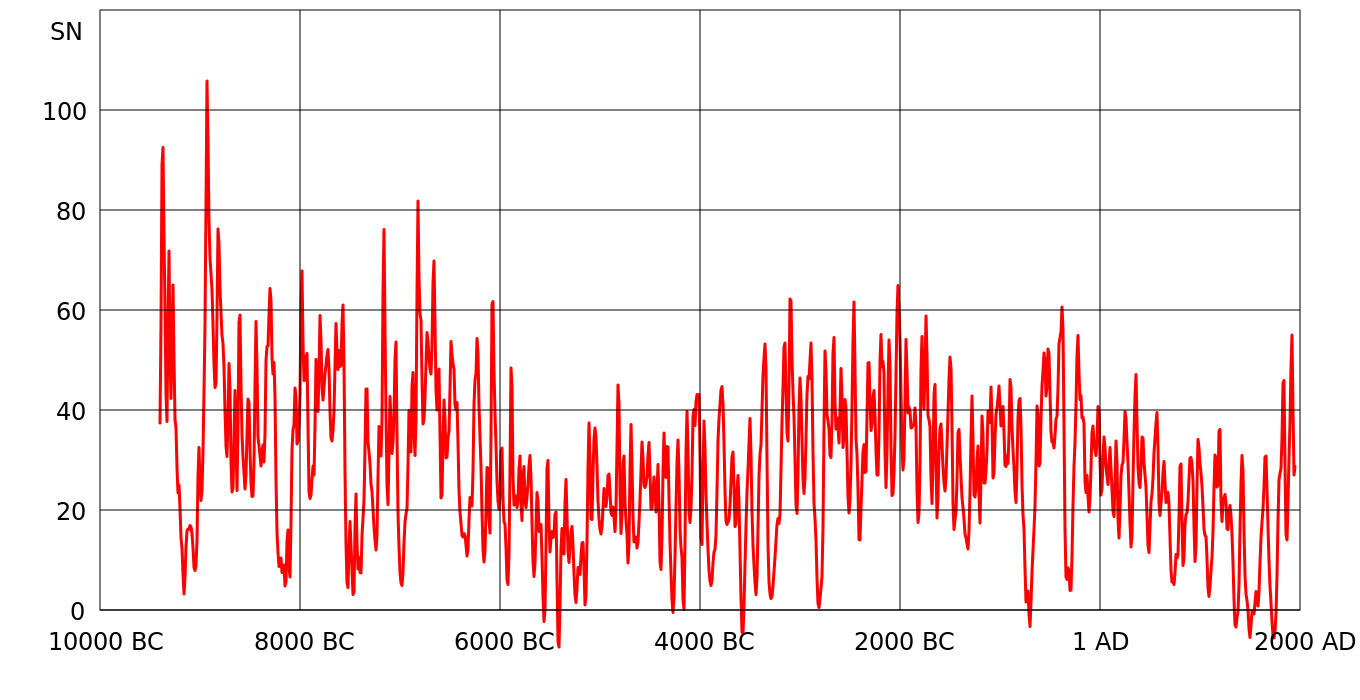
\includegraphics[height=7cm]{Predavanja/05_SatLastPolozaj/figs/Sunspots_11000_years.png}
	\caption{Od 1750 naprej štejemo število peg na Soncu, dotlej je število ocenjeno posredno iz \textit{geoloških koledarjev}.}
	\label{fig:Gnss_Polozaj:11tisocLetSN}
\end{figure}



\paragraph{Paragraph Heading} %
Your text goes here.

\subparagraph{Subparagraph Heading.} Your text goes here.%
%
\index{paragraph}
% Use the \index{} command to code your index words
%
% For tables use
%
\begin{table}
\centering
\caption{Please write your table caption here}
\label{tab:1}       % Give a unique label
%
% For LaTeX tables use
%
\begin{tabular}{lll}
\hline\noalign{\smallskip}
first & second & third  \\
\noalign{\smallskip}\hline\noalign{\smallskip}
number & number & number \\
number & number & number \\
\noalign{\smallskip}\hline
\end{tabular}
\end{table}
%
%
% For figures use
%
%ship-img-master768.jpg

\begin{figure}
	\centering
	\includegraphics[height=3.6cm]{Predavanja/05_SatLastPolozaj/figs/170616UssFitzgeraldShipCollision.jpg}
	\hspace*{0.5cm}
	\includegraphics[height=3.6cm]{Predavanja/05_SatLastPolozaj/figs/170713NNT265025.jpg}%ShipImgMaster768.jpg}
	\caption{ \textbf{Škodi}, nastali ob trčenju 17. junija 2017 ob polotoku Izu, jugozahodno od Tokia (levo) na Filipinih registrirani kontejnerski ladji ACX Crystal, (Japan’s 3rd Regional Coast Guard Headquarters/AP). (desno) pod vodno linijo na vojaški ladji USS Fitzgerald (Christian Senyk, U.S. Navy).} %na vojaški ladji USS Fitzgerald (Kazuhiro Nogi/AFP — Getty Images
	\label{fig:Gnss_Polozaj:poslediceTrcenja}       % Give a unique label
\end{figure} 




% If not, use
%\picplace{5cm}{2cm} % Give the correct figure height and width in cm
%
% For built-in environments use
%
\begin{theorem}
Theorem text goes here.
\end{theorem}
%
% or
%
\begin{lemma}
Lemma text goes here.
\end{lemma}
%
%
\section{Kaj gre lahko narobe?}
Analize osvetljujejo verjetne vzroke za ladijske nesreče. Opremljenost ladij z elektronskimi napravami spremljajo usposabljanja posadk za učinkovito in varno delo z novimi napravami. Poenostavljanja naučenih pravil in nepremišljena uporaba avtomatiziranih sistemov večajo verjetnost za neželene dogodke. Svoj delež prispevajo tudi manj običajni naravni pogoji in v današnjem svetu tudi želje po uničenju plovila s pomočjo kibernetskega napada. (\ref{fig:Gnss_Polozaj:poslediceTrcenja})    
%http://cimsec.org/ships-crashing-competence-overload-cyber-considerations/33865

% Problems or Exercises should be sorted chapterwise
\section*{Problems}
\addcontentsline{toc}{section}{Problems}
%
% Use the following environment.
% Don't forget to label each problem;
% the label is needed for the solutions' environment
\begin{prob}
\label{prob1}
The problem\footnote{Footnote} is described here. The
problem is described here. The problem is described here.
\end{prob}

\begin{prob}
\label{prob2}
\textbf{Problem Heading}\\
(a) The first part of the problem is described here.\\
(b) The second part of the problem is described here.
\end{prob}



%

%
\chapter{Sistemi za določanje tujega položaja}
\label{Ch_Radar} % Always give a unique label
% use \chaptermark{}
% to alter or adjust the chapter heading in the running head

Z napravami za določanje tujega položaja smo sposobni določiti relativni ali absolutni položaj tujega objekta. V relativnem načinu je izhodišče prostora točka iz katere opazujemo okolico, v absolutnem načinu je izhodišče masno središče Zemlje.

\begin{figure}
	\centering
	\includegraphics[height=4.5cm]{Predavanja/06_DolocTujegaPolozaja/figs/RadarjevoObzorjeInDoseg.png}
	\caption{Radarsko obzorje je določeno s pogoji atmosfere, doseg radarja pa z lastnostmi snopa in antene ter z lastnostmi objektov.}
	\label{fig:RadarObzorjeDoseg}       % Give a unique label
\end{figure} 
%


%DOC http://www.furuno.com/en/products/radar
radar, SAR
določanje razdalje do objekta
%http://www.radartutorial.eu/01.basics/Distance-determination.en.html
določanje azimuta objekta
%http://www.radartutorial.eu/01.basics/Direction-determination.en.html
največja enoumno določljiva razdalja
%http://www.radartutorial.eu/01.basics/Maximum%20Unambiguous%20Range.en.html
razdalja do najbližje zaznavnega objekta
%http://www.radartutorial.eu/01.basics/Minimal%20Measuring%20Range.en.html
razločljivost po razdalji
%http://www.radartutorial.eu/01.basics/Range%20Resolution.en.html
točnost določanja tujega položaja
%http://www.radartutorial.eu/01.basics/Radars%20Accuracy.en.html

NOAA radar
%http://player.slideplayer.com/16/5227228/#

Ali fizična velikost odsevnika vpliva na možnost zaznavanja plovil.
Če ima ladja večjo efektivno odsevno površino (v ta parameter pade fizična velikost, material, oblika, relativna usmerjenost glede na os radarske antene), je možnost zaznavanja ladje večja.


\section{Section Heading}
\label{sec:1}
% Always give a unique label
% and use \ref{<label>} for cross-references
% and \cite{<label>} for bibliographic references
% use \sectionmark{}
% to alter or adjust the section heading in the running head
Your text goes here. Use the \LaTeX\ automatism for your citations
\cite{monograph}.

\subsection{Subsection Heading}
\label{sec:2}
Your text goes here.

\begin{equation}
\vec{a}\times\vec{b}=\vec{c}
\end{equation}

\subsubsection{Subsubsection Heading}
Your text goes here. Use the \LaTeX\ automatism for cross-references as
well as for your citations, see Sect.~\ref{sec:1}.

\paragraph{Paragraph Heading} %
Your text goes here.

\subparagraph{Subparagraph Heading.} Your text goes here.%
%
\index{paragraph}
% Use the \index{} command to code your index words
%
% For tables use
%
\begin{table}
\centering
\caption{Please write your table caption here}
\label{tab:1}       % Give a unique label
%
% For LaTeX tables use
%
\begin{tabular}{lll}
\hline\noalign{\smallskip}
first & second & third  \\
\noalign{\smallskip}\hline\noalign{\smallskip}
number & number & number \\
number & number & number \\
\noalign{\smallskip}\hline
\end{tabular}
\end{table}
%
%
% For figures use
%
\begin{figure}
\centering
% Use the relevant command for your figure-insertion program
% to insert the figure file.
% For example, with the option graphics use
\includegraphics[height=4cm]{figure}
%
% If not, use
%\picplace{5cm}{2cm} % Give the correct figure height and width in cm
%
\caption{Please write your figure caption here}
\label{fig:1}       % Give a unique label
\end{figure}
%
% For built-in environments use
%
\begin{theorem}
Theorem text goes here.
\end{theorem}
%
% or
%
\begin{lemma}
Lemma text goes here.
\end{lemma}
%
%
% Problems or Exercises should be sorted chapterwise
\section*{Vprašanja v razmislek in poglobitev}
\addcontentsline{toc}{section}{Problems}
%
% Use the following environment.
% Don't forget to label each problem;
% the label is needed for the solutions' environment
\begin{prob}
\label{prob1.ZaznavanjeRadarja}
\textbf{Omejitve zaznavanja z radarjem}\\
(a) Koliko mikrosekund bo radarski signal potreboval do 6NM oddaljenega objekta in nazaj?\\
(b) Na koliko navtičnih milj bi lahko ladijski radar enoumno zaznaval objekte, če ima nastavljeno frekvenco ponavljanja impulzov ($f_{PR}$) na 3000 Hz? Koliko mora nastaviti  $f_{PR}$, da bo enoumno določal oddaljenosti objektov do 24NM? \\
(c) Plovilo je opremljeno z radarjem z dosegom 32 NM.  Radarska antena je na plovilu nameščena na višini 35,0 metrov nad gladino morja. Plovilo se približuje skalnati obali s stenami visokimi 7,0 m. Pojasnite na katerih oddaljenostih od obale je možno pričakovati, da se bo skalnata obala pojavila na radarskemu zaslonu? \\
(č) Od česa je odvisna najmanjša razdalja odkrivanja? Od česa je odvisen najmanjši doseg radarja? Izračunaj najmanjši doseg, če sega $H_{antene}$ = 25m nad gladino, širina snopa v vertikalni ravnini $23^{\circ}$.\\
(d) Koliko znaša najmanjša zaznavna razdalja radarja, če je čas vzpostavitve TR stikala 1,5 mikrosekunde, čas trajanja impulzov pa 0,5 mikrosekunde?
\end{prob}

\begin{prob}
\label{prob2.Odkrivanje}
\textbf{Meje odkrivanja}\\
(a) \\
(b) The second part of the problem is described here.
\end{prob}



%

\include{Predavanja/07_PodOmrNMEA2000/chP_PodOmrNMEA2000}
%
\chapter{Povzetek sodobnih elektronskih navigacijskih pripomočkov}
\label{intro} % Always give a unique label
% use \chaptermark{}
% to alter or adjust the chapter heading in the running head

ECDIS, združitev zajemov večih senzorjev in zagotavljanje varne plovbe

%RADAR overlay vs. ECDIS: https://www.linkedin.com/groups/2247966/2247966-6191161999863345153
%=======================
%a radar overlay feature never replaces a full radar. 
%While the radar is a pure collision avoidance tool, radar overlay is meant to enhance the capabilities of the ECDIS. 
%Unfortunately, there is little control in the industry as to what radar overlay should look like. You can find anything from preprocessed radar pictures (as mentioned by Jaap) to fully tune-able radar inputs for the ECDIS. 
%Without knowing the vessel specifics, a safe rule of thumb is: radars have to be redundant, ECDIS have to be redundant, any equipment needs to carry a wheelmark (for marine use) and has to be type approved (fit for purpose) when fulfilling a primary navigational function; there are many exceptions and additions to the these ground rules, depending on: vessel size, vessel type, class, flag, trade area, etc
%In addition, you should find out what category of vessel we are talking. Is the ECDIS primary mean of navigation where you have choise of two independent workstation (paperless) or one ECDIS and full supplement of charts for intended voyage. Remember EDIS require only input of position (GPS/DGPS) heading device and log. Doesn't need to be connected with AIS nor radar or any other device. Radar overlay is only a funcionality of ECDIS when radar input is connected. Just like chart radar when you have MFDs or input from NAVTEX on ECDIS or ... Depends what you want, just cover requirements or make integrated bridge system. Legal requirements is must, other is question of space and budget.
%Radar Overlay is used for determining the position by alternate source to meet best navigation practices of "2 means of position fixing" method. Radar overlay as it describes is an overlay and should be briefly referred by navigator to verify the GPS positions. Most often the visual quality of data on the ENC gets degraded / cluttered when radar overlay is used. ECDIS is a chart (ENC-Electronic chart) and is not used for collision avoidance purpose, as described by Seven also. Both have separate functions. I am not aware of regulatory requirements, Fundamentally ENC is still a chart and radar is one of navigation aid to assist the navigating officer for safe navigation, except it can now be viewed on one screen. Only thing i want to say is too much information on one screen is confusing for the navigator. Hence it is better to keep navaids as independent as possible.
%=======
%Hi and thanks for your comments and assistant in my question. I now have a good picture and well based knowledge to assist my customer. The key is that as many of you has underlined radar is a tool for collision avoidance and that has to be the prime mission. The option with radar overlay is a enhance to the Ecdis picture in helping the navigator.

%http://www.consilium.se/news/consilium-receives-first-order-its-new-web-based-remote-playback-service
%VDR Consilium receives the first order for its new web-based Remote Playback service

\section{Section Heading}
\label{sec:1}
% Always give a unique label
% and use \ref{<label>} for cross-references
% and \cite{<label>} for bibliographic references
% use \sectionmark{}
% to alter or adjust the section heading in the running head
Your text goes here. Use the \LaTeX\ automatism for your citations
\cite{monograph}.

\subsection{Subsection Heading}
\label{sec:2}
Your text goes here.

\begin{equation}
\vec{a}\times\vec{b}=\vec{c}
\end{equation}

\subsubsection{Subsubsection Heading}
Your text goes here. Use the \LaTeX\ automatism for cross-references as
well as for your citations, see Sect.~\ref{sec:1}.

\paragraph{Paragraph Heading} %
Your text goes here.

\subparagraph{Subparagraph Heading.} Your text goes here.%
%
\index{paragraph}
% Use the \index{} command to code your index words
%
% For tables use
%
\begin{table}
\centering
\caption{Please write your table caption here}
\label{tab:1}       % Give a unique label
%
% For LaTeX tables use
%
\begin{tabular}{lll}
\hline\noalign{\smallskip}
first & second & third  \\
\noalign{\smallskip}\hline\noalign{\smallskip}
number & number & number \\
number & number & number \\
\noalign{\smallskip}\hline
\end{tabular}
\end{table}
%
%
% For figures use
%
\begin{figure}
\centering
% Use the relevant command for your figure-insertion program
% to insert the figure file.
% For example, with the option graphics use
\includegraphics[height=4cm]{figure}
%
% If not, use
%\picplace{5cm}{2cm} % Give the correct figure height and width in cm
%
\caption{Please write your figure caption here}
\label{fig:1}       % Give a unique label
\end{figure}
%
% For built-in environments use
%
\begin{theorem}
Theorem text goes here.
\end{theorem}
%
% or
%
\begin{lemma}
Lemma text goes here.
\end{lemma}
%
%
% Problems or Exercises should be sorted chapterwise
\section*{Problems}
\addcontentsline{toc}{section}{Problems}
%
% Use the following environment.
% Don't forget to label each problem;
% the label is needed for the solutions' environment
\begin{prob}
\label{prob1}
The problem\footnote{Footnote} is described here. The
problem is described here. The problem is described here.
\end{prob}

\begin{prob}
\label{prob2}
\textbf{Problem Heading}\\
(a) The first part of the problem is described here.\\
(b) The second part of the problem is described here.
\end{prob}



%

\include{Predavanja/09_PovzNapakInOdpravlj/chP_PovzNapakInOdpravlj}
%
\chapter{Splošen pregled komunikacijskih ladijskih naprav in osnove GMDSS}
\label{intro} % Always give a unique label
% use \chaptermark{}
% to alter or adjust the chapter heading in the running head

%tukaj je JRCjeva aplikacija za spremljanje prisotnih wi-fi omrežij, hitrosti prenosov...
% Lahko nastavita kako pogosto bosta oddajali opažanja.
% https://play.google.com/store/apps/details?id=ec.europa.eu.smartmonitor
%tukaj pa AKOSova za fiksna omrežja
% http://www.komuniciraj.eu/test-hitrosti#

% https://www.navcen.uscg.gov/?pageName=GMDSS
%In 1979, a group of experts drafted the International Convention on Maritime Search and Rescue, which called for the development of a global search and rescue plan.  This group also passed a resolution calling for the development of a Global Maritime Distress and Safety System (GMDSS) to provide the communication support needed to implement the global search and rescue plan.  

%This system, which the world's maritime nations - including the United States - have implemented, is based upon a combination of satellite and terrestrial radio services and has changed international distress communications from being primarily ship-to-ship-based to primarily ship-to-shore-based (Rescue Coordination Center).  

%For more information, visit the International Maritime Organization (IMO) Global Maritime and Distress Safety Systems Overview and/or download a GMDSS Inspection Checklist. http://transition.fcc.gov/eb/ShipInsp/gmdss_checklist.pdf

%GMDSS: the next generation, As IMO’s review of the GMDSS continues, Iridium is pushing for a place at the table while Inmarsat is looking to evolve its offering to include ‘safety as a service’, Digital Ship October 2015 page 12

%Fairway Issue No. 30 Spring, 2010
%In introducing this meeting on board HQS Wellington Kim Fisher said that he had originally suggested the title as a joke since everything nowadays was e something, eNavigation, eCommerce, but that the joke had returned to haunt him as eGMDSS could become a reality. GMDSS is only ten years old, but the idea goes back much further. Under SOLAS 1960 passenger ships and cargo vessels over 1,600 gt. had to carry radio telegraph and monitor 500 kHz, while smaller vessels carried radio telephone, keeping watch on 2,182 kHz. SOLAS 1974 had introduced VHF radio telephony, keeping watch on channel 16. Watchkeeping was manual, assisted by radio telegraph and radio telephone auto alarms. The range of about 150 nm. under normal conditions was of limited use for ocean passages.
%GMDSS introduced the idea of distress alerts, notified, not directly to ships, but to a shoreside Rescue Co-ordination Centre by terrestrial or satellite communications. The
%RCC would then alert ships in the area and coordinate rescue attempts. This involved dividing the world into Maritime Search and Rescue regions. It was intended to consign morse code, UHF transmissions, 121.5 MHz and manual watchkeeping to history, bringing in their place satellite EPIRBs, SART, NAVTEX, Inmarsat, SafetyNET, DSC and NBDP. Two other changes were brought in at the same time – distress could be applied to persons as well as ships, and the calling party selected the channel for subsequent communications.

%Chris Blockley-Webb from the Navigation Safety Branch of the MCA presented a review of, and modernization of, GMDSS, stating that it was a partnership between
%many administrative bodies, and that it would take twenty years to achieve full implementation. He quoted nine distinct functions of GMDSS.
%Ship to shore distress alerts by two separate and independent means. Shore to ship distress alerts. Ship to ship distress alerts. Search and rescue co-ordination communications.
%On scene communications. Locating signals Maritime safety information. General radio communications. Bridge to bridge communications. These were gone into in some detail. Moving on to the current situation Chris Blockley-Webb described COMSAR 14/7/1 and associated papers, subscribed to by the UK, USA, Chile, France and Australia. With the plans for eNavigation, GMDSS must be part of this, but there is currently no indication of which direction it will take nor how they will be linked. There are likely to be scoping exercises at the next two COMSAR sessions, with review and modernization of the system taking place in 10, 15 and 20 years time. Bob Ball, Electrical Superintendent of BP Shipping, had been booked as the next
%contributor but had been unable to attend at short notice. Instead, Kim Fisher showed a few slides that had been provided. In the first of these it was pointed out that HF radio
%was not well understood by deck officers, that it was more complicated to operate than Sat-C, while having the same costs, but needing greater maintenance. Sat-C, on the other
%hand, was already carried in all sea area A3 vessels for the receipt of SafetyNET, and was carried by most other vessels for LRIT purposes. BP Shipping advocates the dual
%Sat-C approach, with MF / HF fitted purely to meet legislation. They suggest that VHF is still a good solution for sea area A1, being relatively inexpensive and simple to use,
%and that sea areas A2 and A3 be combined and Sat-C carriage be mandatory for this new sea area.
%
%Peter Blackhurst, Head of Maritime Safety Services at Inmarsat, pointed out that technology was changing faster than the regulations and asked if we wanted a slimline, easy operating system that provided the necessary service or an all singing, all dancing system that was swamped with communications protocols. We already had IP Connectivity, SMS and cross-network connectivity, but were being restricted in the use of the radio spectrum. The system could be clogged by communications protocols during distress working, so it was time to look at it again.
%With Inmarsat’s latest I-4 satellites, offering Broadband Global Area Network (BGAN), we now had one device connecting to three networks. Messages could be streamed between the users terminal, voice and ISDN phone or a computer, via the satellite, to an Internet Provider’s router. From there it could go by a Streaming IP network using a guaranteed Quality of Service line or a Standard IP Network by either the internet or a local area network. It could also use a Circuit Switched Network to deliver voice messages to a phone. These systems, and their differences, were described. Safety services supported by Inmarsat were also described, together with possible future developments for both voice and data transmission. Other technologies include the digitization of data for transmission by VHF and the use of WiMax, but all future changes needed to avoid making the earlier analogue systems obsolete. Future eNavigation may eventually use the same communications system as GMDSS.
%The final speaker was Dr. Martin Ziarati , Director of C4FF and a partner in MarEdu Partnership. He pointed out that, as equipment changes and possibly becomes more complex, there is a greater need for training. Citing STWC, which was introduced 15 years ago, research has shown deficiencies, and best practices need to be used worldwide. With the loss of morse code, all mariners are expected to communicate in English, yet that is not the native language of the majority of seafarers. New automatic systems need understanding and emergency situations put people under pressure. Training is required, but how to provide it?
%C4FF is a training and distance learning project that operates through the internet via its web sites. It is supported by several organizations such as BTEC, MNTB, MCA, EDEXCEL and NVQ/SVQ. Where relevant, on-line simulators are used, with over 23,000 users in 190 countries. The simulators are not generic, but are specific to each manufacturer’s equipment. Training is available in ten languages and, being funded by the EU, is free to the user. The web sites through which this is delivered are:
%www.c4ff.co.uk www.egmdss.com www.martel.pro www.maritime-test.org www.maredu.co.uk www.eWoggle.co.uk 

%Following the presentations there were some questions:
%Q: Ships used to carry a Radio Officer, who could not only use the equipment but also repair it when it failed. Who fixes this kit when it is faulty?
%A: There will be a requirement to carry duplicate equipment so that one will carry on working should one become inoperative.
%Q: DSC has proved unreliable. When will it be dumped?
%A: For a time I worked in an MRCC. During that time there were three cases of a person being rescued and families reunited using DSC. The situation is open to discussion.
%Q: Satellite communications are liable to fail. How can this be prevented?
%A: If it happens, GPS satellites are likely to fail as well and the world would be in a mess. It is said that there is a need for alternatives to satellite communication. WiMax is being used successfully in Singapore and digitized VHF experiments for AIS messaging are being carried out in Norway.


Your text goes here. Separate text sections with the standard \LaTeX\
sectioning commands.

\section{Section Heading}
\label{sec:1}
% Always give a unique label
% and use \ref{<label>} for cross-references
% and \cite{<label>} for bibliographic references
% use \sectionmark{}
% to alter or adjust the section heading in the running head
Your text goes here. Use the \LaTeX\ automatism for your citations
\cite{monograph}.

\subsection{Subsection Heading}
\label{sec:2}
Your text goes here.

\begin{equation}
\vec{a}\times\vec{b}=\vec{c}
\end{equation}

\subsubsection{Subsubsection Heading}
Your text goes here. Use the \LaTeX\ automatism for cross-references as
well as for your citations, see Sect.~\ref{sec:1}.

\paragraph{Paragraph Heading} %
Your text goes here.

\subparagraph{Subparagraph Heading.} Your text goes here.%
%
\index{paragraph}
% Use the \index{} command to code your index words
%
% For tables use
%
\begin{table}
\centering
\caption{Please write your table caption here}
\label{tab:1}       % Give a unique label
%
% For LaTeX tables use
%
\begin{tabular}{lll}
\hline\noalign{\smallskip}
first & second & third  \\
\noalign{\smallskip}\hline\noalign{\smallskip}
number & number & number \\
number & number & number \\
\noalign{\smallskip}\hline
\end{tabular}
\end{table}
%
%
% For figures use
%
\begin{figure}
\centering
% Use the relevant command for your figure-insertion program
% to insert the figure file.
% For example, with the option graphics use
\includegraphics[height=4cm]{figure}
%
% If not, use
%\picplace{5cm}{2cm} % Give the correct figure height and width in cm
%
\caption{Please write your figure caption here}
\label{fig:1}       % Give a unique label
\end{figure}
%
% For built-in environments use
%
\begin{theorem}
Theorem text goes here.
\end{theorem}
%
% or
%
\begin{lemma}
Lemma text goes here.
\end{lemma}
%
%
% Problems or Exercises should be sorted chapterwise
\section*{Problems}
\addcontentsline{toc}{section}{Problems}
%
% Use the following environment.
% Don't forget to label each problem;
% the label is needed for the solutions' environment
\begin{prob}
\label{prob1}
The problem\footnote{Footnote} is described here. The
problem is described here. The problem is described here.
\end{prob}

\begin{prob}
\label{prob2}
\textbf{Problem Heading}\\
(a) The first part of the problem is described here.\\
(b) The second part of the problem is described here.
\end{prob}



%

%
\chapter{Sistem za krmarjenje ladje }
\label{intro} % Always give a unique label
% use \chaptermark{}
% to alter or adjust the chapter heading in the running head

Krmiljenje in regulacija plovbe na sodobni ladji

\begin{figure}
	\centering
	\includegraphics[height=4cm]{Predavanja/11_SodobnoKrmarjenjeLadje/figs/SLK4p1.png}
	\caption{Magnetni kompas z induktivnim izhodom, ki daje položaj igle.}%Gpsmap60CS, Garmin}
	\label{fig:MagnetniKompasInduktIzhod}       % Give a unique label
\end{figure}

\begin{figure}
	\centering
	\includegraphics[height=6cm]{Predavanja/11_SodobnoKrmarjenjeLadje/figs/SLK4p2.png}
	\caption{Vrtavčni kompas z induktivnim izhodom.}%Gpsmap60CS, Garmin}
	\label{fig:VrtavcniKompasInduktIzhod}       % Give a unique label
\end{figure}

The term \textbf{starboard, (StB)} derives from the Old English steorbord, meaning the side on which the ship is steered. Before ships had rudders on their centrelines, they were steered with a steering oar at the stern of the ship and, because more people are right-handed, on the right-hand side of it. Port and starboard are nautical terms for left and right, respectively. \textit{Port, (BB) is the left-hand side of or direction from a vessel, facing forward}. \textit{Starboard is the right-hand side, facing forward}. Since port and starboard never change, they are unambiguous references that are not relative to the observer. In Old English the word was bcbord, of which cognates are used in other European languages, for example as the German backbord (BB). (wiki)

\begin{figure}
	\centering
	\includegraphics[width=\textwidth]{Predavanja/11_SodobnoKrmarjenjeLadje/figs/SLK4p16.png}
	\caption{Želena vrednost (handsteuerung) se z odštevanjem v od trenutne smeri, ki jo kaže kompas, spreminja v krmilne signale za dvigovanje tlaka ali v valju 'starboard' StB ali v valju 'backbord', ki z ustrezno silo pritiskata na ploščo krmila (BB).}%Gpsmap60CS, Garmin}
	\label{fig:SamodejnoKrmarjenjeStB_BB}       % Give a unique label
\end{figure}






\section{Section Heading}
\label{sec:1}
% Always give a unique label
% and use \ref{<label>} for cross-references
% and \cite{<label>} for bibliographic references
% use \sectionmark{}
% to alter or adjust the section heading in the running head
Your text goes here. Use the \LaTeX\ automatism for your citations
\cite{monograph}.

\subsection{Subsection Heading}
\label{sec:2}
Your text goes here.

\begin{equation}
\vec{a}\times\vec{b}=\vec{c}
\end{equation}

\subsubsection{Subsubsection Heading}
Your text goes here. Use the \LaTeX\ automatism for cross-references as
well as for your citations, see Sect.~\ref{sec:1}.

\paragraph{Paragraph Heading} %
Your text goes here.

\subparagraph{Subparagraph Heading.} Your text goes here.%
%
\index{paragraph}
% Use the \index{} command to code your index words
%
% For tables use
%
\begin{table}
\centering
\caption{Please write your table caption here}
\label{tab:1}       % Give a unique label
%
% For LaTeX tables use
%
\begin{tabular}{lll}
\hline\noalign{\smallskip}
first & second & third  \\
\noalign{\smallskip}\hline\noalign{\smallskip}
number & number & number \\
number & number & number \\
\noalign{\smallskip}\hline
\end{tabular}
\end{table}
%
%
% For figures use
%
\begin{figure}
\centering
% Use the relevant command for your figure-insertion program
% to insert the figure file.
% For example, with the option graphics use
\includegraphics[height=4cm]{figure}
%
% If not, use
%\picplace{5cm}{2cm} % Give the correct figure height and width in cm
%
\caption{Please write your figure caption here}
\label{fig:1}       % Give a unique label
\end{figure}
%
% For built-in environments use
%
\begin{theorem}
Theorem text goes here.
\end{theorem}
%
% or
%
\begin{lemma}
Lemma text goes here.
\end{lemma}
%
%
% Problems or Exercises should be sorted chapterwise
\section*{Problems}
\addcontentsline{toc}{section}{Problems}
%
% Use the following environment.
% Don't forget to label each problem;
% the label is needed for the solutions' environment
\begin{prob}
\label{prob1}
The problem\footnote{Footnote} is described here. The
problem is described here. The problem is described here.
\end{prob}

\begin{prob}
\label{prob2}
\textbf{Problem Heading}\\
(a) The first part of the problem is described here.\\
(b) The second part of the problem is described here.
\end{prob}



%

%\appendix
%\include{appendix}
\include{part_vaje}
%
\chapter{Splošna navodila za izdelavo seminarske naloge }
\label{ch:NavodSeminar}

\textit{Kaj morate vedeti pred začetkom dela?} Najprej si preberite splošna navodila v tem poglavju. Ko boste vključeni v eno od skupin pa si boste skupaj izbrali eno izmed nalog. Študijske naloge boste opravljali v različnih prostorih: v predavalnici, v navtičnem, v komunikacijskem simulatorju, v laboratoriju za elektrotehniko in na plovilih, ki bodo poleg nujnega vložka predavateljev tudi z vašim prispevkom prirejena za zastavljene naloge.

\textbf{Lastne izkušnje} si boste s seminarskimi nalogami oplemenitili, če jih boste delali premišljeno in boste svoj lastni napredek v dojemanju delili tudi z drugimi v skupini in v letniku. Ne bojte se pravočasno vprašati predavatelje. Oprite se na sistem enomesečnega dela (podrobneje v poglavju \ref{sec:OpisDela}, pomoč\footnote{\textbf{pomoč} razlaga simbolov: o .. samostojno delo v skupini, x .. računajte na pomoč predavateljev}), v katerega kar pogumno vstopite in vztrajajte.
 
\begin{table}[!htbp] 
	\caption{Faze enomesečnega dela s seminarsko nalogo: časovni roki in pričakovani rezultati.}
	\vspace{2mm}
	\begin{center}
		{\small
			\begin{tabular}{l||c|c|l|c}\hline
			faza dela	   & rok za dokončanje & pomoč & rezultati 			     & opombe \\ \hline \hline
			(1) skupine    & 1 teden           & x     & seznam članov           & vprašanja po e-pošti\\ \hline
			(2) moja naloga& 1 teden           & o     & naloge članov sporočim & srečanje skupine\\ \hline
			(3) lab. okolje&                   & (x)   & zapisi, logi, slike     & najava, odložišče \\ \hline
			(4) analiza	   & 1 teden           & x     & analize in načrti    	 & čimbolj samostojno\\ \hline
			(5) del. okolje&                   & x     & zapisi, logi, slike     & vreme, plovila  \\ \hline
			(6) navodila   & 1 teden           & (x)   & navodila                &\textit{za telebane}\\ \hline
			(7) pisanje	   &                   & o     & poročilo                & po \TeX predlogi \\ \hline
			(8) vaših 5 minut& spremljaj objave& o     & predstavitev            & flomaster, tabla \\ \hline
			\textbf{po predstavitvi}&          &       & ocena seminarja         & vklj. medsebojne ocene\\ \hline
				            &                  &       & zbornik poročil         &      \\ \hline
			\end{tabular}
		}
	\end{center}
	\label{tab:faze_dela}
\end{table}

V skoraj vseh fazah dela vam bomo torej na voljo predavatelji in strokovni sodelavci, da boste nalogo dokončali v predvidenem roku.

\section{Enomesečno delo}
\label{sec:OpisDela}

Na prvem predavanju vam bomo predavatelji predstavili načrt dela. Po osnovanju skupin se boste seznanili s potrebno opremo in si razdelili predvidene naloge. Poskuse boste opravljali v predvidenih varnih okoljih laboratorija ali simulatorja, dobljene rezultate boste analizirali po skupinah. Nato boste izvedli poskuse v delovnih okoljih, \textit{ko bo vremenska napoved ugodna, ne odlašajte}. Ko boste poskuse opravili, boste takoj po njih napisali navodila za izvedbo poskusov in sestavili poročila po predlogi (glej poglavje \ref{ch:Poroc_Vzorec} in uporabi predlogo \ref{ch:seminar_report_template}). Delo boste sklenili s petminutno predstavitvijo skupnega dela.     

\textbf{Oceno} seminarske naloge oz. ali jo boste opravili, boste sooblikovali sami. Poleg kakovosti izvedbe, poročila in predstavitve bo ocena vključevala tudi, če ste se držali rokov. 

Če bo katera od nalog od posameznih članov zahtevala bistveno več časa kot 15 ur, boste ob predložitvi dokumentacije in pogovoru s predavatelji lahko oproščeni katere od laboratorijskih vaj. Vsaka skupina pošlje na \textit{kratko usposabljanje} (do pol ure ) enega člana, ki bo odgovoren za obdelavo oz. prikaz rezultatov z grafom. V večini skupin boste vrisovali točke, kurze na svoje pomorske karte.


% Problems or Exercises should be sorted chapterwise
\section*{Naloge}
\addcontentsline{toc}{section}{Naloge}
Če vas zanima ..
\begin{prob}
	\label{Nal:SplNavCas}
	 \textit{Kakšen pomen ima čas v pomorstvu?}, si podrobnosti za izdelavo preberite v poglavju \ref{Vaje:Cas}.
\end{prob}

\begin{prob}
	\label{Nal:SplNavMem}
	\textit{Kaj lahko poveste o poteku plovbe, če dobite v roke časovni graf ali pospeškov ali kotne hitrosti obračanje okoli osi plovila ali zabeleženih magnetnih polj?}, si podrobnosti za izdelavo preberite v poglavju \ref{Vaje:RekonsMems}.
\end{prob}


\begin{prob}
	\label{Nal:SplNavKart}
	\textit{Kako najdete koordinato na morju, izmerite slanost, motnost in globino?}, si podrobnosti za izdelavo preberite v poglavju \ref{Vaj:KartSlanGlob}.
\end{prob}

\begin{prob}
	\label{Nal:SplNavKomp}
	\textit{Kaj morate vedeti o konkretnem kompasu, kako ga pripravite za plovbo in kako plovbo z njim tudi izvedete?}, si podrobnosti za izdelavo preberite v poglavju \ref{Vaje:VrtKompas}.
\end{prob}

\begin{prob}
	\label{Nal:SplNavVes}
	\textit{Kako vesoljsko vreme vpliva na komunikacijo in navigacijo na Zemlji?}, si podrobnosti za izdelavo preberite v poglavju \ref{Vaje:VesVrem}.  
\end{prob}

\begin{prob}
	\label{Nal:SplNavGns}
	\textit{Katere omejitve uporabe podatkov iz sprejemnikov GNSS srečamo v pomorski praksi?}, si podrobnosti za izdelavo preberite v poglavju \ref{Vaje:GnssPraks}.
\end{prob}







%

%
\chapter{Čas v podatkih na morju}
\label{sec:v_cas} 

Zgodovinsko, je bil čas v navigaciji eden od glavnih elementov določanja položaja. Čas so uporabljali za določanje zemljepisne dolžine ($\lambda$ ali ang. \emph{Longitude}). Pred izumom ure ali  kronometra (grško \emph{kronos} pomeni čas) je bila navigacija na morju zelo otežena. Le s pomočjo izmere razdalje so lahko napovedovali zemljepisno dolžino. Vsak si lahko predstavlja kakšno napako so pri tem storili. Prevoženo razdaljo so računali iz povprečne hitrosti, ki pa je bila obremenjena s hudo napako.

\begin{figure}[!h]
	\centering \includegraphics[width=8cm]{Vaje/CasPomorstvo/figs/kronometer_01.png}
	\caption{Navtični kronometer.}
\end{figure}

\section{Opis vaje}
\label{sec:v_cas_opis}
Namen vaje je seznanitev študenta z razumevanjem časa. Čas ima več oblik in natančnosti. Čas lahko merimo skozi ponavljajoče se astronomske dogodke (dan/noč, mesečeve mene, zenit sonca, $\ldots$), čakanje punce na želežniškem peronu, z atomsko uro in podobno. Skratka pojem časa je zelo relativen, zato je potrebno definirati kateri čas bomo uporabljali v tej nalogi.

\subsection{Dogovor o zapisu in uporabi časa:}
\begin{itemize}
	\item \textsc{Format zapisa}:\\[2mm]
	Čas bomo zapisovali v obliki\\[2mm] 
	\textbf{HH:MM:SS.ss},\\[2mm]
	kjer je \textbf{H}-ura, \textbf{M}-minuta, \textbf{S}-sekunda in \textbf{s}-delež sekunde v decimalni obliki. Natančnost časovne meritve bomo vedno zapisali na dve decimalki natančno. Kot primer zapišimo:\\[2mm] 
	%
	13:12:10.33 - 13h, 12min, 10.33sek; urni zapis je v 24h\\
	%
	\item \textsc{Časovna zona}:\\[2mm]
	Enako je potrebno definirati v kateri časovni zoni bomo čas zapisovali. Vedno je potrebno čas zapisati v UTC. Za podrobnosti, kaj UTC pomeni si poglejte na splet\\[2mm] \url{https://en.wikipedia.org/wiki/Coordinated_Universal_Time}\\
	
	\item \textsc{Časovna referenca}:\\[2mm]
	Za časovno referenco vzemite enega od časovnih strežnikov, kot na primer:\\[2mm]
	\url{http://www.ijs.si/time/ijs-time.html}\\[2mm]
	Tako boste imeli svoje elektronske naprave dobro sinhronizirane.\\
\end{itemize}

Kot smo videli imamo v dogovoru definirano uporabo časovne reference. Čas venomer prislonimo na določeno časovno referenčno točko. Danes večino meritev v pomorstvu sinhroniziramo prav s časom, ki ga dobimo iz GPS sprejemnika. Sateliti, ki jih uporabljamo za določanje položaja imajo izjemno natančen čas, ki ga lahko spremljamo na GPS sprejemniku.



\subsection{Izvedba vaje}
Izvedba vaje bo potekala v dveh delih. V prvem delu je potrebno narediti daljši poizkus, ki bo zajemal slikanje večjega števila ur in primerjavo časa med njimi. V drugem delu bo potrebno s pomočjo natančnega časa določiti geografsko dolžino.

\subsubsection{Spremljanje različnih ur}
V tem poizkusu, je potrebno zbrati najmanj 5 različnih analognih ur (tiste s kazalci). Postavite jih na skupen prostor, da jih boste lahko slikali skupaj. Poleg vedno pristavite še telefon ali tablico, ki bo imela čas sinhroniziran na enega od časovnih strežnikov, da boste točno vedeli kakšen je točen čas. Čas iz tablice ali telefona imate kot točno časovno referenco. 

Slikati je potrebno vsak dan in sicer v obdobju 14 dni. Na koncu zberite slike skupaj, obdelajte podatke in jih vnesite v tabelo. Tabela naj vsebuje točen čas in čas ostalih ur, razliko ur od točnega časa in napako meritve odčitka časa na analogni uri.

\begin{table}
	\centering
	\caption{Meritve časovnih zamikov za dan 21.09.2015}
	\label{tab:v_cas_meritev} 
	\begin{tabular}{l||c|r|r}
		\hline
		ura & čas & napaka & razlika  \\
	    \hline\hline\noalign{\smallskip}
		1.  & 13:45:22 & 1s   & 3s\\
		2.  & 13:46:30 & 30s  & 5s\\
		ref & 13:45:25 & 0.5s & - 
	\end{tabular}
\end{table}

\subsubsection{Določitev zemljepisne dolžine}
Zemljepisno meritev je moč določiti s pomočjo meritve časa, ko je Sonce v zenitu. Za izvedbo te vaje je potrebno sestaviti primitivno napravo, s katero boste lahko natančno odčitali višino Sonca.\\[2mm]
%
\textbf{Pozor! Nikoli ne poglejte v Sonce s prostim očesom. Vedno morate oko zaščititi s primernim filtrom!}\\[2mm]
%
Recimo primitiven višinomer s pomočjo kota je lahko nekaj podobnega tistemu, kar je prikazano na sliki \ref{fig:v_cas_kotomer}. Natančnost odmerka višine je pogojena z dolžino letvice, ki dela senco Sonca. Daljša kot je širša je senca in s tem natančnejša je naša meritev. 
%
\begin{figure}[!htbp]
	\centering \includegraphics[width=8cm]{Vaje/CasPomorstvo/figs/kotomer.jpg}
	\caption{Primitiven kotomer.}
	\label{fig:v_cas_kotomer}
\end{figure}
%
Kako pa določimo zemljepisno dolžino - $\lambda$?\\[2mm]
%
Med premikanjem kotomera, merimo tudi točen čas. Ko ugotovimo, da se Sonce ne dviga več in se je pričelo spuščati, zabeležimo čas, ko je Sonce najvišje ali v \emph{zenitu}. Ne pozabimo, čas je v UTC.\\[2mm]
%
Formula po kateri določimo $\lambda$ je:

\begin{equation}
\label{eq:v_cas_lambda} 
\lambda := \frac{12.0 - \text{time} }{15}.
\end{equation}

Paziti moramo, da je čas, ki ga vnesemo v enačbo (\ref{eq:v_cas_lambda}) vedno v urah. Torej moramo čas, ki je zapisan HH:MM:SS pretvoriti v HH.hhhh. Nato s pomočjo enačbe (\ref{eq:v_cas_lambda}) lahko določimo našo zemljepisno dolžino v stopinjah vzhoda.

\section{Zanimivosti uporabe časa}
Za tiste, ki ste bolj astronomsko navdahnjeni, pa priporočam uporabo časa in navtičnega almanaha za identificiranje zvezdnega neba. Lepa stran, ki vam kaže severno nebo je:\\[2mm]
%
\href{http://www.jodcast.net/sky}{nočno nebo nad nami}
%

%
\chapter{Rekonstrukcija manevriranj plovila iz podatkov MEMS}
\label{Vaje:RekonsMems} % Always give a unique label

Na področju elektronike imamo vse več izjemno majhnih naprav, tako imenovanih \href{https://en.wikipedia.org/wiki/Microelectromechanical_systems}{\textit{MEMS}} naprav. V tej nalogi bodo imeli študentje opravka z MEMS napravo, ki bo vsebovala:
\begin{itemize}
	\item 3D magnetni kompas (Thin film magnetoresistive)
	\item 3D pospeškomer (MEMS solid state, capacitative readout)
	\item 3D žiroskop - "Rate of turn sensor - (rate gyroscope)" (MEMS solid state, monolithic, beam structure, capacitative readout)
	\item GPS (opcijsko)
\end{itemize}

\begin{figure}[!h]
	\centering \includegraphics[width=12cm]{Vaje/ManevrZMems/figs/mems_photo.png}
	\caption{MEMS naprava proizvajalca \href{https://www.xsens.com}{Xens}.}
	\label{fig:v_mems_photo}
\end{figure}

S pomočjo te naprave bodo študentje dobili surove podatke o gibanju in jih grafično prikazali. S pomočjo grafov bodo ocenili in komentirali kaj se je med manevrom plovila dogajalo.

%Iz grafičnih prikazov rezultatov triosnih pospeškov, obračanj okoli osi in magnetnih gostot skpepajte kako se je plovilo gibalo! 

\section{Opis vaje}
\label{sec:v_mems_uvod}
Kot je bilo že napovedano bomo imeli opravka z elektronsko napravico, ki je sposobna več meritev hkrati. V škatlici, ki jo prikazana na sliki \ref{fig:v_mems_photo} imamo več senzorjev. Meritev se izvaja z različno frekvenco. Vse napravice so v danem trenutku v določenem statusu ali stanju. Znotraj naprave imamo poleg merilnih inštrumentov tudi tako imenovani "triger", ki sinhrono in ob točno določenem času pogleda na vse napravice in odčita podatke. Nato podatke primerno obdela in spravi skupaj v paketek. Nato paketek pošlje ven na izhod, na katerem imamo ponavadi priklopljen računalnik. Paketek je zapisan binarno z vnaprej določenim redom za posamezne bite.

\subsection{Opis naprave in priklop na računalnik}
Za napravo obstaja poseben kabel (glej sliko \ref{fig:v_mems_kit}), ki ga je potrebno ob priklopu na računalnik pravilno inštalirati. Če računalnik ob priklopu kabla ne razpozna kabla kot "Xens USB-serial converter" ~s pravilnim driverjem, je potrebno driver poiskati na spletu.

\begin{figure}[!h]
	\centering \includegraphics[width=12cm]{Vaje/ManevrZMems/figs/kit.png}
	\caption{MEMS naprava je v kovčku s kablom}
	\label{fig:v_mems_kit}
\end{figure}

Ko imate kabel sinhroniziran z računalnikom je potrebno inštalirati "Mt Manager". "MT Manager" je program s katerim zajemamo in prikazujemo podatke o napravi (glej sliko \ref{fig:v_mems_mt_gui} ) 

\begin{figure}[!h]
	\centering \includegraphics[width=12cm]{Vaje/ManevrZMems/figs/mt_manager_gui.png}
	\caption{MT Manager - GUI}
	\label{fig:v_mems_mt_gui}
\end{figure}

\noindent
Ena od vaših primarnih nalog bo spoznati program "MT Manager" in sicer:
\begin{itemize}
	\item znati nastaviti parametre za zajem podatkov,
	\item grafično pregledovati podatke,
	\item shranjevanje podatkov,
	\item izvoz podatkov za kasnejšo obdelavo.
\end{itemize}

\newpage
\subsection{Osnovne nastavitve "MT Manager-ja" - MTM}
Najprej napravo priklopite in zaženete MTM program. Ob zagonu bi moral napravo razpoznati in pričeti s konfiguracijo. Konfiguracija zajema tri korake, ki so prikazani na sliki \ref{fig:v_mems_mtm_cnfg}. Včasih se bo zgodilo, da MTM neha delovati. V tem primeru program izklopite in ponovno vklopite.

\begin{figure}[!htbp]
	\begin{minipage}{3.5cm}
		\centering \includegraphics[width=4cm]{Vaje/ManevrZMems/figs/mtm_cnfg_01.png}
	\end{minipage}
	\hfill
	\begin{minipage}{3.5cm}
		\centering \includegraphics[width=4cm]{Vaje/ManevrZMems/figs/mtm_cnfg_02.png}
	\end{minipage}
	\hfill
	\begin{minipage}{3.5cm}
		\centering \includegraphics[width=4cm]{Vaje/ManevrZMems/figs/mtm_cnfg_03.png}
	\end{minipage}
	\caption{MT Manager - konfiguracija}
	\label{fig:v_mems_mtm_cnfg}
\end{figure}

Določene naloge bo potrebno naredi z dvema MEMS napravam hkrati. Nič težjega le obe napravi priklopite in zaženite MTM. Na sliki \ref{fig:v_mems_double} lahko vidite, kako izgleda spremljanje dveh naprav hkrati.

\begin{figure}[!h]
	\centering \includegraphics[width=12cm]{Vaje/ManevrZMems/figs/mtm_double.png}
	\caption{MTM z priključenima dvema napravama hkrati na PC.}
	\label{fig:v_mems_double}
\end{figure}

Naslednja faza je zajem podatkov. Podatke znotraj MTM programa zajamemo s pritiskom na tipko "Record" - to je rdeč disk z luknjo v "tool baru". Podatke bo shranjeval v datoteko z mtb končnico in so zapisani binarno. Za kasnejšo obdelavo podatke naložite v MTM (File$\to$Open) in jih izvozite (File$\to$Export) v ASCII format. Da bi imeli vse željene podatke morate nastaviti izvozni format (Tools$\to$Options) v obliki, ki jo kaže slika \ref{fig:v_mems_export}.

\begin{figure}[!h]
	\centering \includegraphics[width=6cm]{Vaje/ManevrZMems/figs/mtm_export.png}
	\caption{MTM nastavitev za izvoz podatkov.}
	\label{fig:v_mems_export}
\end{figure}

\newpage
Podatke boste dobili v datoteki s končnico txt, ki jo lahko uvozite v kateri koli program za obdelavo podatkov. Prvih nekaj vrstic izgleda takole:

\begin{figure}[!h]
	\centering \includegraphics[width=12cm]{Vaje/ManevrZMems/figs/mtm_e_ascii.png}
	\caption{Izgled datoteke izvoza podatkov.}
	\label{fig:v_mems_e_ascii}
\end{figure}
\noindent
Ostale nastavitve MT Managerja si pa študentje razložijo sami s pomočjo literature, ki jo dobite na naši \href{https://drive.google.com/drive/folders/0B1dT-CBA07ANLWdYVHlVd3p1Q0U}{povezavi}.

\newpage
\section{Naloga}
Za vajo je potrebno izvesti več različnih manevrov
\begin{itemize}
	\item osmica
	\item skok preko lastnega val
	\item zaviranje
	\item počasno in hitro zavijanje (test v obe smeri)
	\item Darjan preveri manevre in doda še nove $\ldots$
	\item vožnja v kurzu in določitev magnetnega kurza glede na $x$ os naprave
	\item enaka naloga prejšnji, le da se doda popravek k magnetnemu kompasu za devijacijo, ki jo ima naprava vgrajeno
	\item z napravo, ki vsebuje še GPS, prekontrolirajte vožnjo u kurzu (obe prejšnji nalogi). Mišljena je kontrola matematičnega model za devijacijo zemeljskega magnetnega polja. Devijacija ($\delta$) je funkcija zemeljske širine in dolžine 
	\[
	\delta = \delta(\varphi,\lambda).
	\]
\end{itemize}

\noindent
Posamezen manever je potrebno shraniti v lastno datoteko. Na kopnem je potrebno podatke izvoziti, obdelati in grafično prikazati. Kot primer si poglejmo grafe na sliki \ref{fig:v_mems_graf}. Na sliki \ref{fig:v_mems_graf} vidimo, da je čas v sekundah. Pri vaših podatkih (glej sliko \ref{fig:v_mems_e_ascii}) ima vsaka meritev svojo številko (stolpec \emph{counter} na sliki \ref{fig:v_mems_e_ascii}) in narašča po 1. Premislite, kako določiti čas v sekundah s pomočjo preštevanja meritev.  

\begin{figure}[!htbp]
	\begin{minipage}{3.5cm}
		\centering \includegraphics[width=4cm]{Vaje/ManevrZMems/figs/temp.pdf}
	\end{minipage}
	\hfill
	\begin{minipage}{3.5cm}
		\centering \includegraphics[width=4cm]{Vaje/ManevrZMems/figs/acc_y.pdf}
	\end{minipage}
	\hfill
	\begin{minipage}{3.5cm}
		\centering \includegraphics[width=4cm]{Vaje/ManevrZMems/figs/yaw.pdf}
	\end{minipage}
	\caption{Grafičen prikaz izvoznih podatkov temperature, pospeška v $y$ smeri in kota okoli $z$ osi - "Yaw" v odvisnosti od časa, ki je podan v sekundah.}
	\label{fig:v_mems_graf}
\end{figure}

%
\chapter{Omejitve GNSS v praksi}
\label{Vaje:GnssPraks} % Always give a unique label
% use \chaptermark{}
% to alter or adjust the chapter heading in the running head

Kratica GNSS zajema svetovne satelitske navigacijske sisteme: GPS, GLONASS, Beidou in Galileo. V tej nalogi boste spoznali nekaj praktičnih težav sprejema GNSS in iz njih izhajajoče možne napačne razlage navigacijskih rešitev. Glede na možnosti in okoliščine boste opazovali in dokumentirali obnašanje sprejemnika v obdobju naravnih in umetno povzročenih motenj.

\begin{figure}
	\centering
	\includegraphics[height=5cm]{Vaje/OmejGnssPrak/figs/SR20-Leica.jpg}
	\caption{Eden od sprejemnikov, ki so vam na voljo. SR-20, Leica}%Gpsmap60CS, Garmin}
	\label{fig:OmejGnss_60cs}
\end{figure}

\section{Pomen naloge}
\label{sec:GnnsPomen}

Zastavite si vprašanje: Koliko lahko zaupam svojemu sprejemniku GPS? Popolnoma? V katerih pogojih lahko navigacijski rešitvi naprave bolj zaupam, kdaj manj in kdaj sploh ne?

Vsak uporabnik navigacijskega sprejemnika je že opazil, da njegov sprejemnik včasih lažje, včasih težje določi svoj položaj. Okoliščine, ki povzročajo povečanje negotovosti položaja, kako sistem sploh deluje, kakšne razsežnosti ima njegova uporaba, kaj .., boste našli v literaturi in kot \textit{razbijalci urbanih legend} praktično preverili, ali v resnici držijo ali ne.  

Koliko bi danes verjeli svoji napravi, ki uporablja satelitski način določanja položaja, če bi 8. marca 2012 prebrali v \href{http://www.bbc.com/news/technology-17119768}{\textit{članku}}:
\begin{verbatim}
"A very, very low power jammer that broadcasts on the same 
radio frequency as the GPS will drown it out.
"Most of them are used by people who don't want their vehicles 
to be tracked," he said. But the jamming technology can cause 
problems for other safety-critical systems using GPS. 
In mobile phone and power networks GPS satellite signals are 
sometimes used as a source of accurate timing information.
GPS is even used to provide accurate time information for 
some computerised transactions in financial markets. 
And other GPS navigation devices used by ships and light 
aircraft could also be affected by jammers.
\end{verbatim}

\section{Vloge v skupini}
\label{sec:Gnss_Vloge}
Skupino sestavljate vsaj štirje člani, ki si med seboj tudi pomagate, vendar vsak nosi odgovornost za svoj del.

\begin{table}
	\centering
	\caption{Oris vlog skupine Omejtve GNSS v praksi}
	\label{tab:GnssVloge} 
	\begin{tabular}{c|c|l}
		\hline\noalign{\bigskip}
		število & odgovornost                 & rezultat dela \\
		\noalign{\smallskip}\hline\noalign{\smallskip}
		2       & iskalec literature          & preizkus legend\\
		2       & priprava in izvedba poskusa & razumevanje poskusa \\
		1       & predstavitev                & izvleček izvirnega dela skupine \\ \hline
		vsi     & poročilo                    & poglobitev razumevanja vesoljskega vremena\\
		\noalign{\smallskip}\hline
	\end{tabular}
\end{table}

\subsection{Preizkus legend}
\label{subsec:GnssPrak_LitPreizkusLegend}

V desetih stavkih imate zapisanih deset govoric oz. urbanih legend, ki so zelo zakoreninjene. S študijem literature boste govorice poskusili ali potrditi ali ovreči.

\begin{enumerate}
	\item GNSS je ladijska navigacijska naprava.
	\item GNSS zagotavlja samo podatek o položaju.
	\item GPS omogoča uporabo satelitskih slik.
	\item GPS od satelita dobi informacijo kje smo.
	\item GPS je \textit{veliki brat}, ki dopušča možnost sledenja vsega in vsakogar.
	\item GNSS sateliti so geostacionarni, tako kot telekomunikacijski.
	\item Vojaški sprejemniki GPS so bolj natačni kot civilni.
	\item Uporaba GPS je dovoljena, ko plačamo uporabnino.
	\item GNSS deluje povsod.
	\item Sistem Galileo bo kmalu deloval.
\end{enumerate}

\begin{figure}
	\centering
	\includegraphics[height=5cm]{Vaje/OmejGnssPrak/figs/EVK-M8_withcable_trans.png}
	\caption{Eden od sprejemnikov, ki so vam na voljo. M8, u-blox}
	\label{fig:OmejGnss_ubloxM8}
\end{figure}

\textbf{Nasvet} Bodite praktični. Razmislite kaj boste v sklepih napisali o teh zakoreninjenih izrekih in kako boste z meritvami vsaj tri govorice potrdili ali ovrgli.

% NASA video 'ScienceCasts: NASA Spacecraft takes Space GPS to New Heights' iz katerega boste spoznali 'magnetic reconnection' https://www.youtube.com/watch?v=taMzKcehfGw

%tukaj je JRCjeva aplikacija za spremljanje prisotnih wi-fi omrežij, hitrosti prenosov...
% Lahko nastavita kako pogosto bosta oddajali opažanja.
% https://play.google.com/store/apps/details?id=ec.europa.eu.smartmonitor

%Andrej Štern (diapozitivi) 
%\verb|http://www.s50e.si/wp-content/uploads/2012/10/S50E-55LET-S57BAJ.pdf|

%Marko Munih: Prednosti SDR tehnologije na KV in UKV


\subsection{Sestavite pregled kritičnih okoliščin GNSS navigacije}
\label{subsec:GnssPrak_Podat}
Katere okoliščine sploh vplivajo na določanje položaja - na njegovo točnost, integriteto, neprekinljivost in dostopnost? Na katere okoliščine določanje položaja imate vpliv in na katere ne?

\subsection{Potrdite ali ovrzite vpliv kritičnih okoliščin}
\label{subsec:GnssPrak_Posk}
Načrtajte poskuse, s katerimi boste ugotovili kdaj na določanje položaja bolj vplivajo okoliščine na katere imate vpliv in kdaj bolj okoliščine na katere nimate neposrednega vpliva?
Nekatere za navigacijo pomembne okoliščine so napovedljive: 


\begin{verbatim} 
http://www.trimble.com/gnssplanningonline/#/SatLibrary
http://www.trimble.com/gnssplanningonline/#/NumSats
http://www.trimble.com/gnssplanningonline/#/Elevation
http://www.trimble.com/gnssplanningonline/#/Dops
http://www.trimble.com/gnssplanningonline/#/SatelliteVisibility
http://www.trimble.com/gnssplanningonline/#/SkyPlot
http://www.trimble.com/gnssplanningonline/#/WorldView
http://www.trimble.com/gnssplanningonline/#/IonoMap
http://www.trimble.com/gnssplanningonline/#/IonoInformation
\end{verbatim}
 

\subsection{Oprema}
\label{subsec:GnssPrak_Oprema}
V laboratorijski opremi izberite dva različna sprejemnika GNSS.


\section{Viri}
\label{sec:GnssPrak_Viri}

Pregled virov, iz katerih lahko začnete črpati snov in vaše razbijalske scenarije.

\begin{itemize}
\item {\textit{GPS locate, communicate, accelerate Essentials of Satellite Navigation Compendium}} {\tiny \begin{verbatim} https://www.u-blox.com/sites/default/files/products/documents/GPS-Compendium_Book_(GPS-X-02007).pdf \end{verbatim}} 
\item {\textit{Basics of the GPS Technique: Observation Equations}} {\tiny \begin{verbatim} http://www.nbmg.unr.edu/staff/pdfs/blewitt basics of gps.pdf\end{verbatim}}  
\item {\textit{GPS and the Quest for Pizza}} {\tiny \begin{verbatim}  http://spaceplace.nasa.gov/gps-pizza/en/\end{verbatim}}
\item {\textit{GNSS: The New GPS}} {\tiny \begin{verbatim} http://gpsworld.com/gnss-the-new-gps/ \end{verbatim}}
\item {\textit{SaPPART White paper Better use of Global Navigation Satellite Systems for safer and greener transport}} {\tiny \begin{verbatim} http://www.sappart.net/wp-content/uploads/2014/08/White-Paper_SaPPART_sept15.pdf \end{verbatim}}
\item {\textit{GNSS has bad days, too}} {\tiny \begin{verbatim} http://gpsworld.com/gnss-has-bad-days-too/ \end{verbatim}}
\item {\textit{GNSS Receiver Manufacturers Thwart Jamming, Spoofing Users on ION panel want certification requirement.}} {\tiny \begin{verbatim}  http://www.insidegnss.com/node/4684 \end{verbatim} }
\item {\textit{Tiny Device Allows You To Track Your Vehicle Using Your Smartphone}} {\tiny \begin{verbatim}   http://www.studylifestyle.com/2016/trackr/10/?cid=24&utm_term=businessinsider&sxid=9afkhwieuz44 \end{verbatim}}
\item {\textit{Using Tactical and MEMS Grade INS to Protect Against GNSS Spoofing in Automotive Applications}} {\tiny \begin{verbatim} http://gpsworld.com/automotive-absctract-ins-to-protect-against-gnss-spoofing/
\end{verbatim}}
\end{itemize}
% For built-in environments use
%
% Problems or Exercises should be sorted chapterwise
\section*{Naloge}
\addcontentsline{toc}{section}{Problems}
\begin{prob}
	\label{Nal:GnssPrak_Izvl}
	\textbf{Izvleček naj bo uvod v poročilo}\\
	(a) V skupini najdite največ pet preverljivh okoliščin, ki naj bi povečevale negotovost odčitavanja.\\
	(b) Zapišite izvleček, s katerim boste preverjali.
\end{prob}

\begin{prob}
	\label{Nal:GnssPrak_Belez}
	\textbf{Beležite podatke }\\
	(a) Izberite katere podatke o stanju in napovedih boste beležili.\\
	(b) Beležite vsaj 15 dni. \\
	(c) V poročilu kritično zapišite ujemanja med napovedmi in dejanskimi pojavi.
\end{prob}

\begin{prob}
	\label{Nal:GnssPrak_Eksp}
	\textbf{Izberite tri govorice s seznama in vsako praktično preizkusite}\\
	(a) Zamislite si tri poskuse.\\
	(b) Izvedite poskuse. \\
	(c) Zabeležite rezultate.
	(č) Posvetujte se z ostalimi člani in napišite poročilo o svojih opažanjih.
\end{prob}

\begin{prob}
	\label{Nal:GnssPrak_Predst}
	\textbf{Predstavite opravljeno delo celotne skupine}\\
	(a) Pomagajte ostalim članom pri njihovem delu. \\
	(b) Poskrbite, da je skupina v stiku s predavatelji.\\
	(b) Spremljajte napredek in sestavite osnutek poročila. \\
	(č) Po oddanem poročilu pripravite 5 minutno predstavitev na tabli.
\end{prob}
%

%
\chapter{Iskanje točke v prostoru in lokalno kartiranje slanosti, temperature, globine in prosojnosti}
\label{Vaj:KartSlanGlob} 

Morje, naše okno v svet, je zelo dinamičen sistem. Različne fizikalne spremembe v morju se dogajajo tako v prostoru kot času. V našem primeru nas bodo zanimale količine kot so:
\begin{itemize}
	\item globina,
	\item slanost,
	\item prosojnost.
\end{itemize}

\noindent
Izmera fizikalnih lastnosti je vselej vezana na določitev točnega položaja, v nasprotnem so podatki neuporabni, saj jih ne moremo vezati na prostor in čas. 

\section{Opis vaje}
Z uporabo različnih instrumentov lahko izmerimo vrsto različnih količin. V našem primeru bomo uporabili dva instrumenta
\begin{itemize}
	\item Echo Sonar + GPS, \emph{Lowrance Elite 4-HDI}
	\item Secchi disk (\href{http://www.eoearth.org/view/article/155956/}{EOE} in \href{https://en.wikipedia.org/wiki/Secchi_disk}{WIKI})
\end{itemize}

\noindent
S pomočjo \emph{Lowrance Elite 4-HDI} naprave (Echo Sonar + GPS) lahko hkrati merimo:
\begin{itemize}
	\item globino,
	\item temperaturo,
	\item položaj,
	\item čas.
\end{itemize}

\noindent
Z uporabo \emph{Secchi diska} pa merimo prosojnost morja.

\subsection{Čas, položaj, globina in temperatura}
Samo v eni napravi imamo združeno celotno meritev za čas, položaj, globino in temperaturo. Z uporabo Lowrance naprave (slika \ref{fig:v_est_es}) hkrati merimo vse prej navedene količine.

\begin{figure}[!h]
	\centering \includegraphics[width=6cm]{Vaje/KartGlobSlan/figs/ES.png}
	\caption{Globinomer proizvajalca \href{http://www.lowrance.com}{Lowrance}.}
	\label{fig:v_est_es}
\end{figure}

\noindent
Navodila za uporabo dobite na naslovu \href{https://drive.google.com/open?id=0B1dT-CBA07ANQU9sOU96MDJ5b2M}{link\_do\_vaje} v mapi \texttt{Lowrance\_Sonar/doc}, kjer si poglejte dokument \texttt{ELITE-4\_HDI\_User\_Guide.pdf}.

\noindent
Poleg uporabniškega priročnika imate tudi šifrant za NMEA stavke (\texttt{nmea\_output.pdf}), ki prihajajo iz naprave. V tem dokumentu imate opisane vse podatke, ki jih boste potrebovali pri obdelavi podatkov po opravljenih meritvah na morju.

\noindent
Sonar bo na barki potrebno pravilno namestiti in povezati z napajanjem, računalnikom in sondo. To boste storili v prisotnosti mentorja, ki vam bo v pomoč.

\subsubsection{Lowrance Monitor}
Lowrance Monitor je program s pomočjo katerega spremljamo osnovne podatke, ki prihajajo iz sonarja. Enako bo v pomoč pri shranjevanju podatkov iz sonarja na merilni točki. Vsako merilno točko (WP\_11, $\ldots$ , WP\_55, slika \ref{fig:v_est_wps}) bo potrebno z barko točno poiskati. Ko bomo na merilni točki pričnemo z meritvijo. Sprožimo snemanje podatkov iz sonarja in po potrebi zajamemo vzorec morja in spustimo Secchi-jev disk.

\begin{figure}[!h]
	\centering \includegraphics[width=12cm]{Vaje/KartGlobSlan/figs/track_01_02.jpg}
	\caption{Mreža merilnih točk (WP-WayPoint). Zelena točka pomeni meritev časa, položaja, globine in temperature, rdeča točka pomeni še dodatno meritev slanosti in prosojnosti. Točke so zapisane v datoteki \href{https://drive.google.com/open?id=0B1dT-CBA07ANWDI0dDdkc1p1TkU}{track\_01.kml}, je tekstovnega tipa in jo lahko pregledujete ali odprete z GoogleEarth.}
	\label{fig:v_est_wps}
\end{figure}

\newpage
\noindent
\textbf{Opis programa in postopek zagona:}
\vspace*{5mm}

\begin{figure}[!h]
	\begin{minipage}{5.5cm}
		\centering \includegraphics[width=5.5cm]{Vaje/KartGlobSlan/figs/no_fix.png}
	\end{minipage}
	\begin{minipage}{5.5cm}
		\centering \includegraphics[width=5.5cm]{Vaje/KartGlobSlan/figs/connect.png}
		\vspace{3.3cm}
	\end{minipage}	
	\caption{Prikaz maske Lowrance Monitor programa (levo). Zgoraj imamo menu (Calls,...), pod imamo ToolBar z ikonami za upravljanje. Okno sestavljajo informacije iz GPS in Sonar naprave. Možnost je tudi spremljave podatkov direktno iz priklopa. Na desni sliki je prikaz okna za povezavo z napravo.}
	\label{fig:v_est_lmp_01}
\end{figure}

\begin{enumerate}
	\item \textbf{Nastavitev vhoda:}\\[1mm]
	Najprej pritisnemo gumb  \includegraphics[width=5mm]{Vaje/KartGlobSlan/figs/icons/settings.png} (Settings), ki odpre okno Settings (desna slika na sliki \ref{fig:v_est_lmp_01}) in nastavimo Serial Port. Če je priklopljenih več naprav imamo možnost izbire različnih portov. S testiranjem izberemo pravilno (tista, ki prikaže vse podatke).\\[2mm]
	
	\item \textbf{Povezovanje naprave:}\\[1mm]
	Sedaj moramo napravo povezati. Pritisnemo gumb \includegraphics[width=5mm]{Vaje/KartGlobSlan/figs/icons/connect.png} (Connect), ki nas poveže z napravo. Če je vse vredu, se odpre dodatno okno, ki prikazuje tok surovih podatkov iz naprave. Hkrati se prične izpisovanje podatkov na monitorju GPSa in sonarja (slika \ref{fig:v_est_lmp_02}).\\[2mm]
	
	\begin{figure}[!h]
		\centering \includegraphics[width=10cm]{Vaje/KartGlobSlan/figs/connected.png}
		\caption{Prikaz povezane naprave in izpis podatkov na monitorju in konzoli.  Vidimo, da podati iz sonarja niso dostopni. Nekaj je narobe s sondo!}
		\label{fig:v_est_lmp_02}
	\end{figure}
	
	\item \textbf{Odklop vhoda:}\\[1mm]
	Lahko tudi preklapljamo med napravami. Napravo moramo najprej odklopiti iz  programa tako, da pritisnemo gumb \includegraphics[width=5mm]{Vaje/KartGlobSlan/figs/icons/disconnect.png} (Disconnect) in nato ponovimo postopek v točki 1. in 2.\\[2mm]
	
	\item \textbf{Snemanje podatkov:}\\[1mm]
	Ko smo prispeli na točko in je naprava povezana, bi radi pričeli s snemanjem podatkov. Pritisnemo gumb \includegraphics[width=5mm]{Vaje/KartGlobSlan/figs/icons/record.png} (Record) in pričnemo shranjevati podatke v spomin računalnika. Če ugotovimo, da smo se preveč odmaknili od točke in meritev še ni končana, lahko snemanje trenutno prekinemo s pritiskom na gumb \includegraphics[width=5mm]{Vaje/KartGlobSlan/figs/icons/pause.png} (Pause). Vsi posneti podatki so še vedno v spominu. Snemanje ponovno zaženemo z gumbom (Record). V primeru, da smo meritev zaključili, pritisnemo gumb \includegraphics[width=5mm]{Vaje/KartGlobSlan/figs/icons/stop.png} (Stop). Meritev je tako zaključena in jo lahko shranite v datoteko. Recimo ste na točki WP\_11 in podatke shranite v datoteko z imenom \texttt{wp\_11.nmea} (slika \ref{fig:v_est_lmp_03}). Ko podatke shranimo se izbrišejo iz spomina in je program pripravljen za ponovno snemanje od začetka.\\[2mm]
	
	\begin{figure}[!h]
		\centering \includegraphics[width=8cm]{Vaje/KartGlobSlan/figs/save.png}
		\caption{Prikaz shranitve podatkov v datoteko.}
		\label{fig:v_est_lmp_03}
	\end{figure}
	
\end{enumerate}


\subsection{Prosojnost}
Meritve prosojnosti s pomočjo Secchi diska (bela okrogla plošča premera 30cm) so enostavne, le na začetku je potrebna umeritev Secchi-jeve globine za naš zaliv. Kako poteka umeritev si lahko preberete v članku \href{https://drive.google.com/open?id=0B1dT-CBA07ANSFBneFpLSXV1SjQ}{Secchi\_Universality} in \href{https://drive.google.com/open?id=0B1dT-CBA07ANbmRIQkZieUhGYVE}{doktoratu}.\\[5mm]

\noindent
Meritev je preprosta. Secchijev disk spustimo v morje. Spuščamo ga toliko časa, da nam izgine. Izmerimo na kateri globini je izginil in ga potegnemo ven. S pomočjo umeritvenih tabel določimo indeks prosojnosti $k$.

\noindent
Ena od metod je tudi določitev iz grobe funkcije:
\begin{equation}
\label{eq:v_est_secchi}
k(Z_D) = \frac{\alpha}{Z_D^{\beta}},
\end{equation}

\begin{minipage}{4cm}
	\noindent
	kjer sta konstanti
	
	\begin{align*}
	\alpha & = 1.64192243,\\
	\beta  & = 0.963815813.
	\end{align*}
	
	\noindent
	Graf funkcije (\ref{eq:v_est_secchi}) je prikazan na sliki desno.
\end{minipage}
\begin{minipage}{7.5cm}
	\centering \includegraphics[width=7cm]{Vaje/KartGlobSlan/figs/secchi_func.pdf}
\end{minipage}

\newpage
\section{Naloga}
Študentje morajo izmeriti različne fizikalne parametre na prej zadanih točkah na morju (WP - WayPoint), kot je prikazano na sliki \ref{fig:v_est_wps}. Točna lokacija točk je zapisana v \href{https://drive.google.com/open?id=0B1dT-CBA07ANWDI0dDdkc1p1TkU}{\texttt{track\_01.kml}} datoteki.\\[5mm]

\noindent
V vseh točkah snemamo odčitke iz sonarja 60 sekund. Sonar posname čas, položaj, globino in temperaturo. Dodatno je potrebno na točkah, ki so obarvane rdeče \texttt{wp\_11}, \texttt{wp\_15}, \texttt{wp\_51}, \texttt{wp\_55} in \texttt{wp\_33} izmeriti tudi slanost in indeks prosojnosti.\\[5mm]

\noindent
Po opravljenih meritvah je potrebno podatke iz sonarja obdelati.
\begin{itemize}
	\item iz meritev za vsako točko je potrebno določiti povprečni položaj, globino in temperaturo,
	\item potrebno je izrisati 3D graf globin, ki prikazujejo povprečen izmerjen relief,
	\item izdelati tabelo z rezultati,
	\item napisati poročilo (rezultati, analiza in zaključek).
\end{itemize}

\noindent
Za obdelavo podatkov uporabite \textsc{MatLab} okolje. Na \href{https://drive.google.com/open?id=0B1dT-CBA07ANSXl2YmIxcXdUQkk}{lokaciji} je program za branje NMEA podatkov iz nmea datoteke. Nakazana je tudi smiselna uporaba za analizo.


%
\chapter{Preizkus vrtavčnega kompasa in poskusna plovba}
\label{Vaje:VrtKompas} % Always give a unique label
% use \chaptermark{}
% to alter or adjust the chapter heading in the running head

Preučitev statičnih in dinamičnih lastnosti vrtavčnega kompasa Gyrtotrac ter priprava na poskusno plovbo z njim.

\section{Osnovni napotki}
\label{sec:VrtKompas_OsnNap}
Ponmorščaki že tisočletja iščemo odgovor na vprašanje: \textit{Kje točno je moja ladja?}, zanimata pa nas tudi:
\begin{itemize}
	\item Glede na geografski položaj: \textit{Kje na Zemlji je to?}
	\item Glede na bližnji geografski atribut: \textit{Kaj vidim v svoji bližini?} 	
\end{itemize}

Pomorščaki so si na ta vprašanja odgovarjali z neprestanim opazovanjem smeri s pomočjo ladijskega magnetnega kompasa, ki je prehodil več razvojnih faz.

Sodobna tehnologija elektronske navigacije poskuša izpodriniti klasični tekočinski magnetni kompas in ga nadomestiti z napravami, ki se ne podrejajo zemeljskemu in ladijskemu magnetizmu, imajo pa slabost: odvisne so od električnega napajanja. 

V današnjem času hitrega napredka se ob vsaki navigacijski napravi pojavljajo dodatna vprašanja:
\begin{itemize}
	\item Glede na tehnologijo : \textit{Kakšna naprava je to?},
	\item Glede na uporabo: \textit{Kaj lahko z njo naredim?},
	\item Glede na mejo zaupanja in zanesljivost: \textit{Kolikšno točnost in odstopanja zagotavlja? Kolikšna je za varnost plovbe še sprejemljiva toleranca?},
	\item Glede na rokovanje: \textit{Ali razumem njeno konstrukcijsko sestavo?}, \textit{Ali jo znam zanesljivo uporabljati?}
\end{itemize}

Odgovore na ta in druga vprašanja pomorščaki dobimo v:
\begin{itemize}
	\item nezadostni skromni ustni obliki med prevzemanjem dolžnosti v času primopredaje (zamenjava posadke) in
	\item uporabniškem priročniku, ki ga proizvajalec vedno priloži k napravi.
\end{itemize}

Spoštovani študenti, pred vami je eden od sodobnih segmentov uporabniških elektronskih naprav za vodenje varne navigacije, s katerim se boste morebiti (odvisno od opremljenosti plovila) tudi srečali med plovbo, s katerim boste v bližnji bodočnosti tudi delali: \textbf{kompas GyroTrac}.

\section{Opis naloge}
\label{sec:VrtKompas_Nalog}

\subsection{Opis situacije}
\label{subsec:Nalog_Situac}
Vkrcali ste se v doku na sodobno 68 metrov dolgo jahto, kateri so vam med remontom poleg ostalih sofisticiranih navigacijskih inštrumentov vgradili tudi kompas GyroTrac. Ne pozabite, da ste po končanem prevzemu delovnih dolžnosti glede na delokrog in dolžnosti častnika za vodenje varne navigacijske straže \textbf{kot uporabnik} dolžni \textbf{podrobno} poznati rokovanje z vsemi navigacijskimi inštrumenti na komandnem mostu.

Preden bo jahta dokončno na uporabo predana lastniku, boste v strokovni enote remontne ladjedelnice naredili še poskusno plovbo. Pri tem bodo preverili tudi pravilnost delovanja kompasa Gyro Trac in njegove odzivnosti v različnih pogojih plovbe.

Vsi postopki testiranja kompasa GyroTrac se bodo zapisovali, shranjevali in analizirali, računalniško obdelovali, rezultati zabeležili in na koncu jih boste kot uradne rezultate v črkovni, številčni in grafični obliki predali uporabnikom te naprave v nadaljno uporabo.

Prevzemite položaj poskusne strokovne enote remontne ladjedelnice in izvedite poskus zanesljivost kompasa GyroTrac v vseh pogojih plovbe hitrega plovila na testnem območju Piranskega zaliva.

\section{Izvajanje naloge}
\label{sec:VrtKompas_Izvaj}

\subsection{Sredstva in okolje}
\label{subsec:Izvaj_SredOkol}
\begin{enumerate}
	\item	Področje za izvajanje poskusov = Piranski zaliv (fiksne navigacijske označbe: Rt Bernardin s pripomočki in Rt Madona s pripomočki; pripomočki so fiksne svetlobne oznake na vhodu v lučico)
	\item	Plovilo = šolski m/č Slovenija
	\item	Naprava, čigavo natančnost in zanesljivost preizkušate: = kompas GyroTrac z njegovimi priloženimi komponentami
	\item	Navtični pribor = pomorske karte: Mala karta – 5 in Mala karta – 4 / Izdelava: Geodetski inštitut Slovenije, Ljubljana, 2011.(karte ste dobili skupaj s kompletom orodja za delo na pomorski karti)
	\item	Hitrost plovbe: etapno od 0 do 25 vozlov
	\item	Smer plovbe: naprej, nazaj, kroženje, osmica
	\item	Odklon krmila: etapno od $0^\circ$ do maksimalno preko levega in enako temu preko desnega krila
	\item	Meritve smeri (azimutov/premčnih kotov) v vseh 16 smereh
	\item	Orodje uporabljeno za preizkus: smerna plošča, pomorska karta, navtični pribor, kalkulator
	\item	Ne uporabljajte niti GPS-a, niti magnetnega kompasa, niti drugih pripomočkov in ne primerjamo rezultatov teh naprav z rezultati kompasa GyroTrac – ostale naprave jemljemo posebej - tako poudarimo, da je njihovo delovanje neodvisno od rezultatov, dobljenih s kompasom GyroTrack 
\end{enumerate}

\subsection{Namig}
\label{subsec:Izvaj_Namig}
A) Izdelajte tabelo, ki imela \textit{v glavi dokumenta} te podatke:
\begin{enumerate}
	\item	Plovilo, na katerem se poskusi izvajajo in osnovne karakteristike – glej vpisni list
	\item	Področje in datum izvajanja
	\item	Stanje morja – vzvalovanost, višina valov, smer: uporabi Beaufort-ovo lestvico
	\item	Stanje vremena – uporabi tabelo oblačnosti
	\item	Stanje vetra – smer in moč: uporabi Beaufort-ovo lestvico
	\item	Stanje vidljivosti – uporabi lestvico vidljivosti
    \item   itd, Navedite vse kar ocenjujeta, da bi bilo še potrebno prikazati, npr. temperatura zraka; relativna vlažnost zraka; rubrika za morebitno nenadno spremembo pogojev, … 
\end{enumerate}

\flushleft B) Drugi del tabele pa je razpredelnica:

\begin{enumerate}
	\item	Posnetih zaporednih vzorcev (azimutov/premčnih kotev) v krogu segmenta od $360^\circ$ z napravo, ki jo preizkušate:
	\item	Odčitanih vrednosti s pomorske karte
	\item	Razlika med posnetimi in odčitanimi vzorci
\end{enumerate}

\flushleft C) Tretji del tabele je namenjen grafičnemu prikazu rezultatov v vseh kvadrantih.

\flushleft Č) Četrti del tabele je namenjen vpisu podatkov o osebah, ki so poskus izvedle: ime posameznika in podpis


\section{Gradivo}
\label{sec:VrtKompas_Grad}

 1. \textit{A guide to GyroTrac}, KVH
 \begin{itemize}
 \item Installation Instruction
 \item User’s guide
 \item Technical Manual
 \end{itemize}
 
 2. Poiščite in v poročilu navedite ostala primerna gradiva, ki so vam koristila pri delu.
 
 3. Uporabite navedene pomorske karte in:
 \begin{itemize}
 \item	Določite markantne objekte na obali
 \item	Narišite plan plovbe
 \item	Določite področje / smerne linije na obalo na katerih se bodo izvedla obračanja
 \item	Določite primerne in zanesljive pokrite smeri
 \end{itemize}


\paragraph{\textbf{Preden izplujemo oz. izplujete?}}
\textit{ (bomo šli z njimi, ali bodo šli sami ob spremstvu voditelja čolna) na izvajanje poskusov prosim, da pripravite vse statične elemente s potrebnimi  sekundarnimi pripravami in me s planom in postopki, ki jih sestavljate in načrtujete, seznanite na našem tedenskem oziroma petnajstdnevnem srečanju (kako se dogovorimo).}

\begin{flushright}
	Kap. d.pl. Darjan Jagnjič  
\end{flushright}



%

%
\chapter{Opazovanje vesoljskega vremena }
\label{Vaje:VesVrem} % Always give a unique label
% use \chaptermark{}
% to alter or adjust the chapter heading in the running head

Ugotovite smisel poznavanja vesoljskega vremena, značilnosti pojavov, pripravite poskus in vesoljsko vreme spremljajte vsaj dva tedna.

\section{Pomen naloge}
\label{sec:VesVremPomen}
 Vsakdo ve, da ima Sonce največji vpliv na pojave v okolici zemeljske atmosfere. Bralec, ki samo preleti študentsko poročilo \cite{VesVreme_2014}, si že uredi prvi vtis o vesoljskem vremenu (angl.\textit{ space weather}). Učinke pojavov v vesolju čutijo načrtovalci in uporabniki radijskih zvez, satelitske navigacije in celo sistemov za prenos električne energije. Napovedovanje sprememb vesoljskega vremena in njihovih učinkov, tudi v praksi bodočega pomorščaka, temelji na skrbnem beleženju podatkov opažanj in njihovem obdelovanju.   

\section{Vloge v skupini}
\label{sec:VesVrem_Vloge}
Skupino sestavljate vsaj štirje člani, ki si med seboj tudi pomagate, vendar vsak nosi odgovornost za svoj del.

\begin{table}
	\centering
	\caption{Oris vlog skupine Opazovanje vesoljskega vremena}
	\label{tab:VesVremVloge} 
	\begin{tabular}{c|c|l}
		\hline\noalign{\bigskip}
		število & odgovornost & rezultat dela \\
		\noalign{\smallskip}\hline\noalign{\smallskip}
		1 & iskalec literature & izvleček najdenega\\
		1 & zapisovalec stanj, napovedi & pregled uresničitev napovedi \\
		1 & priprava in izvedba poskusa & razumevanje poskusa \\
		1 & predstavitev & izvleček izvirnega dela skupine \\ \hline
		vsi & poročilo & poglobitev razumevanja vesoljskega vremena\\
		\noalign{\smallskip}\hline
	\end{tabular}
\end{table}

\subsection{V pregledu literature se osredotočite in zapišite izvleček}
\label{subsec:VesVrem_ZapIzvlLit}

\textbf{Nasvet} Bodite praktični. Razmislite kaj boste napisali v izvlečku, predvsem pa najdite odgovor na vprašanje, ki si ga boste kot skupna zastavili v začetku. Na primer: \textit{Kaj podatki o vesoljskem vremenu lahko pomagajo pomorščaku med plovbo po Sredozemlju? Kako jih lahko pridobi in kako upošteva?}

Predvsem z dejstvi in razlagami nadgradite dosedanje študentske zapise. Izberite tiste, ki vam kot navdušenemu spoznavalcu najbolj nazorno povedo katere pojave na Soncu znastveniki sploh spremljajo, s katerimi veličinami jih opisujejo in seveda kako spremembe teh veličin vplivajo na razmere v atmosferi.

Primer zanimive veličine je število vseh prostih elektronov (angl. Total Electron Content, TEC) v atmosferski plasti, ki jo imenujemo ionosfera. TEC je posebno zanimiv podatek za navigatorjev satelitski navigacijski sprejemnik. Znanstveniki prostor ionosfere zaradi praktičnosti razdelijo na kockam podobne segmente in za vsakega posebej izmerijo oz. ocenijo TEC. Za ocenjevanje učinkov na navigacijski sprejemnik je pomembno le število prostih elektronov, ki jih elektromagnetni val s satelita sreča v \textit{navidezni, zaradi loma ukrivljeni, cevi} do posameznega sprejemnika.
   
Od slovenskih virov priporočamo, da si najprej na strani (1) ogledate video Nastanek in vplivi Sončevih aktivnosti, za razlago učinkov na navigacijske sprejemnike pa si preberite članka Občutljivost sprejemnikov GPS na Sončeve radijske izbruhe (2) ter Spremljanje ionosferskih motenj nad Slovenijo s pomočjo omrežja stalnih GNSS-postaj SIGNAL (3). Izredno podroben in z opazovanji podprt gimnazijski pogled na dogajanje na površini Sonca dobro povzema seminarska naloga (4).

Mednarodne lestvice \textit{nevihtnih pojavov} RSG (angl. Radio blackouts, Solar radiation storms, Geomagnetic storms) boste našli na naslovu (5). Trenutne nevarnosti sprememb vesoljskega vremena za radijske zveze najdete na (6), za satelitsko navigacijo na (7) in za električna omrežja na (8).

%Andrej Štern (diapozitivi) 
%\verb|http://www.s50e.si/wp-content/uploads/2012/10/S50E-55LET-S57BAJ.pdf|

%Marko Munih: Prednosti SDR tehnologije na KV in UKV
 
Za bolj zahtevne bralce priporočamo pregled revije \textit{Space Weather} (9).

\subsection{Sestavite kritičen pregled trenutnih vrednosti in napovedi}
\label{subsec:VesVrem_Podat}
Trenutni podatki o sončnem ciklusu so shranjeni na primer tukaj (10). Od podatkovnih baz priporočamo pregled mednarodnega spletišča (11), odkoder lahko vstopite v centre za opazovanje vesoljskega vremena s celega sveta, v katerih objavljajo podatke opazovanj ionosfere, trenutne hitrosti in pretoka Sončevega vetra, izmerjene vrednosti lokalnega magnetnega polja Zemlje na posameznem območju. Nekateri centri podajajo tudi podatke za vso Zemljo (npr. planetarni indeks $K_p$).

Evropsko spletišče ESWP zbira na strani podatke iz območnih evropskih centrov IAP Češka, LSWC Švedska, SIDC Belgija) in SRC Poljska, kjer poleg stanja sproti objavlja tudi trenutne napovedi (12). Znotraj ameriške agencije NOAA deluje SWPC, ki ponuja razlago osnovnih značilnosti vesoljskega vremena (13). Za zanesenjake so sestavili stran (14) , na strani (15) pa ponujajo tridnevne napovedi. Ruska IAG objavlja svoje trenutne napovedi na strani (16). Avstralski IPS prinaša razlage pojmov (17), stanje TEC pa na strani (18). Japonski NICT posebej spremlja razširjanje radijskih valov v trenutnih pogojih vesoljskega vremena (19).


\begin{figure}
	\centering
	% Use the relevant command for your figure-insertion program
	% to insert the figure file.
	% For example, with the option graphics use
	\includegraphics[height=6cm]{Vaje/VesoljVreme/figs/Eksp.png}
	%
	% If not, use
	%\picplace{5cm}{2cm} % Give the correct figure height and width in cm
	%
	\caption{Tako izgleda domači magnetometer v marmeladnem loncu}
	\label{fig:VesVr_Eksp}       % Give a unique label
\end{figure}
 
\subsection{Potrdite vpliv Sončevega vetra na magnetno polje Zemlje z vašo opazovalnico}
\label{subsec:VesVrem_Posk}
Kako pripravite magnetometer v loncu za marmelado in kako izvedete poskus z njim \textit{Solar Physics and terrestrial effects Activity 7: The Effect of the Solar Wind on the Geomagnetic Field} je natančno opisano v (20). Sami boste torej spremljali spremembe v lokalnem magnetnem polju Zemlje. Če boste dovolj dobro izbrali prostor, natančno postavili napravo, skrbno opazovali odklon ter se boste povezali s sodelavcem, ki sestavlja pregled napovedi v \ref{subsec:VesVrem_Podat}, boste v časih napovedanih sprememb bolj pogosto (na 10 minut) beležili usmerjenost magneta in tako morda potrdili spremembe vesoljskega vremena.


\subsection{Oprema}
\label{subsec:VesVrem_Oprema}
Večina vas bo potrebovala le računalnik, priključen na medomrežje. Za poskus pa boste potrebovali še nekaj dodatnih pripomočkov, ki jih čimprej pripravite.

\section{Spletnjača}
\label{sec:VesVrem_Splet}

Pregled virov, ki so našteti med opisi nalog članov skupine.

(1)   \url{http://www.s50e.si/multimedija}\\[2mm]
(2)   \verb|.. /2011/09/sternobcutljivost_sprejemnikovp.pdf| \\
(3)   \verb|.. /sugg/referati/2013/SZGG_2012_Berk_Bajec_Radovan.pdf| \\
(4)   \verb|.. /Opazovanje_Sonceve_povrsinske_aktivnosti.pdf| \\
(5)   \url{http://www.swpc.noaa.gov/noaa-scales-explanation}\\[2mm]   
(6)   \url{http://www.swpc.noaa.gov/communities/radio-communications}\\[2mm]   
(7)   \verb|.. /global-positioning-system-gps-community-dashboard| \\   
(8)   \verb|... /communities/electric-power-community-dashboard|  \\ 
(9)   \verb|..wiley.com/agu/journal/10.1002/(ISSN)1542-7390/ |  \\   
(10)  \url{http://www.swpc.noaa.gov/products/solar-cycle-progression}\\[2mm]   
(11)  \url{http://www.spaceweather.org/}\\[2mm]   
(12)  \url{http://www.spaceweather.eu/sl/nowforecasting}\\[2mm]   
(13)  \verb|.. /sites/default/files/images/u33/primer_2010_new.pdf|  \\   
(14)  \url{http://www.swpc.noaa.gov/communities/space-weather-enthusiasts}\\[2mm]  
(15)  \url{http://www.swpc.noaa.gov/products/aurora-3-day-forecast}\\[2mm]   
(16)  \url{http://www.tesis.lebedev.ru/en/forecast_activity.html}\\[2mm]   
(17)  \url{www.ips.gov.au}\\[2mm]   
(18)  \url{http://www.ips.gov.au/Satellite/2/2}\\[2mm]   
(19)  \url{http://wdc.nict.go.jp/IONO/index_E.html}\\[2mm]   
(20)  \verb|.. noaa.gov/sites/default/files/images/u33/Activity_7.pdf|

\paragraph*{ }
Dostop do neodzivnih navedenih spletnih dokumentov najdete na strani \url{www.forumgnsss.si}, kjer v rubriki \textit{Za študente} izberite \textit{spletnjača vesoljsko vreme}.


%
% For built-in environments use
%
% Problems or Exercises should be sorted chapterwise
\section*{Naloge}
\addcontentsline{toc}{section}{Problems}
%
% Use the following environment.
% Don't forget to label each problem;
% the label is needed for the solutions' environment
\begin{prob}
\label{Nal:VesVrem_Izvl}
\textbf{Izvleček naj bo uvod v poročilo}\\
(a) V skupini si zastavite največ tri praktična vprašanja v zvezi z vesoljskim vremenom.\\
(b) Zapišite izvleček izbora besedil, s katerim si boste odgovorili na vprašanje.
\end{prob}

\begin{prob}
\label{Nal:VesVrem_Belez}
\textbf{Beležite podatke o vplivih Sončevega vetra}\\
(a) Izberite katere podatke o stanju in napovedih boste beležili.\\
(b) Beležite vsaj 15 dni. \\
(c) V poročilu kritično zapišite ujemanja med napovedmi in dejanskimi pojavi.
\end{prob}

\begin{prob}
	\label{Nal:VesVrem_Eksp}
	\textbf{Opazujte vpliv Sončevega vetra na magnetno polje Zemlje}\\
	(a) Sestavite napravo za opazovanje.\\
	(b) Izvedite poskus. \\
	(c) Posvetujte se z ostalimi člani in napišite poročilo o svojih opažanjih.
\end{prob}


\begin{prob}
\label{Nal:VesVrem_Predst}
\textbf{Predstavite opravljeno delo celotne skupine}\\
(a) Pomagajte ostalim članom pri njihovem delu. \\
(b) Poskrbite, da je skupina v stiku s predavatelji.\\
(b) Spremljajte napredek in sestavite osnutek poročila. \\
(č) Po oddanem poročilu pripravite 5 minutno predstavitev na tabli.
\end{prob}

%

%
\chapter{Vzorec poročila o opravljenem delu in o spoznanjih}
\label{ch:Poroc_Vzorec} % Always give a unique label
% use \chaptermark{}
% to alter or adjust the chapter heading in the running head

Primer kako študentje napišejo poročilo.

\section{Usposabljanje girokompasa}	
\label{sec:1}
% Always give a unique label
% and use \ref{<label>} for cross-references
% and \cite{<label>} for bibliographic references
% use \sectionmark{}
% to alter or adjust the section heading in the running head
Študentje: L. Toplikar, A. Bjelanović, A. Lupše, G. Potočnik, L. Lah //Mentor: F. Dimc.

\begin{figure}
	\centering
	% Use the relevant command for your figure-insertion program
	% to insert the figure file.
	% For example, with the option graphics use
	\includegraphics[height=5cm]{Vaje/VzorecPoroc/figs/Gyro_obala.pdf}
	%
	% If not, use
	%\picplace{5cm}{2cm} % Give the correct figure height and width in cm
	%
	\caption{Postavitev kompasa na obali}
	\label{fig:Gyro_obala}       % Give a unique label
\end{figure}

\subsection{Uvod}
%\label{sec:2}
Delo se je začelo z osnovanjem skupin. Ko so bile skupine sestavljene, je profesor vsaki dal pisna navodila. Naša skupina je prejela navodila za usposabljanje girokompasa. Profesor nam je poslal literaturo  \cite{Girokompas_2012}, \cite{Girokompas_2013} ter navodila naprave \cite{Gyro_Man}, kar smo preučili.

Naš del raziskovanja smo začeli tako, da smo najprej naprave preizkusili povezati in usposobiti v laboratoriju s pomočjo profesorja. Ko nam je to uspelo, smo se zmenili za gomon Valentino in poskuse izvedli na morju. Pred odhodom na morje smo še enkrat povezali naprave, da smo preverili ali vse res deluje.

\subsubsection{Naloga}
Naša naloga je bila, da z girokompasom, montiranim na gomon, izmerimo pokrito smer na svetilnika in le-to primerjamo s smerjo izmerjeno na karti. Določiti smo morali tudi reakcijski čas girokompasa.

\subsubsection{Opis naprav}
Naprave, ki smo jih uporabili, so bile:
\begin{itemize}
	\item \textbf{kompas} Girotrack s prikazovalnikom ADCU, 
	\item \textbf{računalnik} s programom Tera Term, 
	\item \textbf{pretvornik} ATEN uc4854 in 
	\item \textbf{akumulator} za napajanje.
\end{itemize}  

\begin{figure}
	\centering
	% Use the relevant command for your figure-insertion program
	% to insert the figure file.
	% For example, with the option graphics use
	\includegraphics[height=4cm]{Vaje/VzorecPoroc/figs/Gyrotrac_slika.pdf}
	%
	% If not, use
	%\picplace{5cm}{2cm} % Give the correct figure height and width in cm
	%
	\caption{Uporabljeni kompas Gyrotrack s prikazovalnikom ADCU}
	\label{fig:GT}       % Give a unique label
\end{figure}

\subsubsection{Vrtavčni ali žiro kompas}
Giro kompas ali žiro kompas je kompas, ki kaže prave smeri v naravi. Njegov osnovni del je žiroskop, dinamični in simetrično telo, ki se vrti okoli svoje osi s hitrostjo 20000 obratov na minuto ali več. Osnovna lastnost žiroskopa je ta, da se os rotacije postavi pravokotno na silo, ki na njo vpliva. Napake, ki so za navigacijo zanemarljive, nastanejo zaradi:
\begin{itemize}
	\item \textbf{Coriolisove sile}: zaradi nje se os rotacije postavi v smeri sever - jug
	\item \textbf{gravitacije}: zaradi nje se os rotacije nagiba proti ravnini horizonta
	\item \textbf{hitrosti} gibanja oz. zavijanja ladje in
	\item \textbf{smeri} plovbe: v smereh $090^{\circ}$ in $270^{\circ}$ vrtavčni kompas nima napake
\end{itemize}


\subsection{Delo s kompasom Gyrotrac}
%\label{sec:2}
GiroTrack kompas je žiroskopsko stabilizirani digitalni magnetni kompas brez gibljivih delov. Torej na njega, prav tako kot na magnetni kompas, vpliva magnetno polje Zemlje, feromagnetni objekti v okolju na katere vpliva magnetno polje in trajni magneti v okolici. Torej ima GyroTrac napake zaradi variacije in deviacije, vendar so le-te zmanjšane s pomočjo triosnih giroskopov.

\begin{figure}
	\centering
	% Use the relevant command for your figure-insertion program
	% to insert the figure file.
	% For example, with the option graphics use
	\includegraphics[height=8cm]{Vaje/VzorecPoroc/figs/Postavitev_gumenjak.pdf}
	%
	% If not, use
	%\picplace{5cm}{2cm} % Give the correct figure height and width in cm
	%
	\caption{Postavitev girokompasa in ostalih naprav na gomonu}
	\label{fig:GT_gum}       % Give a unique label
\end{figure}

\begin{figure}
	\centering
	% Use the relevant command for your figure-insertion program
	% to insert the figure file.
	% For example, with the option graphics use
	\includegraphics[height=9cm]{Vaje/VzorecPoroc/figs/Razporeditev_opreme.pdf}
	%
	% If not, use
	%\picplace{5cm}{2cm} % Give the correct figure height and width in cm
	%
	\caption{Skica postavitve naprav na gomonu}
	\label{fig:gum_tloris}       % Give a unique label
\end{figure}


\subsubsection{Statična napaka na terenu}
Najprej smo opravili meritve na morju in sicer, azimut pokrite smeri na svetilnika na vhodu v mandrač Bernardin (R.Bl.3s6m3M in Z.Bl.3s6m3M) je znašal $5,5^{\circ}$, azimut izmerjen na karti pa $10,0^{\circ}$ (skica karte). Torej iz tega sledi da je napaka girokompasa $4,5^{\circ}$. Po formuli znaša deviacija girokompasa: $\delta_g = \omega_p - \omega_g$. Pri čemer je $\omega_p = 10,0^{\circ}$ in $\omega_g = 5,5^{\circ}$.
Girotrack bi sicer moral kazati smer s točnostjo $\pm 1^{\circ}$, vendar je do take napake lahko prišlo zaradi vpliva magnetnega polja v okolici, torej variacije, ki je v območju merjenja trenutno znašala $2^{\circ}45'E$ ter zaradi slabega morja in vetra, zaradi katerih je bilo gomon težje obdržati v smeri.

\begin{figure}
	\centering
	% Use the relevant command for your figure-insertion program
	% to insert the figure file.
	% For example, with the option graphics use
	\includegraphics[height=6cm]{Vaje/VzorecPoroc/figs/IzbiraDatoteke.pdf}
	%
	% If not, use
	%\picplace{5cm}{2cm} % Give the correct figure height and width in cm
	%
	\caption{Izbira datoteke kamor nam program Tera Term zapisuje in shrani podatke}
	\label{fig:TT_datotek}       % Give a unique label
\end{figure}

\begin{figure}
	\centering
	% Use the relevant command for your figure-insertion program
	% to insert the figure file.
	% For example, with the option graphics use
	\includegraphics[height=6cm]{Vaje/VzorecPoroc/figs/ShranDatoteke.pdf}
	%
	% If not, use
	%\picplace{5cm}{2cm} % Give the correct figure height and width in cm
	%
	\caption{Okno, ki se odpre, ko program začne shranjevati podatke}
	\label{fig:TT_shran}       % Give a unique label
\end{figure}

\subsubsection{Dinamična napaka na morju}
Nato smo na morju merili še reakcijski oz. stabilizacijski čas girokompasa. To smo izvedli tako, da smo pri vožnji s 3 vozli opravili obrat za $105^{\circ}$ in sicer iz smeri $200^{\circ}$ smo obrnili v smer $095^{\circ}$ ter merili čas, so se se prikazovalni podatki girokompasa umirli. Ta čas je znašal pet sekund.
\begin{figure}
	\centering
	% Use the relevant command for your figure-insertion program
	% to insert the figure file.
	% For example, with the option graphics use
	\includegraphics[height=6cm]{Vaje/VzorecPoroc/figs/2014-04-10_KurzPoti_Gyrotrack.pdf}
	%
	% If not, use
	%\picplace{5cm}{2cm} % Give the correct figure height and width in cm
	%
	\caption{Graf zapisovanja kurza med plovbo, zabeleženo na sliki \ref{fig:GyroGps_sled}}
	\label{fig:Gyro_krog}       % Give a unique label
\end{figure}


\subsubsection{Krog na morju}
Opravili smo še en poizkus na morju. Vse naprave smo povezali z računalnikom ter s programom Tera Term. V tem programu smo izbrali funkcijo Log in program je začel shranjevati podatke girokompasa.

\begin{figure}
	\centering
	% Use the relevant command for your figure-insertion program
	% to insert the figure file.
	% For example, with the option graphics use
	\includegraphics[height=6cm]{Vaje/VzorecPoroc/figs/SledPlovilaZGyrotrackom_KurzSamoOdNmeaGps.pdf}
	%
	% If not, use
	%\picplace{5cm}{2cm} % Give the correct figure height and width in cm
	%
	\caption{Vris kombinirane sledi plovila iz GPS in kurza iz Gyrotrac-a (meritev s slike \ref{fig:Gyro_krog} ) poleg obalne črte, dobljene z GPS.}
	\label{fig:GyroGps_sled}       % Give a unique label
\end{figure}

Usposobili smo tudi še GPS, ki si je sproti zapisoval podatke. Izvedli smo zajem podatkov med plovbo, ki je trajala točno 7,0 minut. Podatke, ki jih je program Tera Term shranil v računalnik, smo odprli s programom Excel, jih prešteli in ugotovili, da Gyrotrac zapisuje 8 podatkov na sekundo. To smo izračunali tako, da smo število podatkov delili s časom trajanja vožnje. Torej merili smo 7 minut, kar je enako 420 sekund, v tem času se je nabralo 3353 vrstic podatkov.

$$ 3353\,vrstic : 420\,s = 7,98\,vrstic/s \equiv 8\,vrstic/s $$


\subsubsection{Statična napaka, izmerjena na kopnem}
Ko so bile meritve na morju opravljene, smo opravili še meritve na obali.  Gyrotrac smo postavili na trinožno stojalo in izmerili pokrito smer svetilkov na Bernardinu, in sicer svetilnika R.Bl.3s6m3M in R.Bl.5s9m3M, ki je znašala $239,5^{\circ}$. To vrednost smo primerjali z vrednostjo izmerjeno na karti, ki je bila $240,6^{\circ}$ in ugotovili, da je napaka girokompasa tokrat znašala $1,1^{\circ}$. 

\begin{figure}
	\centering
	% Use the relevant command for your figure-insertion program
	% to insert the figure file.
	% For example, with the option graphics use
	\includegraphics[height=5cm]{Vaje/VzorecPoroc/figs/Aleks_Gyro.pdf}
	%
	% If not, use
	%\picplace{5cm}{2cm} % Give the correct figure height and width in cm
	%
	\caption{Merjenje azimuta z girokompasom na stojalu}
	\label{fig:Aleks_meri}       % Give a unique label
\end{figure}


Iz tega lahko sklepamo, da napaka variacije ne vpliva znatno na Gyrotrack kompas in je bila napaka izmerjena na morju vpliv močnega vetra ter nezmožnosti obdržati gomon dovolj dobro v smeri, da bi lahko izmerili dovolj natančen azimut. Izmerili smo še azimut na svetilik pred vhodom v Portoroško marino (Z.Bl.4s8m4M), ki je bil $139,0^{\circ}$.

\begin{figure}
	\centering
	% Use the relevant command for your figure-insertion program
	% to insert the figure file.
	% For example, with the option graphics use
	\includegraphics[height=5cm]{Vaje/VzorecPoroc/figs/Karta_Azimuti.pdf}
	%
	% If not, use
	%\picplace{5cm}{2cm} % Give the correct figure height and width in cm
	%
	\caption{Izmerjeni azimuti (rdeči - meritve z obale, rumeni - meritve z morja)}
	\label{fig:Karta_IzmerAzimuti}       % Give a unique label
\end{figure}



\begin{figure}
	\centering
	% Use the relevant command for your figure-insertion program
	% to insert the figure file.
	% For example, with the option graphics use
	\includegraphics[height=4cm]{Vaje/VzorecPoroc/figs/TT_zapisovanje.pdf}
	%
	% If not, use
	%\picplace{5cm}{2cm} % Give the correct figure height and width in cm
	%
	\caption{Zapisovanje izmerjenih podatkov v pokriti smeri s programom Tera Term}
	\label{fig:TT_zapisovanjePokriteSmeri}       % Give a unique label
\end{figure}

Gyrotrac je bil postavljen na kamnitem pomolu pred vhodom v čolnarno. Azimut smo izmerili še na karti in $138,1^{\circ}$. Iz tega sledi, da je bila tokrat \textbf{napaka kompasa} $0,9^{\circ}$. Ovrgli smo nezanesljiv rezultat, ki smo ga dobili med meritvijo na morju v močnem vetru. 

\textbf{Reakcijskega časa} Gyrotraca nismo izmerili, zanesemo se na rezultate \ref{fig:StabRez}, ki so lani z laboratorijskimi meritvami izmerili naši predhodniki \cite{Girokompas_2013}. Po naši oceni rabi odčitek smeri Gyrotraca približno 10 sekund, da se po zelo sunkovitem zasuku zadovoljivo ustali v novi smeri.

\begin{figure}
	\centering
	% Use the relevant command for your figure-insertion program
	% to insert the figure file.
	% For example, with the option graphics use
	%\includegraphics[height=5cm]{Vaje/VzorecPoroc/figs/Gyro_casOdziva.png}
	\includegraphics[height=5cm]{Vaje/VzorecPoroc/figs/Gyro_obala}
	%
	% If not, use
	%\picplace{5cm}{2cm} % Give the correct figure height and width in cm
	%
	\caption{Stabilizacija podatkov GyroTrac v območje $\pm5^{\circ}$, ko so senzorski del sunkovito zasukali za $90^{\circ}$  \cite{Girokompas_2013}}
	\label{fig:StabRez}       % Give a unique label
\end{figure} 


\subsection{Koristi za naše bodoče delo}
\label{sec:2}
V pomorstvu je napaka kompasa lahko usodna,  ko nam ostale naprave odpovejo. Zato se na ladji vodi napako kompasa v vsaki straži s pomočjo svetilnikov, zvezd, objektov. To je bila zelo koristna vaja, saj na tak praktičen način spoznavamo naše delo in v bistvu vidimo, kaj je sploh ta napaka, katero upoštevamo ob vrisovanju položajev in vrisovanju azimutov pri pouku obalne navigacije. Znati popravit to napako je osnova navtike. Seveda pa smo tudi uživali v vožnji s čolnom se naučili pristati in privezati ladjo, pri čemer je prišel do izraza \textit{team building}. Upamo, da smo vam jasno predstavili in povedali koliko je v resnici pomembno znanje popravka kompasa.

\subsection{Pisanje poročila}
Poročilo je potrebno napisati v \LaTeX $\:$  okolju. Predloga poročila se nahaja na linku: \href{https://github.com/UNI-LJ-FPP/LEN/tree/master/seminar/naloge/template_naloga_XX}{github.com/UNI-LJ-FPP} 


%\bibliographystyle{plain}
%\bibliography{literatura}

%


\include{Slovar/Izrazje_plain} %Izrazje je samostojno besedilo, ne kot del book 

\backmatter%%%%%%%%%%%%%%%%%%%%%%%%%%%%%%%%%%%%%%%%%%%%%%%%%%%%%%%

\chapter*{Rešitve}
\addcontentsline{toc}{chapter}{Solutions}
\markboth{Solutions}{Solutions}

\section*{Naloge v poglavju~\ref{intro_P}}

\begin{sol}{prob1}
Rešitev je ..
\end{sol}


\begin{sol}{prob2}
\textbf{Naloga }\\
(a) Rešitev prvega dela.\\
(b) Rešitev drugega dela.
\end{sol}


%%%%%%%%%%%%%%%%%%%%%%%% referenc.tex %%%%%%%%%%%%%%%%%%%%%%%%%%%%%%
% sample references
% "computer science"
%
% Use this file as a template for your own input.
%
%%%%%%%%%%%%%%%%%%%%%%%% Springer-Verlag %%%%%%%%%%%%%%%%%%%%%%%%%%
%
% BibTeX users please use
% \bibliographystyle{}
% \bibliography{}
%
% Non-BibTeX users please use
\begin{thebibliography}{99.}
%
% and use \bibitem to create references.
%
%
\bibitem{BatSatKom_2009} Batagelj B (2009) Zapiski predavanj iz predmeta Satelitske komunikacije. UL FE, Ljubljana

\bibitem{VesVreme_2014} Božič J Horvat Ž Kobal C Markovčič L Tešić T (2014)  Vesoljsko vreme. Ladijska elektronika, seminarska naloga, UL FPP, Portorož %8 strani

\bibitem{Girokompas_2012} Brdnik J Krajnc Ž Halilović A Jakopec K Jereb J Feguš M (2012)  Poročilo o prvi kalibraciji kompasa GyroTrac in njegovem preizkusu na jadrnici. Ladijska elektronika, seminarska naloga, UL FPP, Portorož %8 strani

\bibitem{CopRadio_2001} Čop R (2001) Radionavigacija in telematika. UL FPP, Portorož %ISBN 9612360944.

\bibitem{DimcBrcko_2014} Dimc F Brcko T Developing a critical attitude towards the use of GNSS among today`s nautical students. $8^th$ GNSS Conference, The Royal Institute of Navigation, Baška, Hrvaška, 2014. %ISSN 1849-7306.

\bibitem{Groves_2001} Groves P D (2013) Principles of GNSS, Inertial and Multisensor integrated Navigation Systems, 2nd Edition. Artech House, New York %ISBN-13: 978‐1‐60807‐005‐3.

\bibitem{Gyro_Man} Gyrotrac owner's manual, 54-0971 Rev. A. KVH Industries Inc.   %http://www.kvh.com/ViewAttachment.aspx?guidID=%7B8B47298B-AB39-4256-8FB4-4CE405B363D5%7D  %, 84 strani. 

\bibitem{Girokompas_2013} Hrastnik I Kveder U Bevčič M Šušmelj R Stožir Povšnar T Ličina E (2012)  Poročilo o priključitvi in kalibraciji kompasa GyroTrac. Ladijska elektronika, seminarska naloga, UL FPP, Portorož %13 strani

\bibitem{Kostevc_2012} Kostevc D (2012) Navigacijske naprave in sistemi. Izdano v samozaložbi, Ljubljana

\bibitem{GnssSatList_updated} Podatki o satelitih Galileo, Glonass, Beidou in GPS, wikipedia. \\
 \url{https://en.wikipedia.org/wiki/List_of_Galileo_satellites} \\
 \url{https://en.wikipedia.org/wiki/List_of_GLONASS_satellites} \\
 \url{https://en.wikipedia.org/wiki/List_of_Beidou_satellites} \\  \url{https://en.wikipedia.org/wiki/List_of_GPS_satellites} 



% Monographs
%\bibitem{monograph} Kajan E (2002)
%Information technology encyclopedia and acronyms. Springer, Berlin
%Heidelberg New York
% Contributed Works
%\bibitem{contribution} Broy M (2002) Software engineering -- From
%auxiliary to key technologies. In: Broy M, Denert E (eds)
%Software Pioneers. Springer, Berlin Heidelberg New York
% Journal
%\bibitem{journal} Che M, Grellmann W, Seidler S (1997)
%Appl Polym Sci 64:1079--1090
% Theses
%\bibitem{thesis} Ross DW (1977) Lysosomes and storage diseases. MA
%Thesis, Columbia University, New York

\end{thebibliography}

\printindex

%%%%%%%%%%%%%%%%%%%%%%%%%%%%%%%%%%%%%%%%%%%%%%%%%%%%%%%%%%%%%%%%%%%%%%

\end{document}





